% input files




% document's head
% \phantom{42}

\begin{center}
    \LARGE \textsc{Первое задание по курсу <<Аналитическая Механика>>}
\end{center}

\hrule

\phantom{42}

\begin{flushright}
    \begin{tabular}{rr}
    % written by:
        \textbf{Автор}: 
        & Хоружий Кирилл \\
        &\\
    % date:
        \textbf{От}: &
        \textit{\today}\\
    \end{tabular}
\end{flushright}

\thispagestyle{empty}
\tableofcontents
% \newpage
% % document's head
% \phantom{42}

\begin{center}
    \LARGE \textsc{Заметки курса <<Аналитическая Механика>>}
\end{center}

\hrule

\phantom{42}

\begin{flushright}
    \begin{tabular}{rr}
    % written by:
        \textbf{Автор}: 
        & Хоружий Кирилл \\
        &\\
    % date:
        \textbf{От}: &
        \textit{\today}\\
    \end{tabular}
\end{flushright}

\thispagestyle{empty}
% \tableofcontents
% \newpage
% 
% \begin{table}[h]
%     \centering
%     \caption{Дифференциальные уравнения}
%         \begin{tabular}{lll}
%     \toprule
%             Тип & Вид & Уязвимость \\
%     \midrule
%             \textbf{одн. ур.} &
%             $y' = f\left(\frac{y}{x}\right)$ &
%             $y = t(x) \cdot x$ \\
%             & $y' = f\left(\frac{a_1 x + b_1 y + c}{ax + by + c} \right)$ &
%             I. $z = ax + by + c$ \\
%             & & II. $O \to l_1 \cap l_2$\\
%             \multicolumn{3}{c}{Можно свести к одн. ур. заменой $y = z^m$} \\
%     \midrule
%             \textbf{лин. ур. I пор.} &
%             $y' + a(x) y = b(x)$ &
%             $y' + a(x) y = 0; \hspace{0.5cm} C \to C(x)$
%             \\
%             ур. Бернулли &
%             $y' + a(x)y = b(x) y^n, (n \neq 1)$ &
%             $/ y^n, \hspace{0.5cm} z = 1 / y^{n-1}$ \\
%             ур. Риккати &
%             $y' + a(x) y + b(x) y^2 = c(x)$ &
%             $\letus y_1(x) \in \text{Sol}$, \hspace{0.5cm} $y = y_1 + z$\\
%             \multicolumn{3}{r}{см. свободный член} \\
%     \bottomrule
%         \end{tabular}
%     \label{tab:1}
% \end{table}

 

\newpage

%%%%%%% I ЗАДАНИЕ %%%%%%%%
\section{Кинематика}
\subsection{Криволинейные координаты}

\subsubsection*{Т1.}

Найдём коварианные и контрвариантные компоненты $\vc{a}$. Учитывая, что тензор однозначно задаётся координатами в некотором базисе:
$$
    \letus \vc{b} = a^i \vc{g}_i \hspace{0.25cm} \big|_{\cdot \vc{g}^j}
    \hspace{0.5cm} \Rightarrow \hspace{0.5cm}  
    (\vc{b} \cdot \vc{g}^j) = a^i (\vc{g}_i \cdot \vc{g}^j) = a^i \delta_i^j = a^j
    \hspace{0.5cm} \Rightarrow \hspace{0.5cm} a^i \vc{g}_i = \vc{a}.
$$
Аналогично
$$
    \letus \vc{b} = a_i \vc{g}^i \hspace{0.25cm} \big|_{\cdot \vc{g}_j}
    \hspace{0.5cm} \Rightarrow \hspace{0.5cm} 
    (\vc{b} \cdot \vc{g}_j) = a_i (\vc{g}^i \cdot \vc{g}_j) = a_i \delta_j^i = a_j
    \hspace{0.5cm} \Rightarrow \hspace{0.5cm} a_i \vc{g}^i = \vc{a}.
$$
Теперь научимся жонглировать индексами. 
$$
    \letus \vc{b}^i = g^{ij} \vc{g}_j \hspace{0.25cm} \big|_{\cdot \vc{g}^n} \hspace{0.5cm} \Rightarrow \hspace{0.25cm} 
    g^{ij} \vc{g}_g \vc{g}^n = g^{ij} \delta^n_j = g^{in} =  (\vc{k}^i \cdot \vc{g}^n)
    \hspace{0.5cm} 
    \Rightarrow
    \hspace{0.5cm} 
    \vc{g}^i = g^{ij} \vc{g}_j.
$$
Для $g_{ij} \vc{g}^{j} = \vc{g}_i$ доказательство аналогично. Наконец,
$$
    \delta_i^j = (\vc{g}_i \cdot \vc{g}^j) = \left(
        g_{ik} \vc{g}^k \cdot g^{jn} \vc{g}_n
    \right) = g_{ik} g^{jn} \delta_n^k = g_{ik} g^{kj}.
$$
Теперь, для жонглирования над координатой:
$$
    \letus \vc{a} = a_i \vc{g}^i \hspace{0.25cm} \big|_{\cdot \vc{g}^j}
    \hspace{0.5cm} \Rightarrow \hspace{0.5cm}   
    a^j = g^{ij} a_i.
$$

\subsubsection*{Т2.}
Найдём локальный базис/матрицу перехода из ПДСК для $\vc{r}(\sigma, \tau, z)$:
$$
    \vc{r}(\sigma, \tau, z) =
    \begin{pmatrix}
        \sigma\tau \\ (\tau^2 - \sigma^2)/2 \\ z
    \end{pmatrix};
    \hspace{0.5cm} 
    \vc{g}_i = \frac{\partial \vc{r}}{\partial q^i} 
    \hspace{0.25cm} \Rightarrow \hspace{0.25cm} 
    \vc{J} = 
    \begin{pmatrix}
        \tau & \sigma & 0 \\
        -\sigma & \tau & 0 \\
        0 & 0 & 1
    \end{pmatrix};
    \hspace{0.25cm} 
    g_{ij} = \vc{J}\T \vc{J} = \diag (\tau^2 + \sigma^2, \tau^2 + \sigma^2, 1).
$$
Зафиксировав значения всех кроме одной переменных найдём координатные линии, затем построим координатные поверхности (см. рис. \ref{fig:1}).
\begin{figure}[h]
    \centering
    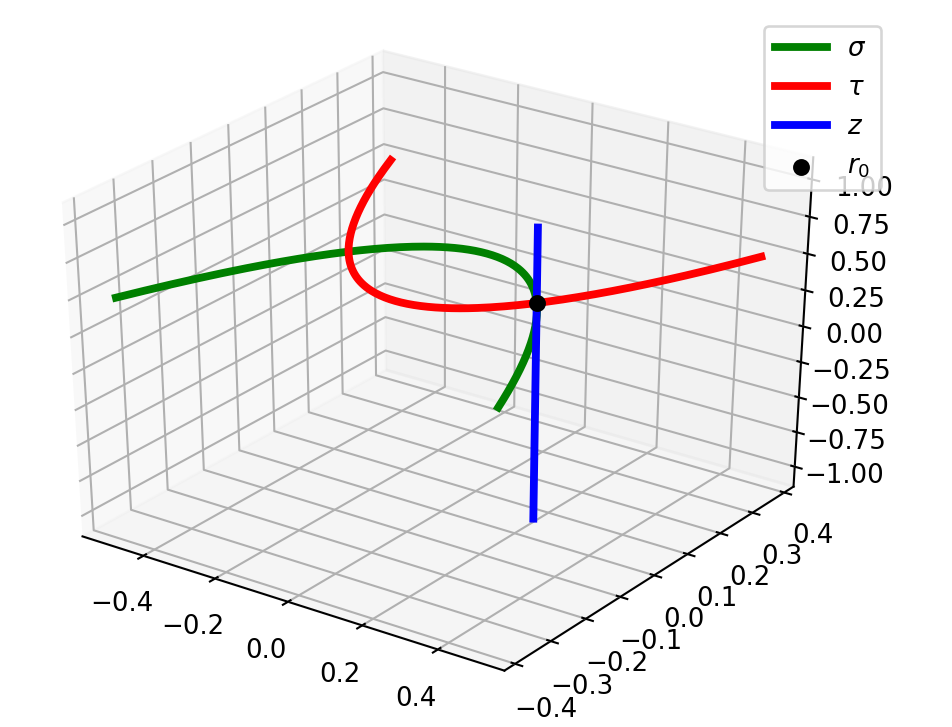
\includegraphics[width=0.4\textwidth]{img/1_2.png}
    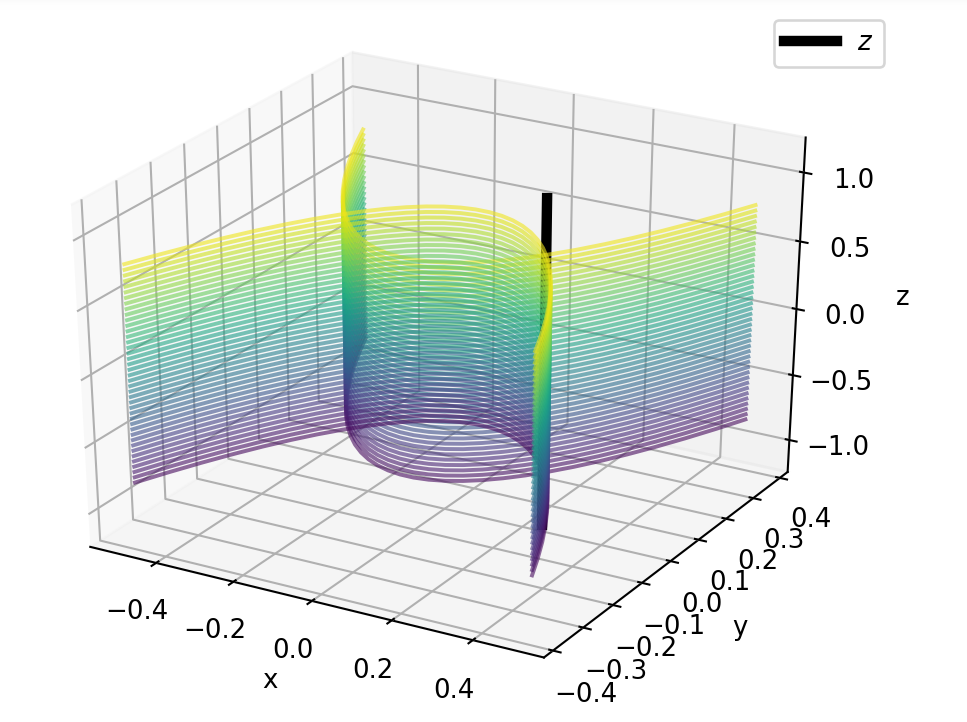
\includegraphics[width=0.4\textwidth]{img/1_2_2.png}
    \caption{Координатные линии и координатные поверхности.}
    \label{fig:1}
\end{figure}

\subsubsection*{Т3.}

Найдём метрический тензор $g_{ij}$ для криволинейных координат 
$(r, \varphi)$, задающих положение точки на параболоиде $z = a(x^2 - y^2)$, при $a=\const$, $x = r \cos \varphi$, $y = r \sin \varphi$.
$$
    \vc{r} = \begin{pmatrix}r \cos{\left(\varphi \right)}\\r \sin{\left(\varphi \right)}\\a r^{2} \cos{\left(2 \varphi \right)}\end{pmatrix};
    \hspace{0.5cm} 
    \vc{g}_i = \frac{\partial \vc{r}}{\partial q^i} 
    \hspace{0.25cm} \Rightarrow \hspace{0.25cm} 
    g_r =\begin{pmatrix}\cos{\left(\varphi \right)}\\\sin{\left(\varphi \right)}\\2 a r \cos{\left(2 \varphi \right)}\end{pmatrix};
    \hspace{0.25cm} 
    g_{\varphi} = \begin{pmatrix}- r \sin{\left(\varphi \right)}\\r \cos{\left(\varphi \right)}\\- 2 a r^{2} \sin{\left(2 \varphi \right)}\end{pmatrix}
$$
Тогда метрический тензор:
\begin{align*}
        g_{ig} &= (\vc{g}_i \cdot \vc{g}_j); \\ 
        g_{11} &= 4 a^{2} r^{2} \cos^{2}{\left(2 \varphi \right)} + \sin^{2}{\left(\varphi \right)} + \cos^{2}{\left(\varphi \right)}; \\
        g_{12} &= g_{21} = - 2 a^{2} r^{3} \sin{\left(4 \varphi \right)}; \\
        g_{22} &= 4 a^{2} r^{4} \sin^{2}{\left(2 \varphi \right)} + r^{2} \sin^{2}{\left(\varphi \right)} + r^{2} \cos^{2}{\left(\varphi \right)}.
\end{align*}
Объединяя, 
$$
    g_{ij} = \begin{pmatrix}16 a^{2} r^{2} \sin^{4}{\left(\varphi \right)} - 16 a^{2} r^{2} \sin^{2}{\left(\varphi \right)} + 4 a^{2} r^{2} + 1 & - 2 a^{2} r^{3} \sin{\left(4 \varphi \right)}\\- 2 a^{2} r^{3} \sin{\left(4 \varphi \right)} & - 16 a^{2} r^{4} \sin^{4}{\left(\varphi \right)} + 16 a^{2} r^{4} \sin^{2}{\left(\varphi \right)} + r^{2}\end{pmatrix}.
$$
Или,
$$
    g^{ij} = (g_{ij})^{-1} = \begin{pmatrix}\frac{- 16 a^{2} r^{2} \sin^{4}{\left(\varphi \right)} + 16 a^{2} r^{2} \sin^{2}{\left(\varphi \right)} + 1}{4 a^{2} r^{2} + 1} & \frac{2 a^{2} r \sin{\left(4 \varphi \right)}}{4 a^{2} r^{2} + 1}\\\frac{2 a^{2} r \sin{\left(4 \varphi \right)}}{4 a^{2} r^{2} + 1} & \frac{16 a^{2} r^{2} \sin^{4}{\left(\varphi \right)} - 16 a^{2} r^{2} \sin^{2}{\left(\varphi \right)} + 4 a^{2} r^{2} + 1}{4 a^{2} r^{4} + r^{2}}\end{pmatrix}.
$$
Соответсвенно,
$$
    \vc{g}^r = g^{rr} g_{r} + g^{r\varphi} g_{\varphi} = 
    \begin{pmatrix}\frac{\left(8 a^{2} r^{2} \sin^{2}{\left(\varphi \right)} + 1\right) \cos{\left(\varphi \right)}}{4 a^{2} r^{2} + 1}\\\frac{\left(8 a^{2} r^{2} \cos^{2}{\left(\varphi \right)} + 1\right) \sin{\left(\varphi \right)}}{4 a^{2} r^{2} + 1}\\\frac{2 a r \cos{\left(2 \varphi \right)}}{4 a^{2} r^{2} + 1}\end{pmatrix};
    \hspace{0.5cm} 
    \vc{g}^{\varphi} = = g^{\varphi r} g_{r} + g^{\varphi \varphi} g_{\varphi} =
    \begin{pmatrix}\frac{\left(- 8 a^{2} r^{2} \sin^{2}{\left(\varphi \right)} + 4 a^{2} r^{2} - 1\right) \sin{\left(\varphi \right)}}{r \left(4 a^{2} r^{2} + 1\right)}\\\frac{\left(8 a^{2} r^{2} \cos^{2}{\left(\varphi \right)} - 4 a^{2} r^{2} + 1\right) \cos{\left(\varphi \right)}}{r \left(4 a^{2} r^{2} + 1\right)}\\- \frac{2 a \sin{\left(2 \varphi \right)}}{4 a^{2} r^{2} + 1}\end{pmatrix}.
$$
На всякий случай проверим в \textit{SymPy}, что
$$
    \vc{g}_r \vc{g}^r = 1; \hspace{0.5cm} 
    \vc{g}_\varphi \vc{g}^{\varphi} = 1; \hspace{0.5cm} 
    \vc{g}_r \vc{g}^{\varphi} = 0; \hspace{0.5cm} 
    g^{ij} g_{ji} = \delta_i^j.
$$
Вот.

\subsubsection*{Т4.} % см. частные производные, когда что-то от чего-то зависит.

Пусть $R = x^2 + y^2 + z^2$, найдём частную производную $\partial R / \partial x$тогда
\begin{enumerate}
    \item $R(x, y, z) = x^2 + y^2 + z^2$. \hfill
        $\partial R / \partial x = 2x$.
    \item $R(x, r, z) = r^2 + z^2$. \hfill
        $\partial R / \partial x = 0$. 
    \item $R(x, y) = x^2 + y^2 + (x^2 - y^2)^2$. \hfill
        $\partial R / \partial x = 2x + 4x(x^2-y^2)$.
    \item $R(x, r) = r^2 + (x^2 - y^2)^2 = r^2 + (2x^2 - r^2)^2$. \hfill
        $\partial R / \partial x = 16x^3 - 8xr^2$.
    \item $R(x, z) = x^2 + (x^2-z) + z^2 = 2x^2 - z + z^2$.\hfill
        $\partial R / \partial x = 4x$.
\end{enumerate}


\subsubsection*{Т5.}
Для первого выражения:
\begin{equation}
    \left.\begin{aligned}
        \frac{\partial \vc{g}^j}{\partial q^k} = \frac{\partial g^{ig}}{\partial q^k} \vc{g}_i + \frac{\partial \vc{g}_i}{\partial q^k} g^{ig}; \\ 
        \vc{g}_i \frac{\partial (\vc{g}^j \cdot \vc{g}^i)}{\partial q^k} = 2 \frac{\partial \vc{g}^i}{\partial q^k} \vc{g}^j \vc{g}_i = 
        2 \frac{\partial \vc{g}^i}{\partial q^k}
    \end{aligned}\right\}
    \hspace{0.5cm} \Rightarrow \hspace{0.5cm} 
    2 \left(\vc{g}_i \cdot \frac{\partial \vc{g}^i}{\partial q^k} \right) + \Gamma_{ijk} = \left(\vc{g}_i  \cdot \frac{\partial \vc{g}^i}{\partial q^k} \right)
    \hspace{0.5cm} \Rightarrow \hspace{0.5cm} 
    (1) = - \Gamma_{ijk} g^{ij}.
\end{equation}

Для второго выражения рассмотрим значение квадрата произведения при фиксированных $i \neq j \neq k$:
$$
    \underbrace{(\vc{g}_i, \vc{g}_j, \vc{g}_k)^2}_{\det g_{mn}} \cdot 
    \underbrace{(\vc{g}^i, \vc{g}^j, \vc{g}^k)^2}_{\det g^{nk}} = \det g_{mn} g^{np} = \det \delta_m^p = 1.
    \hspace{0.5cm} \Rightarrow \hspace{0.5cm} 
    (\vc{g}_i, \vc{g}_j, \vc{g}_k) \cdot (\vc{g}^i, \vc{g}^j, \vc{g}^k) = 3! = 6.
$$
Важно заметить, что $-1$ не является возможным значением произведения таких смешанных произведений, т.к. левой тройке в первом сомножители будет соответствовать тройка во втором сомножителе.

\subsection{Кинематика точки}

\subsubsection*{1.12*}
Параметризуем движение точки некоторым $\varphi(t)$:
\begin{equation}
\label{strsin}
    \left\{\begin{aligned}
        x =  a \cos \varphi\\ 
        y =  b \sin \varphi
    \end{aligned}\right. 
    \hspace{0.25cm} \Rightarrow \hspace{0.25cm} 
    \left\{\begin{aligned}
        \dot{x} &= - a \dot{\varphi} \sin \varphi \\
        \dot{y} &= b \dot{\varphi} \cos \varphi
    \end{aligned}\right.
    \hspace{0.25cm} \Rightarrow \hspace{0.25cm} 
    \left\{\begin{aligned}
        \ddot{x} &= -a \dot{\varphi}^2 \cos \varphi - a \ddot{\varphi} \sin \varphi = 0 \\
        \ddot{y} &= -b \dot{\varphi}^2 \sin \varphi + b \ddot{\varphi} \cos \varphi 
    \end{aligned}\right.
    \hspace{0.25cm} \Rightarrow \hspace{0.25cm} 
    \dot{\varphi}^2 + \ddot{\varphi} \tg \varphi = 0.
\end{equation}
Решением этого уравнения является
$$
    \varphi(t) = \arccos (c_1 + c_2 t).
$$
С учётом начальных условий получим ($x(0)=0$, $\dot{x} = $), что
$$
    \dot{\varphi} 
    c_1 = 0,\hspace{0.5cm} c_2 = \frac{v_0}{a},
    \hspace{0.5cm} \Rightarrow \hspace{0.5cm} 
    \varphi(t) = \arccos (v_0 t / a).
$$
Немного упростим выражения для $\dot{\varphi}$ и $\ddot{\varphi}$:
$$
    \dot{\varphi} = -\frac{v_0}{a \sin \varphi}, \hspace{0.25cm} 
    \ddot{\varphi} = - \frac{\dot{\varphi}^2}{\tg \varphi},
$$
теперь найдём $\ddot{y} (\sin \varphi)$:
$$
    \ddot{y} = - b \dot{f} \sin \varphi + v \ddot{\varphi} \cos \varphi =
    -b \frac{v_0^2}{a^2 \sin^2 \varphi} \sin \varphi - b \left(\frac{v_0}{a} \right)^2 \frac{\cos \varphi}{\sin^2 \varphi \tg \varphi} = 
    - \frac{b}{a^2} v_0^2 \left(\frac{1}{\sin \varphi} + \frac{\cos^2 \varphi}{\sin^3 \varphi} \right) = -\frac{b}{a^2} v_0^2 \frac{1}{\sin^3 \varphi}.
$$ 
Подставив $y = b \sin \varphi$, найдём
$$
    \ddot{y}\left(y = \frac{b}{2} \right) = -\frac{8b}{a^2} v_0^2. 
$$

\subsubsection*{1.19}

Знаем, что в полярных координатах
\begin{equation}
\label{1_2}
    \left\{\begin{aligned}
        r &= \frac{p}{1 + e \cos \varphi}  \\
        r^2 \dot{\varphi} &= c = \const
    \end{aligned}\right.
    \hspace{0.5cm} 
    \text{в полярных координатах}
    \hspace{0.5cm} 
    \left\{\begin{aligned}
        x &= r \cos \varphi \\
        y &= r \sin \varphi
    \end{aligned}\right.
    .    
\end{equation}
Вспомним, что
\begin{align*}
    w_r = \ddot{r} - r \dot{\varphi}^2, \hspace{0.5cm} 
    w_\varphi = \frac{d}{dt} \left(r^2 \dot{\varphi}\right).
\end{align*}
Найдём $\ddot{r}$:
$$
    r + er \cos \varphi = p
    \hspace{0.25cm} \overset{d / d t}{\Rightarrow} \hspace{0.25cm} 
    \dot{r} + e \dot{r} \cos \varphi - e r \dot{\varphi} \sin \varphi = 0
    \hspace{0.25cm} \overset{d / d t}{\Rightarrow} \hspace{0.25cm} 
    \ddot{r} (1 + e \cos \varphi) - e \dot{r} \sin \varphi \left(\dot{\varphi} - \frac{c}{r^2} \right) -\frac{ec}{r} \frac{c}{r^2} \cos \varphi = 0
$$
Выразим и подставим $\dot{\varphi}$ и получим
$$
    \dot{\varphi} = \frac{c}{r^2},
    \hspace{0.5cm} \Rightarrow \hspace{0.5cm} 
    \ddot{r} = \frac{c^2}{r^2 p} \left(\frac{p}{r} -1\right),
    \hspace{0.5cm} \Rightarrow \hspace{0.5cm} 
    \boxed{
    w_r = -\frac{c^2}{pr^2} , \hspace{0.5cm} 
    w_\varphi = 0.}
$$

\subsubsection*{1.37(в)}

Найдём скорость точки и проекции её ускорения на касательные к координатным линиям для координат параболического цилиндра $\sigma, \tau, z$. Для начала найдём координатные векторы и метрический тензор:
$$
    \vc{r} = \begin{pmatrix}
        x \\ y \\ z
    \end{pmatrix} = \begin{pmatrix}
        \sigma \tau \\ \frac{1}{2} (\tau^2 - \sigma^2) \\ z
    \end{pmatrix}
    \hspace{0.5cm} \Rightarrow \hspace{0.5cm} 
        \vc{g}_\sigma = \begin{pmatrix}
        \tau \\ - \sigma \\ 0 
    \end{pmatrix},
    \vc{g}_\tau = \begin{pmatrix}
        \sigma \\ \tau \\ 0
    \end{pmatrix},
    \vc{g}_z = \begin{pmatrix}
        0 \\ 0 \\ 1
    \end{pmatrix}, \hspace{0.5cm} 
    g_{ij} = \begin{pmatrix}
        \tau^2 + \sigma^2 & 0 & \\
        0 & \tau^2 + \sigma^2 & 0 \\
        0 & 0 & 1
    \end{pmatrix}.
$$
Тогда
$$
    v^2 = \dot{\sigma}^2 (\tau^2 + \sigma^2) + \dot{\tau}^2 (\tau^2 + \sigma^2) + \dot{z}^2,
    \hspace{0.5cm} 
    v =  \sqrt{(\dot{\tau}^2 + \dot{\sigma}^2)(\tau^2 + \sigma^2) + \dot{z}^2}
$$
Для $i$-ой ковариантной координаты ускорения верно, что
\begin{equation}
    w_i = \frac{d}{dt} \frac{\partial (v^2/2)}{\partial \dot{q}^i} - \frac{\partial (v^2/2)}{\partial q^i}.
\end{equation}
С учётом коэффициенты Ламе ($H_\tau = H_\sigma=\sqrt{\sigma^2+\tau^2}, H_z = 1$), найдём проекции
\begin{align*}
    w_\tau &= \frac{1}{\sqrt{\sigma^2+\tau^2}} \left(
        \ddot{\tau} (\tau^2 + \sigma^2) + \dot{\tau}^2 \tau  + 2 \dot{\sigma} \dot{\tau} \sigma - \tau \dot{\sigma}^2
    \right); \\
    w_\sigma &= \frac{1}{\sqrt{\sigma^2+\tau^2}} \left(
        \ddot{\sigma} (\tau^2 + \sigma^2) + \dot{\sigma}^2 \sigma  + 2 \dot{\tau} \dot{\sigma} \tau - \sigma \dot{\tau}^2\right); \\
    w_z &= \ddot{z}.
\end{align*}


\subsubsection*{1.45}
Выразим орты сопровождающий трехгранника $(\vc{\tau}, \vc{n}, \vc{b})$ через $\vc{v}$ и $\vc{w}$, с учётом $w \times \vc{v} \neq 0$, $\vc{t} \cdot \vc{v} > 0$.
Так как $\vc{v} \nparallel \vc{w}$, то
$$
    \vc{b} = \frac{\vc{v} \times \vc{w}}{|\vc{v} \times \vc{w}|}.
$$
Выразим $\vc{\tau}$.
$$
    \vc{\tau} = \frac{d \vc{r}}{d s}, \hspace{0.5cm} 
    \vc{v} = \frac{d \vc{r}}{d t} = \frac{ds}{dt} \frac{d \vc{r}}{ds} = v \dot{\tau},
    \hspace{0.5cm} \Rightarrow \hspace{0.5cm} 
    \vc{\tau} = \frac{\vc{v}}{v}.
$$
И найдём $\vc{n} = [\vc{b} \times \vc{\tau}]$, раскрывая двойное векторное произведение (формула Лагранжа), получим
$$
    \vc{n} = \left[\frac{\vc{v}}{v} \times \frac{\vc{v} \times \vc{w}}{|\vc{v} \times \vc{w}|}\right]=
    \frac{\left(\vc{w} \cdot \vc{v}\right)\vc{v} - v^2 \vc{w}}{v |\vc{v} \times \vc{w}|} .
$$

\subsubsection*{Т6.}

Рассмотрим движение точки в цилиндрических координатах:
$$
    \vc{r} = \begin{pmatrix}
        x \\ y \\ z  
    \end{pmatrix} = \begin{pmatrix}
        r \cos \varphi \\ r \sin \varphi \\ z
    \end{pmatrix}
    \hspace{0.5cm} \Rightarrow \hspace{0.5cm} 
    \vc{J} = \begin{pmatrix}
        \cos \varphi & - r \sin \varphi & 0 \\
        \sin \varphi & r \cos \varphi & 0 \\
        0 & 0 & 1
    \end{pmatrix}, \hspace{0.5cm} 
    g_{ij} = \diag(1, r^2, 1)
$$

\begin{wrapfigure}{r}{0.4\textwidth}
  \begin{center}
        \vspace{-5 mm}
        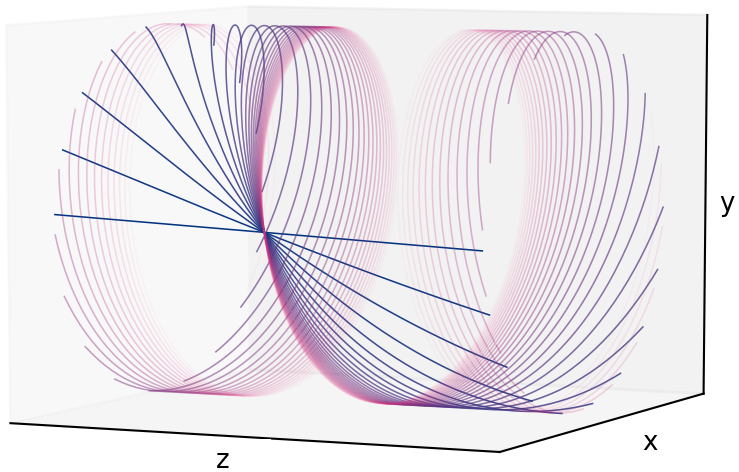
\includegraphics[width=0.9\linewidth]{img/T6_v2.png}
  \end{center}
    \caption{Возможные геодезические цилиндра.}
    \label{fig:cilindre}
\end{wrapfigure}

Для начала выразим ковариантные координаты ускорений:
$$
    w_i = \frac{d}{dt} \frac{\partial (v^2/2)}{\partial q\delta^i} - \frac{\partial (v^2/2)}{\partial q^i} 
    \hspace{0.5cm} \Rightarrow \hspace{0.5cm} 
    \left[\begin{aligned}
        w_r &= \ddot{r} - r \dot{f}^2 \\
        w_\varphi &= \frac{d}{dt} (r^2 \dot{\varphi}) \\
        w_z &= \ddot{z}.
    \end{aligned}\right.
$$
По условию хотим, чтобы $w_\varphi = w_z = 0, r=\const$. Проинтегрировав дважды по времени получим систему уравнений
$$
    \left\{\begin{aligned}
        \varphi &=  c_1 t + c_2;\\
        z &= c_3 t + c_4,
    \end{aligned}\right.
$$
Где $c_1, c_2, c_3, c_4$ --некоторые константы. Построим полученные траектории положив $c_2 = c_4 = 0$ и отмасштабировав к $c_1 = 1$ (см. рис. \eqref{fig:cilindre}).

% \newpage

\subsubsection*{Т7.}
Найдём $\partial v_k / \partial v_j$, при $v_k = v_k(q^i, v^i)$. Далее будем пользоваться тем, что $g_{ig} = g_{ig}(q^i)$.
$$
    v_k(q^i, v^i) = g_{ki} v^i 
    \hspace{0.5cm} \Rightarrow \hspace{0.5cm} 
    \frac{\partial v_k}{\partial v^j} = g_{ki} \frac{\partial v^i}{\partial v^j} = g_{ki} \delta^i_j = g_{kj}.
$$
Теперь найдём $\partial v_k / \partial q^j$, при $v_k = v_k(q^i, v^i)$. 
$$
    \frac{\partial v_k(q^i, v^i)}{\partial q^j} = v^i \left(
        \frac{\partial  g_{ki}}{\partial q^j} 
    \right) = v^i \left(
        \left(\frac{\partial \vc{g}_k}{\partial q^j}, \, \vc{g}_i \right) +
        \left(\frac{\partial \vc{g}_i}{\partial q^j}, \, \vc{g}_k\right)
    \right) = v^i\left(\Gamma_{ijk} + \Gamma_{kji}\right).
$$
Теперь найдём $\partial v_k / \partial q^j$, при $v_k = v_k(q^i, v_i)$. Но тут так как функция выражается через саму себя, то при частном дифференцировании, $v_k = \const$, тогда $\partial v_k(q^i, v_i) / \partial q^j = 0$.



\subsubsection*{Т8.*}
Найдём $v_i \dot{v}^i - v^i \dot{v}_i$. Перейдём к контравариантным координатам:
$$
    v_i \dot{v}^i - v^i \dot{v}_i = g_{ij} v^i v^j - v^i \frac{d}{dt} \left(
             g_{ij} v^j
        \right) =    g_{ij} v^j \dot{v}^i  - v^i v^j \dot{g}_{ij} - g_{ij} v^i \dot{v}^j
$$
В силу симметричности метрического тензора $g_{ij}=g_{ji}$, получим, что
$$
    v_i \dot{v}^i - v^i \dot{v}_i =  - v^i v^j \dot{g}_{ij}.
$$
Подставил для параболических и полярных координат, сходится.

\subsection{Кинематика твёрдого тела}

\subsubsection*{3.24}


\begin{wrapfigure}{r}{0.35\textwidth}
  \begin{center}
        \vspace{-10 mm}
        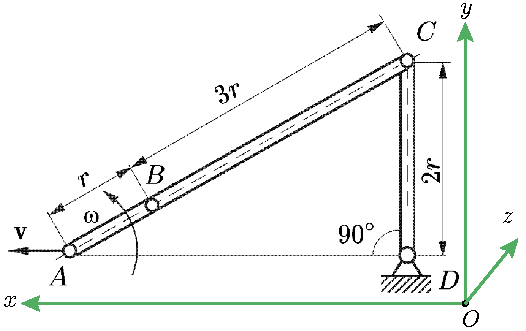
\includegraphics[width=0.9\linewidth]{img/3_24.pdf}
  \end{center}
    \caption{К задаче 3.24.}
    %\label{fig:}
\end{wrapfigure}


Запишем $\vc{v}_B$, выбрав в качестве полюса точку $A$ и точку $C$.
\begin{align}
\label{vb}
    \vc{v}_{B} = \vc{\omega} \times \vv{AB} + \vc{v} = \vc{v}_{C} + \vc{\omega}_{BC} \times \vv{CB},
\end{align}
или, расписав по координатам,
$$
\underbrace{\begin{pmatrix}
        0 \\ 0 \\ \omega
    \end{pmatrix} \times \begin{pmatrix}
        - r \cos \alpha \\
        r \sin \alpha \\
        0
    \end{pmatrix}}_{\vc{\omega} \times \vv{AB}}
    + \begin{pmatrix}
        v \\
        0 \\
        0
    \end{pmatrix} =
    \begin{pmatrix}
        v_C \\
        0 \\
        0
    \end{pmatrix} +
    \begin{pmatrix}
        0 \\
        0 \\
        \omega_{BC}
    \end{pmatrix} \times
    \begin{pmatrix}
        3r \cos \alpha \\
        3r \sin \alpha \\
        0
    \end{pmatrix},
$$
получим два содержательных уравнения
$$
    \left.\begin{aligned}
        -r\omega \sin \alpha + v &= v_c + 3r \omega_{BC} \sin \alpha \\
        -r\omega \cos \alpha  + 0&= 0 \;\, + 3r \omega_{BC} \cos \alpha
    \end{aligned}\right\}
    \hspace{0.5cm} \Rightarrow \hspace{0.5cm} 
    \boxed{
    \vc{\omega}_{BC} = -\frac{\vc{\omega}}{3},
    \hspace{0.5cm} \vc{v}_C = \vc{v}.
    }
$$

\phantom{42}    

Для поиска $\vc{\mathrm{w}}_C$, запишем условия жёсткости стержней $BC$ и $CD$. Дифференцируя по времени, получим
\begin{equation}
\label{eq_12}
        \left.\begin{aligned}
            \vc{v}_B \cdot \vv{BC} &= \vc{v}_C \cdot \vv{BC}; \\
             \vc{v}_C \cdot \vv{DC} &= 0.
        \end{aligned}\right\}
    \hspace{0.25cm} \overset{d / dt}{\Rightarrow}  \hspace{0.25cm} 
        \left\{\begin{aligned}
        \vc{\mathrm{w}}_B \cdot \vv{BC} + \vc{v}_B \cdot \dot{\vv{BC}} &=
        \vc{\mathrm{w}}_C \cdot \vv{BC} + \vc{v}_C \cdot \dot{\vv{BC}}; \\
        \vc{\mathrm{w}}_C \cdot \vv{DC} + \vc{v}_C \cdot \dot{\vv{DC}} &= 0.
        \end{aligned}\right.
\end{equation}
Выразим $\vc{\mathrm{w}}_B$ из уравнения Ривальса:
$$
    \vc{\mathrm{w}}_B = \underbrace{\vc{\mathrm{w}}_A}_{0} + \underbrace{\dot{\omega}_{AB} \times \vv{AB}}_{0} +
    \,
     \vc{\omega} \times \left(
        \vc{\omega} \times \vv{AB}
    \right) = \begin{pmatrix}
        0 \\ 0 \\ \omega
    \end{pmatrix} 
    \begin{pmatrix}
        -r\omega\sin\alpha \\
        -r\omega\cos\alpha \\
        0
    \end{pmatrix} = \begin{pmatrix}
        r\omega^2 \cos \alpha \\
        -r\omega^2 \sin \alpha \\
        0
    \end{pmatrix}.
$$
В первом уравнении \eqref{eq_12}, зная $\dot{\vv{BC}} = \vc{\omega}_{BC} \times \vv{BC} = (\omega r \sin \alpha,\; \omega r \cos \alpha,\; 0)\T$ и $\vc{v}_B$ из \eqref{vb}, получим
\begin{equation}
    \label{eqI}
    \vc{\mathrm{w}}_C \cdot \vv{BC} = - 4 \omega^2 r^2.
\end{equation}
Во втором уравнении \eqref{eq_12}, зная $\dot{\vv{DC}} = \vc{\omega}_{DC} \times \vv{DC} = \vc{v}_C$, получим
\begin{equation}
    \label{eq2}
    \vc{\mathrm{w}}_C \cdot \vv{DC} = -v^2.
\end{equation}
Из \eqref{eq2}, мы знаем $(\vc{\mathrm{w}}_C)_y$, расписав в \eqref{eqI} проекцию на $BC$ покоординатно, получим
$$
    \left.\begin{aligned}
        -4 \omega^2 r^2 &= 3r (-{\mathrm{w}}_{Cx} \cos \alpha + {\mathrm{w}}_{Cy} \sin \alpha); \\
        {\mathrm{w}}_{Cy} &= -{v^2}/{2r} .
    \end{aligned}\right\}
    \hspace{0.5cm} \Rightarrow \hspace{0.5cm} 
        \vc{\mathrm{w}}_C = 
        \begin{pmatrix}
            \mathrm{w}_{Cx} \\
            \mathrm{w}_{Cy} \\
            0
        \end{pmatrix},
    \hspace{0.25cm} \text{где} \hspace{0.25cm} 
    \mathrm{w}_{Cx} = \frac{8\sqrt{3}}{9} \omega^2 r - \frac{\sqrt{3}}{6} \frac{v^2}{r}, \;
    \mathrm{w}_{Cy} = -\frac{v^2}{2r}.
$$
Собственно\footnote{
    Вычисления доступны здесь.
}, $\|\vc{\mathrm{w}}_C\|^2 = \frac{64}{27}\omega^{4} r^{2} - \frac{8 }{9}\omega^{2} v^{2} + \frac{1}{3} {v^{4}}/{ r^{2}} $.


%%%%%%%%%%%%%%%%%%%%%%%%%%%%%%%%%%%%%%%%%%%%%%%%%%%%%%%%%%%%%%%%%%%%%%%%%%%%%%%%%%%


\subsubsection*{4.4}



Запишем в координатах $\omega_1$ и $\omega_2$.
$$
    \vc{\omega}_1 = \begin{pmatrix}
        0 \\ \omega_1 \sin \theta \\ \omega_1 \cos \theta
    \end{pmatrix};
    \hspace{0.5cm} 
    \vc{\omega}_2 = \begin{pmatrix}
        0 \\ 0 \\ \omega_2
    \end{pmatrix}.
$$

Так как оси $\omega_1$  и $\omega_2$ пересекаются, угловая скорость и угловое ускорение можно найти, как
$$
    \vc{\omega} = \vc{\omega}_1 + \vc{\omega}_2 = \begin{pmatrix}
        0 \\ \omega_1 \sin \theta \\ \omega_2 + \omega_1 \cos \theta
    \end{pmatrix},
    \hspace{1cm} 
    \vc{\varepsilon} = \vc{\omega}_1 \times \vc{\omega}_2 = \begin{pmatrix}
        \omega_1 \omega_2 \sin \theta \\ 0 \\ 0
    \end{pmatrix},
$$
что очень похоже на правду.

\begin{center}
    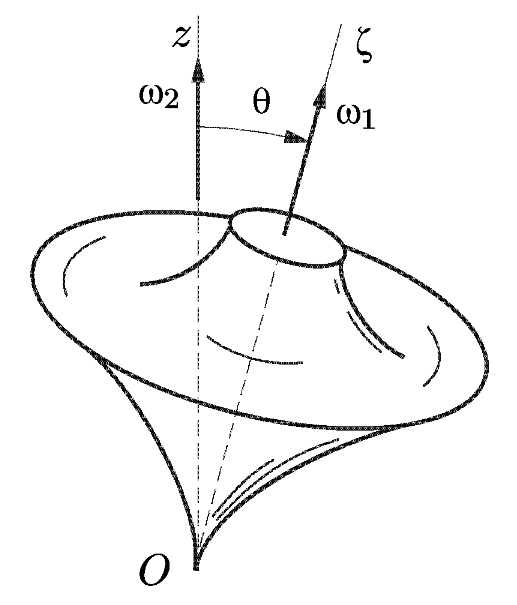
\includegraphics[width=0.2\textwidth]{img/4_4.png}
    \hspace{3cm} 
    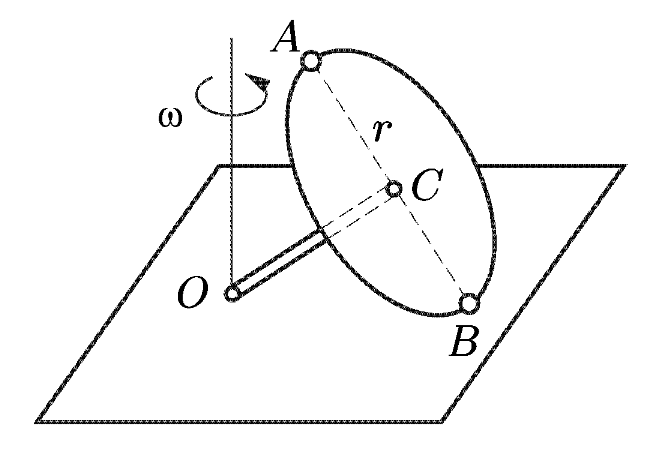
\includegraphics[width=0.3\textwidth]{img/4_10.png}\\
    Рисунки к задачам 4.4 и 4.10.
\end{center}

%%%%%%%%%%%%%%%%%%%%%%%%%%%%%%%%%%%%%%%%%%%%%%%%%%%%%%%%%%%%%%%%%%%%%%%%%%%%%%%%%%%
\subsubsection*{4.10}

Запишем $\vc{v}_c$, как результат движения стержня и диска. Пусть $\Omega$ -- угловая скорость вращения диска, $\parallel OB$.
$$
    \vc{v}_C = \vc{\Omega} \times \vv{BC} = \vc{\Omega} \times \vv{OC} =
    \vc{\omega} \times \vv{OC}.
$$
Другими словами, в координатной записи,
$$
    \begin{pmatrix}
        \Omega \\ 0 \\ 0
    \end{pmatrix} \times \begin{pmatrix}
        3 \\ \sqrt{3} \\ 0
    \end{pmatrix} \frac{r}{2}  = \begin{pmatrix}
        0 \\ \omega \\ 0
    \end{pmatrix} \times \begin{pmatrix}
        3 \\ \sqrt{3} \\ 0
    \end{pmatrix} \frac{r}{2}
    \hspace{0.5cm} \Rightarrow \hspace{0.5cm} 
    \boxed{\Omega = - \sqrt{3} \omega}.
$$
Угловое ускорение стержня найдём, как движение в СО стержня,
$$
    \vc{\varepsilon}^a = \vc{\varepsilon} + \vc{\varepsilon}^r + \vc{\omega} \times \vc{\Omega} =
    \begin{pmatrix}
        0 \\ \varepsilon \\ 0
    \end{pmatrix} +
    \begin{pmatrix}
        -\sqrt{3}\varepsilon \\ - \varepsilon \\ 0
    \end{pmatrix} +
    \begin{pmatrix}
        0 \\0 \\ \sqrt{3} \omega^2
    \end{pmatrix} = \begin{pmatrix}
        - \sqrt{3} \varepsilon \\ 0\\ \sqrt{3} \omega^2
    \end{pmatrix}
    \hspace{0.5cm} \Rightarrow \hspace{0.5cm} 
    \boxed{\varepsilon^a = \sqrt{3\left(\varepsilon^2 + \omega^4\right)}},
$$
где
$$
    \vc{\varepsilon}^r = \vc{\dot{\omega}} = \frac{d}{dt} \left(\vc{\Omega} - \vc{\omega}\right) = \frac{d}{dt} \begin{pmatrix}
        - \sqrt{3} \omega \\ -\omega \\ 0
    \end{pmatrix} = \begin{pmatrix}
        - \sqrt{3} \varepsilon \\ - \varepsilon \\ 0
    \end{pmatrix}.
$$
Теперь, из сложения ускорений,
$$
    \vc{\mathrm{w}}^a = \underbrace{\vc{\mathrm{w}}_0 + \vc{\varepsilon} \times \vc{r} + \vc{\omega} \times \vc{\omega} \times \vc{r}}_{\vc{\mathrm{w}}^e} + \underbrace{2 \vc{\omega} \times \vc{v}^r}_{\vc{\mathrm{w}}^c} + \vc{\mathrm{w}}^r,
$$
найдём $\vc{\mathrm{w}}_B^a$:
$$
    \vc{\mathrm{w}}_B^a = \vc{0} + \vc{\varepsilon} \times \vv{OB} + \vc{\omega} \times \left(
        \vc{\omega} \times \vv{OB}
    \right) + 2 \vc{\omega} \times \left(- \vc{\omega} \times \vv{OB} \right) + \vc{\mathrm{w}}^r_B.
$$
Теперь найдём $\vc{\mathrm{w}}^r_B$, как
$$
    \vc{\mathrm{w}}^r_B = \vc{\mathrm{w}}_{\tau}^r + \vc{\mathrm{w}}_n^r =
    - \varepsilon r \begin{pmatrix}
        \sqrt{3} \\ 1 \\ 0
    \end{pmatrix} \times \begin{pmatrix}
        2 \\ 0 \\ 0
    \end{pmatrix} + \omega^2 \frac{1}{2} \begin{pmatrix}
        - r \\ r \sqrt{3} \\ 0
    \end{pmatrix}.
$$
Подставляя, дойдём до
$$
    \boxed{\vc{\mathrm{w}}_B^a = \begin{pmatrix}
        0 \\ 2 \sqrt{3} \omega^2 r \\ 0
    \end{pmatrix}}
    \hspace{0.5cm} \Rightarrow \hspace{0.5cm} 
    \|\vc{\mathrm{w}}^r_B\| = 2 \sqrt{3} \omega^2 r,
$$
что, достаточно, логично.

Аналогично найдём $\vc{\mathrm{w}}^r_A$:
$$
    \vc{\mathrm{w}}^r_B = \vc{0}  + \begin{pmatrix}
        0 \\ \varepsilon \\ 0 
    \end{pmatrix} \times \begin{pmatrix}
        1 \\ \sqrt{3} \\ 0
    \end{pmatrix} r - \begin{pmatrix}
        0 \\ \omega \\ 0
    \end{pmatrix} \times
    \begin{pmatrix}
        0 \\ \omega \\ 0
    \end{pmatrix} \times
    \begin{pmatrix}
        1 \\ \sqrt{3} \\ 0
    \end{pmatrix} r +
    2 \omega^2 r \begin{pmatrix}
        1 \\ -\sqrt{3} \\ 0
    \end{pmatrix} - \varepsilon r \begin{pmatrix}
        0 \\ 0 \\ 2
    \end{pmatrix},
    \hspace{0.2cm} \Rightarrow \hspace{0.2cm} 
    \boxed{\vc{\mathrm{w}}^r_B = r \begin{pmatrix}
        3 \omega^2 \\ 2 \sqrt{3} \omega^2 \\ - 3 \varepsilon 
    \end{pmatrix}}.
$$
И найдём норму ускорения точки $A$
$$
    \|\vc{\mathrm{w}}_A^a\| = \sqrt{21 \omega^4 r^2 + 9 \varepsilon^2 r^2}.
$$


%%%%%%%%%%%%%%%%%%%%%%%%%%%%%%%%%%%%%%%%%%%%%%%%%%%%%%%%%%%%%%%%%%%%%%%%%%%%%%%%%%%
\subsubsection*{4.12}

\begin{wrapfigure}{r}{0.35\textwidth}
  \begin{center}
        \vspace{-14 mm}
        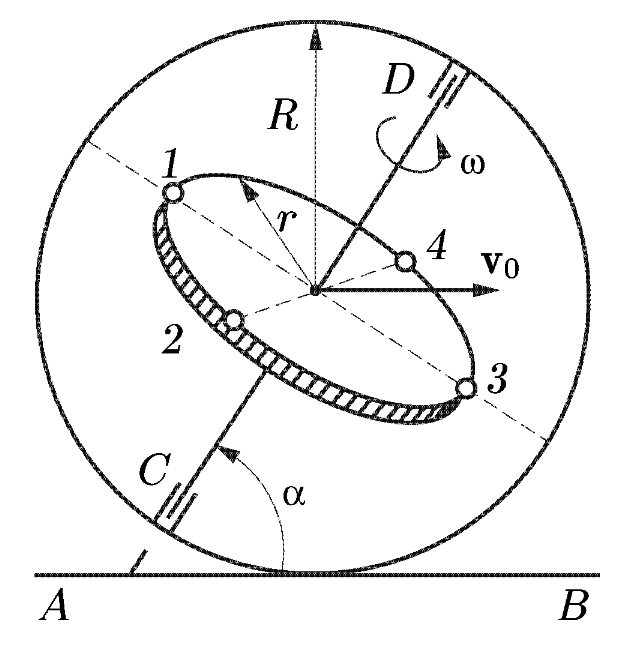
\includegraphics[width=0.8\linewidth]{img/4_12.png}
  \end{center}
    % \caption*{К задаче 4.12}
    %\label{fig:}
\end{wrapfigure}


Расмотрим движение интересных нам точек, как движение в СО обруча, с
$$
    \vc{v}^e = \vc{v} = \begin{pmatrix}
        v \\ 0\\ 0
    \end{pmatrix};
    \hspace{0.5cm} 
    \vc{\omega}^e = \begin{pmatrix}
        0 \\ 0 \\ - v / R
    \end{pmatrix};
    \hspace{0.5cm} \vc{\mathrm{w}}^e = \vc{0};
    \hspace{0.5cm} \vc{\varepsilon}^e = \vc{0}.
$$
Найдём радиус векторы до интересных нам точек:
$$
    \vv{O1} = \begin{pmatrix}
        -r \sin \alpha \\ r \cos \alpha \\ 0
    \end{pmatrix};
    \hspace{0.5cm} 
    \vv{O2} = \begin{pmatrix}
        0 \\ 0 \\ r
    \end{pmatrix};
    \hspace{0.5cm} 
    \vv{O3} = \begin{pmatrix}
        r \sin \alpha \\ -r \cos \alpha \\ 0
    \end{pmatrix};
    \hspace{0.5cm} 
    \vv{O4} = \begin{pmatrix}
        0 \\ 0 \\ -r
    \end{pmatrix}.
$$
Тогда, из теоремы о сложении скоростей, получим значения для $\vc{v}_i^a$:
$$
    \vc{v}_i^a = \underbrace{\vc{v} + \vc{\omega}^e \times \vv{Oi}}_{\vc{v}^e_i} + \underbrace{\vc{\omega}^r \times \vv{Oi}}_{\vc{v}^r_i}.
$$
Подставляя значения, получим, что
\begin{align*}
\vc{v}_1^a = 
\left(\begin{matrix}{v \left(R + r \cos{\alpha}\right)}/{R} \\ {r v \sin{\alpha}}/{R}\\\omega r\end{matrix}\right),
% 
\hspace{0.2cm} 
% 
\vc{v}_2^a = 
\left(\begin{matrix}\omega r \sin{\alpha} + v\\- \omega r \cos{\alpha }\\0\end{matrix}\right),
% 
\hspace{0.2cm} 
\vc{v}_3^a = 
\left(\begin{matrix}{v \left(R - r \cos{\alpha}\right)}/{R}\\- {r v \sin{\alpha}}/{R}\\- \omega r\end{matrix}\right),
% 
\hspace{0.2cm} 
\vc{v}_4^a = 
\left(\begin{matrix}- \omega r \sin{\alpha} + v\\\omega r \cos{\alpha}\\0\end{matrix}\right).
\end{align*}
Или, переходя к значениями $\|\vc{v}_i^a\|$:
\begin{align*}
& \|\vc{v}_1^a\| = \left(/{R^{2} \omega^{2} r^{2} + R^{2} v^{2} + 2 R r v^{2} \cos{\left(\alpha \right)} + r^{2} v^{2}}\right)/{R^{2}}, 
% 
& \|\vc{v}_2^a\| = \omega^{2} r^{2} + 2 \omega r v \sin{\left(\alpha \right)} + v^{2}, \\
% 
& \|\vc{v}_3^a\| = \left({R^{2} \omega^{2} r^{2} + R^{2} v^{2} - 2 R r v^{2} \cos{\left(\alpha \right)} + r^{2} v^{2}}\right)/{R^{2}}, 
% 
& \|\vc{v}_4^a\| = \omega^{2} r^{2} - 2 \omega r v \sin{\left(\alpha \right)} + v^{2}.
\end{align*}
Что соответсвует ответам учебника.

Теперь, из теоремы о сложении скоростей, найдём $\vc{\mathrm{w}}^a_i$
$$
    \vc{\mathrm{w}}^a_i = \underbrace{0 + \vphantom{\left(\vv{Oi}\right)} 0 + \vc{\omega}^e \times \vc{\omega}^e \times \vv{Oi}}_{\vc{\mathrm{w}}^e} + \underbrace{2 \vc{\omega}^e \times \left(
        \vc{\omega}^r \times \vv{Oi}
    \right)}_{\vc{\mathrm{w}}^c} + \underbrace{\vphantom{\left(\vv{Oi}\right)} -\omega^2 \cdot \vv{Oi}}_{\vc{\mathrm{w}}^r_i}.
$$
Подставляя значения, получим, что
\begin{align*}
% 
& \vc{\mathrm{w}}^a_1 = \frac{r \left(R^{2} \omega^{2} + v^{2}\right) }{R^2} 
\left(\begin{matrix}{\sin{\alpha}}\\- { \cos{\alpha}}\\0\end{matrix}\right),
% 
& \vc{\mathrm{w}}^a_2 = - \omega r
\left(\begin{matrix} {2 v \cos{\alpha}}/{R}\\ {2 v \sin{\alpha}}/{R}\\ \omega \end{matrix}\right), \\
% 
& \vc{\mathrm{w}}^a_3 = \frac{r \left(R^{2} \omega^{2} + v^{2}\right) }{R^2} 
\left(\begin{matrix}- { \sin{\alpha}}\\{\cos{\alpha}}\\0\end{matrix}\right),
% 
& \vc{\mathrm{w}}^a_4 = \omega r
\left(\begin{matrix}{2 v \cos{\alpha}}/{R}\\{2 v \sin{\alpha}}/{R}\\\omega \end{matrix}\right).
% 
\end{align*}
Или, переходя к нормам, получим, что
\begin{align*}
    &\|\vc{\mathrm{w}}^a_1\|=\frac{r^{2} \left(R^{2} \omega^{2} + v^{2}\right)^{2}}{R^{4}}
    , 
    &\|\vc{\mathrm{w}}^a_2\|=\frac{\omega^{2} r^{2} \left(R^{2} \omega^{2} + 4 v^{2}\right)}{R^{2}}
    , 
    &\|\vc{\mathrm{w}}^a_3\|=\frac{r^{2} \left(R^{2} \omega^{2} + v^{2}\right)^{2}}{R^{4}}
    , 
    &\|\vc{\mathrm{w}}^a_4\|=\frac{\omega^{2} r^{2} \left(R^{2} \omega^{2} + 4 v^{2}\right)}{R^{2}}.
\end{align*}



%%%%%%%%%%%%%%%%%%%%%%%%%%%%%%%%%%%%%%%%%%%%%%%%%%%%%%%%%%%%%%%%%%%%%%%%%%%%%%%%%%%
\subsubsection*{4.32}


Нам известно $\vc{r}(t) = (x(t), y(t), z(t))\T$, из задачи \textbf{1.45} знаем, как выразить
направляющие трёхгранника Френе $\vc{\tau}, \vc{\nu}, \vc{\beta}$, через $\vc{\dot{r}}$ и $\vc{\ddot{r}}$, соотвественно считаем известными $\rho, \varkappa$. В выводе теоремы сложения ускорений использовалось, что
\begin{equation}
\label{432_1}
    \frac{d \vc{e}_i}{dt} = \vc{\omega}^e \times \vc{e}_i.
\end{equation}
Также мы знаем, что
\begin{equation}
\label{432_2}
    \frac{d \vc{\tau}}{ds} = \frac{1}{\rho} \vc{\nu},
    \hspace{0.5cm}
    \frac{d \vc{\nu}}{ds} = -\frac{1}{\rho}  \vc{\tau} + \varkappa \vc{\beta},
    \hspace{0.5cm} 
    \frac{d \vc{\beta}}{d s} = - \varkappa \vc{\nu}.
\end{equation}
Тогда, из покоординатной записи, в $(\vc{\tau}, \vc{\nu}, \vc{\beta})$,получим систему уравнений, решая которую получим
$$
    \left.\begin{aligned}
        \frac{d \vc{\tau}}{dt}  &= \frac{d \vc{\tau}}{ds} v \\
        \frac{d \vc{\beta}}{d t} &= \frac{d \vc{\beta}}{d s} v 
    \end{aligned}\right\}
    \hspace{0.5cm} \Rightarrow \hspace{0.5cm} 
    \left.\begin{aligned}
        \frac{1}{\rho} \vc{\nu} v &= \vc{\omega} \times \vc{\tau} \\
        - v \varkappa \vc{\nu} &= \vc{\omega} \times \vc{\beta}
    \end{aligned}\right\}
    \hspace{0.5cm} \Rightarrow \hspace{0.5cm} 
    \left.\begin{aligned}
        \omega_1 &= v \varkappa \\
        \omega_2 &= 0 \\
        \omega_3 &= v / \rho
    \end{aligned}\right\}
    \hspace{0.5cm} \Rightarrow \hspace{0.5cm} 
    \boxed{
         \omega = (\vc{v} \cdot \vc{\tau}) (\varkappa \vc{\tau} + \vc{\beta} / \rho)   
    }.
$$

%%%%%%%%%%%%%%%%%%%%%%%%%%%%%%%%%%%%%%%%%%%%%%%%%%%%%%%%%%%%%%%%%%%%%%%%%%%%%%%%%%%
\subsubsection*{4.37}

Пусть $\vc{\omega}^r$ -- угловая скорость тела в СО Земли, посмотрим на угловое ускорение твёрдого тела относительно СО, в данный момент времени совпадащей с направлениями: $\vc{e}_i \parallel \vc{\omega}_i$, с полюсом в неподвижной точке тела.
$$
    \vc{\varepsilon}^a = \frac{d \omega}{d t} = 
    \dot{\omega}_1 \frac{\vc{\omega}_1}{\omega_1} +
    \dot{\omega}_2 \frac{\vc{\omega}_2}{\omega_2} +
    \dot{\omega}_3 \frac{\vc{\omega}_3}{\omega_3} + \vc{\omega} \times \vc{\omega} = 
    \dot{\omega}_1 \frac{\vc{\omega}_1}{\omega_1} +
    \dot{\omega}_2 \frac{\vc{\omega}_2}{\omega_2} +
    \dot{\omega}_3 \frac{\vc{\omega}_3}{\omega_3},
$$
так как оси жёстко связаны с самим телом.


%%%%%%%%%%%%%%%%%%%%%%%%%%%%%%%%%%%%%%%%%%%%%%%%%%%%%%%%%%%%%%%%%%%%%%%%%%%%%%%%%%%
\subsubsection*{4.50}

Знаем, что скорость некоторой точки твёрдого тела можем записать, как
$$
    \vc{v} = \vc{v}_0 + \vc{\omega}\times \vc{r} = \vc{v}_0 + \begin{pmatrix}
        \omega_y r_z - \omega_z r_y \\
        \omega_z r_x - \omega_x r_z \\
        \omega_x r_y - \omega_y r_x
    \end{pmatrix}.
$$
Тогда, прямой подстановкой, получим, что
$$
    \rot \vc{v} = \cancel{\rot \vc{v}_0} +
    \rot \begin{pmatrix}
        \omega_y r_z - \omega_z r_y \\
        \omega_z r_x - \omega_x r_z \\
        \omega_x r_y - \omega_y r_x
    \end{pmatrix} =
    2 \begin{pmatrix}
        \omega_x \\ \omega_y \\ \omega_z
    \end{pmatrix},
    \hspace{0.5cm} \Rightarrow \hspace{0.5cm} 
    \vc{\omega} = \frac{1}{2} \rot \vc{v} .
$$

\subsection{Сложное движение точки и твёрдого тела}

\subsubsection*{4.14 и 4.15*}

Сделаем задачу чуть менее абстрактной. Представим кольцевую железную дорогу, плоскость которой нормальна к $\vc{\omega}_1$. Наш агент  \textnumero 1 сидит в вагоне поезда и на столе, поверхность которого нормальна к $\vc{\omega}_2$, запускает игрушечную кольцевую жилезную дорогу с игрушечным агентом  \textnumero 2 в вагоне поезда. Агент  \textnumero 2 запускает поезд на столе, поверхность которого нормальна к $\vc{\omega}_3$ ...

Найдём $\vc{\varepsilon}_{\text{\textnumero} 2}$ -- угловое ускорение агента \textnumero 2. По словам \textnumero 1, угловое ускорение равно $\vc{\omega}_{\text{\textnumero 2}} = \vc{\omega}_2$, тогда
$$
    \vc{\varepsilon}_{\text{\textnumero} 2} = \underbrace{\vc{\varepsilon}_1}_{\vc{\varepsilon}^e} + \frac{d}{dt} \vc{\omega}_2 = 0 + 
    \frac{\vc{\omega}_2}{\omega_2} \dot{\omega}_2
    + 
    \vc{\omega}_1 \times \vc{\omega}_2.
$$
А теперь найдём $\vc{\varepsilon}_3$. С точки зрения \textnumero 2 $\vc{\omega}_{\text{\textnumero 3}} = \vc{\omega}_3$. Мы знаем, что $\vc{\omega}_{\text{\textnumero 2}} = \vc{\omega}_1 + \vc{\omega}_2$, и знаем $\vc{\varepsilon}_{\text{\textnumero} 2}$, тогда
$$
    \vc{\varepsilon}_{\text{\textnumero} 3} = \vc{\varepsilon}_2 + \frac{d}{dt} \vc{\omega}_3 = 
    \left(\frac{\vc{\omega}_2}{\omega_2} \dot{\omega}_2 + \vc{\omega}_1 \times \vc{\omega}_2\right)
    + 
    \frac{\vc{\omega}_3}{\omega_3} \dot{\omega}_3
    + 
    (\vc{\omega}_1 + \vc{\omega}_2) \times \vc{\omega}_3.
$$
И так далее мы можем продолжать добавлять вектора $\vc{\omega}_i$ к движению тела, в силу $\vc{\omega}^a = \vc{\omega}^e + \vc{\omega}^r$, при чём мы получим слагаемые вида векторного произведение всех упорядоченных пар $\vc{\omega}_j$ и $\vc{\omega}_k$, плюс сумма $\vc{\varepsilon}^r_i$.
$$
    \vc{\varepsilon}_{\text{\textnumero} N} = \vc{\varepsilon}_{\text{\textnumero} (N-1)} + 
    \frac{\vc{\omega}_N}{\omega_N} \dot{\omega}_N +
    \vc{\omega}_{\text{\textnumero} (N-1)} \times \vc{\omega}_N.
$$
По индукции можем показать, что
$$
    \vc{\varepsilon} = \vc{\varepsilon}_{\text{\textnumero} N} = \sum_{j=2}^n \frac{\vc{\omega}_j}{\omega_j} \dot{\omega}_j + \sum_{k=2}^N \sum_{i=1}^{k-1} \vc{\omega}_i \times \vc{\omega}_k.
$$
В частности, при $\dot{\omega}_j = 0$, получим выражение для задачи \textbf{4.14}.


%%%%%%%%%%%%%%%%%%%%%%%%%%%%%%%%%%%%%%%%%%%%%%%%%%%%%%%%%%%%%%%%%%%%%%%%%%%%%%%%%%%
\subsubsection*{Т9.*}


\begin{wrapfigure}{r}{0.24\textwidth}
  \begin{center}
        % \vspace{-15 mm}
        \incfig{1}    
  \end{center}
    %\caption{}
    %\label{fig:}
\end{wrapfigure}

Рассмотрим движение выпуклого твёрдого тела по выпуклой поверхности. В конкретный момент времени они соприкасаются в точках $A$ и $C$ соответсвенно. Можно рассматривать это как движение шара с радиусом кривизын равным радиусу кривизны $r$ твёрдого тела в точке $A$, по плоскости, содержащей точку $C$. 

Тогда, по формуле Ривальса,
$$
    \vc{\mathrm{w}}_A = \vc{\mathrm{w}}_O + \vc{\varepsilon} \times \vc{r} + \omega \times (\vc{\omega} \times \vc{r}).
$$
А скорость точки $C$, относительно твёрдого тела, совпадает с точностью до знака, со скоростью точки $O$, относительно поверхности, то есть 
$$
    \vc{v}= \vc{v}_O = \vc{v}_C = \vc{\omega} \times (-\vc{r}),
$$
где $\vc{r} = \vv{OA}$. 

Теперь заметим, что
$$
    d \vc{v} = d \vc{\omega} \times (-\vc{r}) + \vc{\omega} \times (- \d \vc{r})
     = (\vc{\varepsilon} \d t) \times (-\vc{r}),
     \hspace{0.5cm} \Rightarrow \hspace{0.5cm} 
     \vc{\mathrm{w}}_A = \frac{d \vc{v}}{d t}  = \vc{\varepsilon} \times (-\vc{r})
$$
И, собирая всё вместе, получим, что
$$
    \vc{\mathrm{w}}_A = \vc{\varepsilon} \times (-\vc{r}) + \vc{\varepsilon} \times \vc{r} + \omega \times (-\vc{v}) = - \vc{\omega} \times \vc{v},
$$
что и требовалось доказать.




\subsection{Сложное движение точки и твёрдого тела}

\subsubsection*{2.15}

% \begin{wrapfigure}{r}{0.25\textwidth}
%   \begin{center}
%         \vspace{-20 mm}
%         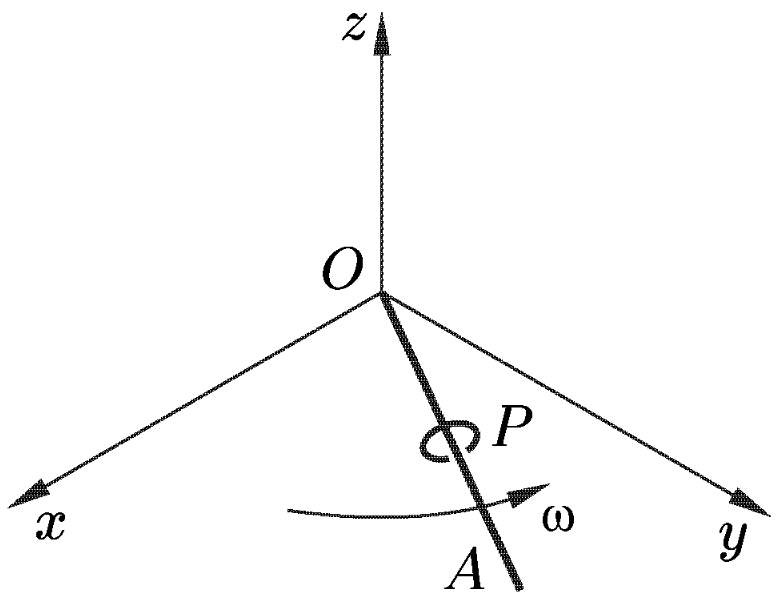
\includegraphics[width=0.8\linewidth]{img/2_15.png}
%   \end{center}
% \end{wrapfigure}

Для началача найдём, что
$$
    \left.\begin{aligned}
        \vv{OP} = \vc{r}_p^r &= \vc{a} \cdot (1 + \sin \omega_0 t) \\
        \vc{v}_p^r &= \vc{a} \cdot \omega_0 \cos \omega_0 t \\
        \vc{\mathrm{w}}_p^r &= -\vc{a} \cdot \omega_0^2 \sin \omega_0 t
    \end{aligned}\right\} \text{ в СО стержня, где }
    \vc{a} = a \begin{pmatrix}
        \sin \omega t \\
        \cos \omega t \\
        0
    \end{pmatrix}.
$$

Запишем абсолютную скорость $\vc{v}_p^a$ точки $P$,
$$
    \vc{v}_p^a = \vc{\omega} \times \vc{r}_p^r + \vc{v}_p^r =
    a \omega (1 + \sin \omega_0 t) \begin{pmatrix}
        -\cos \omega t \\
        \sin \omega t \\
        0 
    \end{pmatrix}
    + a \omega_0 \cos \omega_0 t \begin{pmatrix}
        \sin \omega t \\
        \cos \omega t \\
        0
    \end{pmatrix}
$$
Тогда норма $\vc{\|v}_p^a\|$ такая, что
$$
    \|\vc{v}_p^a\|^2 = a^2 \left(
        \omega^2 (1+\sin \omega_0 t) +
        \omega_0^2 \cos \omega_0 t
    \right).
$$
Запишем абсолютное ускорение $\vc{\mathrm{w}}_p^a$ точки $P$,
$$
    \vc{\mathrm{w}}_p^a = - \omega^2 \vc{r}_p^r + 0 + \vc{\omega} \times  \vc{\omega} \times \vc{r}_p^r + 2 \vc{\omega} \times \vc{v}_p^r + \vc{\mathrm{w}}_p^r
    =
    \left(a (\omega^2 + \omega_0^2) \sin \omega_0 t + \omega^2\right) \begin{pmatrix}
        - \sin \omega t \\
        - \cos \omega t \\
        0
    \end{pmatrix}
    +
    2 a \omega \omega_0 \cos \omega_0 t
    \begin{pmatrix}
        - \cos \omega t \\
        \sin \omega t \\
        0
    \end{pmatrix}.
$$
Тогда норма $ \|\vc{\mathrm{w}}_p^a\|^2 $ такая, что
$$
    \|\vc{\mathrm{w}}_p^a\|^2 = \left(
        a (\omega^2 + \omega_0^2) \sin \omega_0 t + \omega^2
    \right)^2 +
    4 a^2 \omega^2 \omega_0^2 \cos^2 \omega_0 t.
$$
\begin{figure}[h]
    \centering
    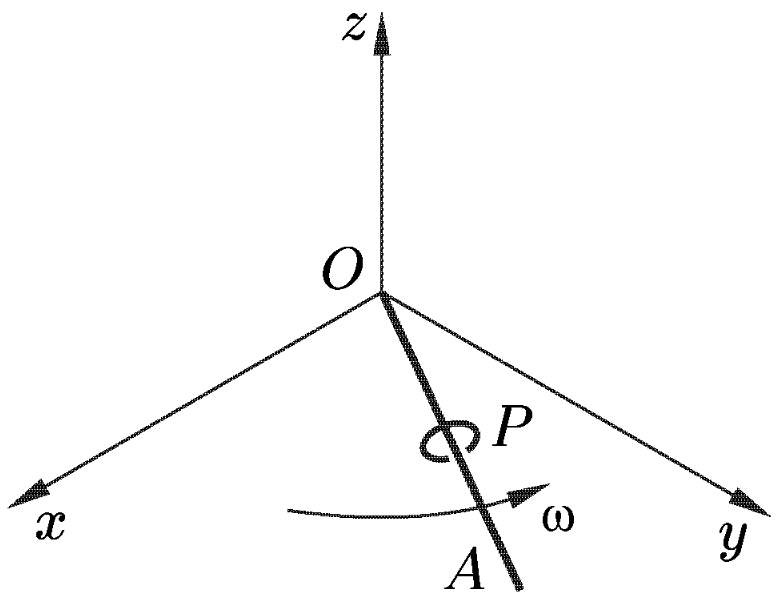
\includegraphics[width=0.24\textwidth]{img/2_15.png}
    \hspace{1cm} 
    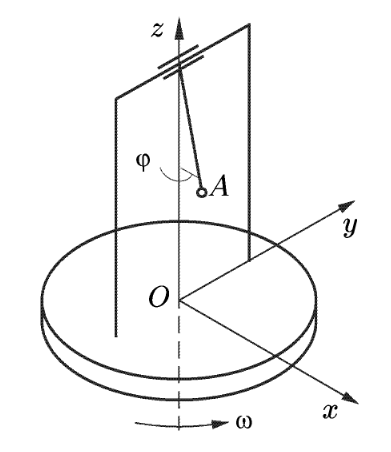
\includegraphics[width=0.2\textwidth]{img/2_19.png}
    \hspace{1cm} 
    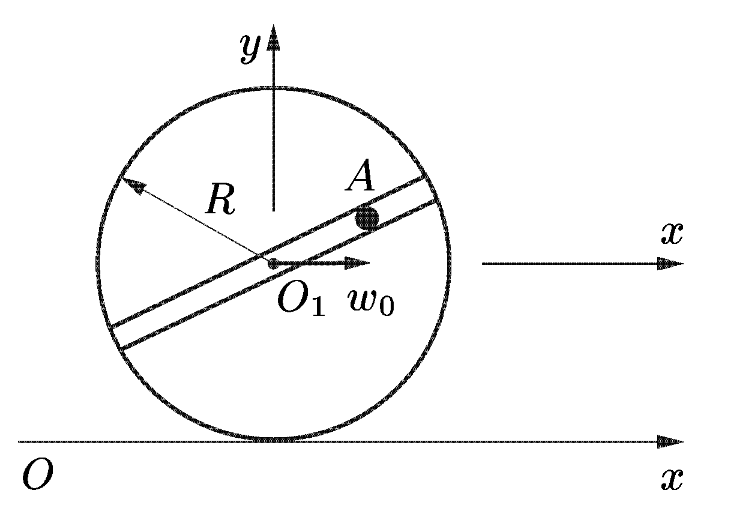
\includegraphics[width=0.3\textwidth]{img/2_35.png}
    \caption{Рисунки к задачам 2.15, 2.19 и 2.35.}
    %\label{fig:}
\end{figure}

\subsubsection*{2.19}

Для начала найдём и выразим все интересные нам векторы:
$$
    \left.\begin{aligned}
        \varphi         &= \varphi_0 \sin \omega_0 t            \\
        \dot{\varphi}   &= \varphi_0 \omega_0 \cos \omega_0 t   \\
        \ddot{\varphi}  &= - \varphi_0 \omega_0^2 \sin \omega_0 t \\
    \end{aligned}\right\},
    \vc{\mathrm{w}}_0 = - \begin{pmatrix}
        \omega^2 r \sin \varphi \\ 0 \\ 0
    \end{pmatrix},
    \vc{\omega}_m = \begin{pmatrix}
        0 \\ - \dot{\varphi} \\ 0
    \end{pmatrix},
    \vv{BA} = r \begin{pmatrix}
        \sin \varphi \\ 0 \\ - \cos \varphi
    \end{pmatrix},
    \vc{\varepsilon}^r = \begin{pmatrix}
        0 \\ -\ddot{\varphi} \\ 0
    \end{pmatrix},
$$

% \begin{wrapfigure}{r}{0.25\textwidth}
%   \begin{center}
%         \vspace{-5 mm}
%         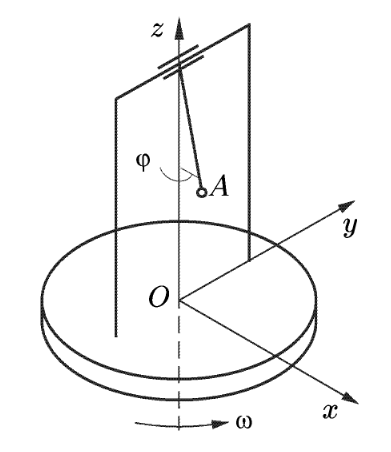
\includegraphics[width=0.8\linewidth]{img/2_19.png}
%   \end{center}
% \end{wrapfigure}

\noindent
где $\vc{\omega}_m$ -- угловая скорость $\vv{AB}$ относительно конструкции.

Во-первых, скорость $\vc{v}_A^a$ такая, что
$$
    \vc{v}_A^a = \vc{v}^e + \vc{v}^r = \vc{\omega} \times \vv{OA} + \vc{\omega}_m \times \vv{BA} =
    r \begin{pmatrix}
        \dot{\varphi} \cos \varphi \\ \omega \sin \varphi \\ \dot{\varphi} \sin \varphi,
    \end{pmatrix}
$$
а норма $\|\vc{v}_A^a\|$ в точке $t=t_0 = \pi / 2 \omega_0$ такая, что
$$
    \|\vc{v}_A^a\|^2 = r^2 \left(\dot{\varphi} + \omega^2 \sin^2 \varphi \right)
    \hspace{0.5cm} \Rightarrow \hspace{0.5cm} 
    \|\vc{v}_A^a\|^2 \bigg|_{t=t_0} = r^2 \omega^2 \sin^2 \varphi_0.
$$
Во-вторых, ускорение $\vc{\mathrm{w}}_A^a$ такое, что
$$
    \vc{\mathrm{w}}_A^a = \vc{\mathrm{w}}_0 + 0 + \vc{\omega} \times \vc{\omega} \times \vv{BA} + 2 \vc{\omega} \times \left(
        \vc{\omega}_m \times \vv{BA}
    \right) + \vc{\mathrm{w}}^r.
$$
Подставляя значения для $t=t_0$, получим, что
$$
    \vc{\mathrm{w}}_A^a =
    -r
    \begin{pmatrix}
        \omega^2 \sin \varphi_0 + \varphi_0 \omega_0^2 \cos \varphi_0 \\
        0\\
        \varphi_0 \omega_0^2 \sin \varphi_0
    \end{pmatrix}.
$$
Соответсвенно, норма ускорения точки $A$
\begin{align*}
        \|\vc{\mathrm{w}}_A^a\|^2 &= r^2(
        \omega^4 \sin^2 \varphi_0 + \omega^2 \omega_0^2 \varphi_0 \sin^2 \varphi_0 +
        \varphi_0^2 \omega_0^4 \cos^2 \varphi_0 + \varphi_0^2 \omega_0^4 \sin^2 \varphi_0
        ) = \\
        &=r^2(\omega^4 \sin^2 \varphi_0 + \omega^2 \omega_0^2 \varphi_0 \sin^2 \varphi_0
                + \varphi_0^2 \omega_0^4).
\end{align*}

%%%%%%%%%%%%%%%%%%%%%%%%%%%%%%%%%%%%%%%%%%%%%%%%%%%%%%%%%%%%%%%%%%%%%%%%%%%%%%%%%%
\subsubsection*{2.35}
%%%%%%%%%%%%%%%%%%%%%%%%%%%%%%%%%%%%%%%%%%%%%%%%%%%%%%%%%%%%%%%%%%%%%%%%%%%%%%%%%%

Снова предварительно запишем необходимые нам величины,
$$
\left.\begin{aligned}
    \vv{O_1A} = \vc{r}_A^r &= \vc{a} \sin \omega t, \\
    \vc{v}_A^r &= \vc{a} \omega \cos \omega t, \\
    \vc{\mathrm{w}}_A^r &= - \vc{a} \omega^2 \sin \omega t\\
\end{aligned}\right\}, \hspace{0.4cm} 
\vc{a} = a \begin{pmatrix}
    \cos \varphi \\ \sin \varphi \\ 0
\end{pmatrix}, \hspace{0.4cm} 
\varphi = - \frac{\vc{\mathrm{w}}_0 t^2}{2R},\hspace{0.4cm} 
\vc{v}_0 = \vc{\Omega} R = \vc{\mathrm{w}}_0 t,\hspace{0.4cm} 
\vc{\varepsilon} = \begin{pmatrix}
    0 \\ 0 \\ \mathrm{w}_0 / R
\end{pmatrix}.
$$
где $\varphi(t)$ и $\vc{\Omega}(t)$ мы знаем из условия $\vc{\mathrm{w}}_0 = \const$.

Скорость $\vc{v}_A^a$ такая, что
$$
    \vc{v}_A^a = \vc{v}_0 + \vc{\Omega} \times  \vc{r}_A^r 
    + \vc{v}_A^r 
    \hspace{0.5cm} \Rightarrow \hspace{0.5cm} 
    \left\{\begin{aligned}
        v_x &= \mathrm{w_0} t\left(
            R + a \sin \varphi \sin \omega t
        \right) / R + a \omega \cos \varphi \cos \omega t \\
        v_y &= a \omega \sin \varphi \cos \omega t - 
        \mathrm{w}_0 t a \cos \varphi \sin \omega t / R\\
        v_z &= 0 \\
    \end{aligned}\right.
$$
а норма 
$$
    \|\vc{v}_A^a\|^2 = \frac{\mathrm{w_0}^2 t^2}{R^2}  a^2 \sin^2 \omega t +
    a^2 \omega^2 \cos^2 \omega t +
    \mathrm{w}_0^2 t^2 +
    2 \frac{\mathrm{w_0}t}{R}a \left(
        \mathrm{w}_0 t \sin \varphi \sin \omega t + R \omega \cos \varphi \cos \omega t
    \right).
$$
или, преобразуя, получим, что
$$
    \|\vc{v}_A^a\|^2 = 
    \left(
        \frac{\mathrm{w}_0 t}{R} a \sin \omega t  \mathrm{w}_0 t \sin \varphi 
    \right)^2 + \left( \vphantom{\frac{1}{2}}
        a \omega \cos \omega t + w_0 t \cos \varphi
    \right)^2.
$$

Ускорение $\vc{\mathrm{w}}_A^a$ такое, что
$$
    \vc{\mathrm{w}}_A^a = 
    \vc{\mathrm{w}}_0 + \vc{\varepsilon} \times \vc{r}_A^r +
    \Omega \times \Omega \times \vc{r}_A^r +
    2 \vc{\Omega} \times \vc{v}_A^r + \vc{\mathrm{w}}^r_A.
$$
Подставляя значения, получим
$$
    \vc{\mathrm{w}}^c = \frac{1}{R} 
    \left(\begin{matrix}2 \omega a t \mathrm{w}_0 \sin{\left(\varphi \right)} \cos{\left(\omega t \right)}\\- 2 \omega a t \mathrm{w}_0 \cos{\left(\varphi \right)} \cos{\left(\omega t \right)}\\0\end{matrix}\right), \hspace{0.7cm} 
    % 
    \vc{\mathrm{w}}^e = \frac{1}{R^2} 
     \left(\begin{matrix}\mathrm{w}_0 \left(R^{2} + R a \sin{\left(\varphi \right)} \sin{\left(\omega t \right)} - a t^{2} \mathrm{w}_0 \sin{\left(\omega t \right)} \cos{\left(\varphi \right)}\right)\\- a \mathrm{w}_0 \left(R \cos{\left(\varphi \right)} + t^{2} \mathrm{w}_0 \sin{\left(\varphi \right)}\right) \sin{\left(\omega t \right)}\\0\end{matrix}\right).
$$
Суммруя, получим, что
$$
    \left\{\begin{aligned}
        \left(\vc{\mathrm{w}}_A^a\right)_x &= 
        \frac{1}{R^2} \left(
            R^{2} \left(- \omega^{2} a \sin{\left(\omega t \right)} \cos{\left(\varphi \right)} + \mathrm{w}_0\right) + R a \mathrm{w}_0 \left(2 \omega t \cos{\left(\omega t \right)} + \sin{\left(\omega t \right)}\right) \sin{\left(\varphi \right)} - a t^{2} \mathrm{w}_0^{2} \sin{\left(\omega t \right)} \cos{\left(\varphi \right)}
        \right) \\
    \left(\vc{\mathrm{w}}_A^a\right)_y &= 
    \frac{1}{R^2} \left(
        - a \left(R^{2} \omega^{2} \sin{\left(\varphi \right)} \sin{\left(\omega t \right)} + R \mathrm{w}_0 \left(2 \omega t \cos{\left(\omega t \right)} + \sin{\left(\omega t \right)}\right) \cos{\left(\varphi \right)} + t^{2} \mathrm{w}_0^{2} \sin{\left(\varphi \right)} \sin{\left(\omega t \right)}\right)
    \right) \\
    \left(\vc{\mathrm{w}}_A^a\right)_z &= 0.
    \end{aligned}\right.
$$



%%%%%%%%%%%%%%%%%%%%%%%%%%%%%%%%%%%%%%%%%%%%%%%%%%%%%%%%%%%%%%%%%%%%%%%%%%%%%%%%%%
\subsubsection*{4.14 и 4.15*}
%%%%%%%%%%%%%%%%%%%%%%%%%%%%%%%%%%%%%%%%%%%%%%%%%%%%%%%%%%%%%%%%%%%%%%%%%%%%%%%%%%

Сделаем задачу чуть менее абстрактной. Представим кольцевую железную дорогу, плоскость которой нормальна к $\vc{\omega}_1$. Наш агент  \textnumero 1 сидит в вагоне поезда и на столе, поверхность которого нормальна к $\vc{\omega}_2$, запускает игрушечную кольцевую жилезную дорогу с игрушечным агентом  \textnumero 2 в вагоне поезда. Агент  \textnumero 2 запускает поезд на столе, поверхность которого нормальна к $\vc{\omega}_3$ ...

Найдём $\vc{\varepsilon}_{\text{\textnumero} 2}$ -- угловое ускорение агента \textnumero 2. По словам \textnumero 1, угловое ускорение равно $\vc{\omega}_{\text{\textnumero 2}} = \vc{\omega}_2$, тогда
$$
    \vc{\varepsilon}_{\text{\textnumero} 2} = \underbrace{\vc{\varepsilon}_1}_{\vc{\varepsilon}^e} + \frac{d}{dt} \vc{\omega}_2 = 0 + 
    \frac{\vc{\omega}_2}{\omega_2} \dot{\omega}_2
    + 
    \vc{\omega}_1 \times \vc{\omega}_2.
$$
А теперь найдём $\vc{\varepsilon}_3$. С точки зрения \textnumero 2 $\vc{\omega}_{\text{\textnumero 3}} = \vc{\omega}_3$. Мы знаем, что $\vc{\omega}_{\text{\textnumero 2}} = \vc{\omega}_1 + \vc{\omega}_2$, и знаем $\vc{\varepsilon}_{\text{\textnumero} 2}$, тогда
$$
    \vc{\varepsilon}_{\text{\textnumero} 3} = \vc{\varepsilon}_2 + \frac{d}{dt} \vc{\omega}_3 = 
    \left(\frac{\vc{\omega}_2}{\omega_2} \dot{\omega}_2 + \vc{\omega}_1 \times \vc{\omega}_2\right)
    + 
    \frac{\vc{\omega}_3}{\omega_3} \dot{\omega}_3
    + 
    (\vc{\omega}_1 + \vc{\omega}_2) \times \vc{\omega}_3.
$$
И так далее мы можем продолжать добавлять вектора $\vc{\omega}_i$ к движению тела, в силу $\vc{\omega}^a = \vc{\omega}^e + \vc{\omega}^r$, при чём мы получим слагаемые вида векторного произведение всех упорядоченных пар $\vc{\omega}_j$ и $\vc{\omega}_k$, плюс сумма $\vc{\varepsilon}^r_i$.
$$
    \vc{\varepsilon}_{\text{\textnumero} N} = \vc{\varepsilon}_{\text{\textnumero} (N-1)} + 
    \frac{\vc{\omega}_N}{\omega_N} \dot{\omega}_N +
    \vc{\omega}_{\text{\textnumero} (N-1)} \times \vc{\omega}_N.
$$
По индукции можем показать, что
$$
    \vc{\varepsilon} = \vc{\varepsilon}_{\text{\textnumero} N} = \sum_{j=2}^n \frac{\vc{\omega}_j}{\omega_j} \dot{\omega}_j + \sum_{k=2}^N \sum_{i=1}^{k-1} \vc{\omega}_i \times \vc{\omega}_k.
$$
В частности, при $\dot{\omega}_j = 0$, получим выражение для задачи \textbf{4.14}.


%%%%%%%%%%%%%%%%%%%%%%%%%%%%%%%%%%%%%%%%%%%%%%%%%%%%%%%%%%%%%%%%%%%%%%%%%%%%%%%%%%%
\subsubsection*{Т9.*}


\begin{wrapfigure}{r}{0.2\textwidth}
  \begin{center}
      \vspace{-50mm}
        \incfig{1}    
  \end{center}
\end{wrapfigure}

Рассмотрим движение выпуклого твёрдого тела по выпуклой поверхности. Они соприкасаются в точках $A$ и $C$ соответсвенно. Пусть есть некоторая неподвижная СО, относительно начала которой будем записыввать радиус векторы. Пусть точка $O$ -- мгновенный центр скоростей, тогда скорость некоторой точки тела может быть найдена, как
$$
    \vc{v} = \vc{\omega} \times \left(
        \vc{r} - \vc{r}_O
    \right),
$$
где $\vc{r}$ -- радиус вектор этой точки.

Для точки $A$ верно, что $\vc{v}_A = \vc{\omega} \times \left(\vc{r}_A - \vc{r}_O\right) = 0$, дифференцируя равенство по времени, найдём, что
$$
    \vc{\mathrm{w}}_A = \vc{\dot{\omega}} \times \underbrace{\left(\vc{r}_A - \vc{r}_O\right)}_{= 0} + \vc{\omega} \times \frac{d}{dt} \left(\vc{r}_{A}- \vc{r}_O\right) =
    - \vc{\omega} \times \vc{\dot{r}}_O,
$$
где $\vc{r}_A - \vc{r}_O = 0$, т.к. тело движется без проскальзывания и в данный момент времени $A$ соответсвует мгновенному центру скоростей.
Рассматривая движение относительно центра кривизны $B$, поймём, что $\vc{v}_C = \vc{v} = \vc{v}_O = \vc{\dot{r}}_O$, получается, $\vc{\mathrm{w}}_A = - \vc{\omega} \times \vc{v}$, Q.E.D.




\section{Динамика I}
\setcounter{subsection}{4}
\subsection{Основные теоремы динамики}

\subsubsection*{5.10}

Парметризуем систему движением по оси $z \parallel \vc{g}$, тогда
\begin{equation}
    m \dot{v} = \beta v^2 - mg \frac{R^2}{(R+z)^2}.
\end{equation}
Что аналогично диф. уравнению
\begin{equation}
    \ddot{z} = \frac{\beta}{m} \dot{z}^2 - g \frac{R^2}{(R+z)^2} .
\end{equation}
Решим диф. уравнение заменой $\dot{z} = p(v) \equiv v$, тогда $\ddot{z} = p'p$.
Пусть теперь $y = v^2$, $x'/2 = p'p$, тогда приходим к однородному диф. уравнению
\begin{equation}
    \frac{1}{2} y' - \frac{\beta}{m} x = \frac{-gR^2}{(R+z)^2}.
\end{equation}
Решая, получим, что
\begin{equation}
    C(z) = -2g \int \left(1 + \frac{z}{R} \right)^{-2} \exp\left(-\frac{2\beta}{m} z\right) \d z + C_0.
\end{equation}
Из начальных условия  находим $C_0$, получая
\begin{equation}
    v^2 = v_0^2 \exp\left(-\frac{2\beta}{m} \left(H-h\right)\right)
    -2gR^2 \exp\left(\frac{2\beta}{m} h\right)
    \int_{H}^{h} \left(R+z\right)^{-2} \exp\left(-\frac{2\beta}{m} z\right)\d z.
\end{equation}

%%%%%%%%%%%%%%%%%%%%%%%%%%%%%%%%%%%%%%%%%%%%%%%%%%%%%%%%%%%%%%%%%%%%%%%%%%%%%%%%%%%

\subsubsection*{6.13}

Из теоремы об изменение количества движения, ц.м. системы покоится. Т.к. на систему не действуют внешние силы с ненулевым относительно вертикальной оси моментом, то по теореме об изменение кин. момента, он сохраняется $K_0 = K_1$. 

Далее всё запишем  в проекции на вертикальную ось. В начальный момент времени
\begin{equation} 
     K_0 = I \omega_0 = \frac{3}{10} k m r^2 \omega_0.
 \end{equation} 
При достижении шариком пола
\begin{equation}
    K_1 = I'\omega' + m (kl)^2 \omega'.
\end{equation}
По т. Штейнера
\begin{equation}
    I'\omega' = I \omega' + kml^2 = \frac{3}{10} kmr^2 \omega' + kml^2\omega'.
\end{equation}
Собирая всё вместе получаем, что
\begin{equation}
    3k (k+1) \omega_0 = \left(
        3k(k+1) + 10k
    \right) \omega'
    \hspace{0.5cm} \Rightarrow \hspace{0.5cm} 
    \boxed{
        \omega'= \frac{3(k+1)}{3k + 13} \omega_0
    }
\end{equation}


%%%%%%%%%%%%%%%%%%%%%%%%%%%%%%%%%%%%%%%%%%%%%%%%%%%%%%%%%%%%%%%%%%%%%%%%%%%%%%%%%%%

\subsubsection*{6.25}

Кинетический момент 
\begin{equation}
    \frac{d}{dt} \vc{K}_A = \vc{M}_A^e + \vc{Q} \times \vc{v}_A,
\end{equation}
где $A$ -- мгновенный центр скоростей, $\vc{v}_A = 0$. Тогда, в проекции на вертикальную ось, получим, что
\begin{equation}
    \frac{d}{dt} \vc{K}_A = \vc{M}_A^e = \vc{l} \times \vc{F}_{\text{тр}}
    \hspace{0.5cm} \Rightarrow \hspace{0.5cm} 
    \vc{K}_A\big|_z = \const.
\end{equation}


%%%%%%%%%%%%%%%%%%%%%%%%%%%%%%%%%%%%%%%%%%%%%%%%%%%%%%%%%%%%%%%%%%%%%%%%%%%%%%%%%%%

\subsubsection*{6.35}
Для точек пластины $\vc{r}_{AC} = \vc{r}_C - \vc{r}_A$, $\vc{v}_i = \vc{v}_A + \vc{\omega} \times \vc{r}_{Ai}$. Соответственно
\begin{equation}
    \vc{K}_A = \sum_i \vc{r}_{Ai} \times m_i \left(
        \vc{v}_A + \vc{\omega} \times \vc{r}_Ai
    \right) =
    \vc{v}_A \times \sum_i \left(\vc{r}_A - \vc{r}_i\right) m_i
    +
    \sum_i \vc{r}_{Ai} \times (m_i \vc{\omega} \times \vc{r}_{Ai}).
\end{equation}
Раскрывая по правилу Лагранжа, получим, что
\begin{equation}
    \vc{K}_A = m \left(
        \vv{AC} \times \vc{v}_A
    \right) + I_A \vc{\omega},
    \hspace{0.5cm} 
    \text{Q.E.D.}
\end{equation}


%%%%%%%%%%%%%%%%%%%%%%%%%%%%%%%%%%%%%%%%%%%%%%%%%%%%%%%%%%%%%%%%%%%%%%%%%%%%%%%%%%%
\subsubsection*{7.4}
Во-первых запишем кинетическую энергию системы, как
\begin{equation}
    T_{\text{сист}} = T_{\text{диска}} + T_{\text{стержня}}.
\end{equation}
Начнем с простого,
\begin{equation}
    T_{\text{ст}} = \frac{1}{2} \left(
        M \frac{l^2}{3} \omega^2
    \right).
\end{equation}
Точка $K$ -- мгновенный центр скоростей, то
\begin{equation}
    \vc{v}_d = \vc{\omega} \times \vc{l} = \vc{\omega}_d \times \vc{r}
    \hspace{0.5cm} \Rightarrow \hspace{0.5cm} 
    \omega_d = \omega \frac{l}{r}.
\end{equation}
Аналогично для обруча
\begin{equation} 
    \vc{v}_{\text{об}} = \vc{\omega}_{\text{об}} \times \vc{\rho} = \vc{\omega} \times \vv{OB}
    \hspace{0.5cm} \Rightarrow \hspace{0.5cm} 
    \omega_{\text{об}} = \omega \frac{R-\rho}{\rho} .
\end{equation}
Теперь можем записать для диска 
\begin{equation}
    T_{\text{д}} = \frac{1}{2} I_d \omega_d^2 + \frac{mv_0^2}{2} =
    \frac{3}{4} m \omega^2 l^2.
\end{equation}
И, наконец, для обруча,
\begin{equation}
    T_{\text{об}} = \frac{1}{2} \mu \omega^2 (R-\rho) + \frac{1}{2} \mu \rho^2 \omega^2 \frac{(R-\rho)^2}{\rho^2} = \mu (R-\rho)^2 \omega^2.
\end{equation}
Собирая всё вместе, получим
\begin{equation}
    \boxed{
        T = \omega^2
        \left(
            \mu \left(l+r-\rho\right)^2 + \frac{3}{4} m l^2 + \frac{1}{6} M l^2
        \right)
    }
\end{equation}


\subsubsection*{7.12}

Изначально, известно, что
\begin{equation}
    \left\{\begin{aligned}
        F_x &=  yz \sin \omega t\\
        F_y &= x z \sin \omega t\\
        F_z &= xy \sin \omega t\\
    \end{aligned}\right.
\end{equation}
Проверим, что поле потенциально
\begin{equation}
    \rot \vc{F} = 0.
\end{equation}
Да, действитеьно потенциально. Тогда выбрав в качетсве $0$ потенциальной энергии $U$ нулевой момент времени, получим
\begin{equation}
    U = \int_{x_0}^{x} F_x \d x +
    \int_{y_0}^{y} F_y \d y +
    \int_{z_0}^{z} F_z \d z
    \hspace{0.5cm} \Rightarrow \hspace{0.5cm} 
    \boxed{
        U = xyz \sin \omega t
    }
\end{equation}

\subsubsection*{9.11}

Точка $A$ подвеса математического маятника длины $l$ совершает вертикальные колебания по закону
$$
    \vv{OA} = \vc{a} \sin (\omega t) = \vc{r}_A,
    \hspace{0.5cm} 
    \vc{a} \omega \cos (\omega t) = \vc{v}_A,
    \hspace{0.5cm} 
    - \vc{a} \omega^2 \sin (\omega t) = -\vc{\mathrm{w}}^e.
$$
Тогда по II закону Ньютона для неИСО
\begin{equation}
    m \vc{\mathrm{w}}^r = \vc{F} + m \vc{g} - m \vc{\mathrm{w}}^e.
\end{equation}
Пусть ось $OX$ противонаправлена силе натяжения нити $\vc{F}$, $OY$ в плоскости движения, тогда, введём $\vc{g}' = \vc{g}-\vc{\mathrm{w}}^e$ и получим
\begin{align*}
    &OX: \ \  m \mathrm{w}_x = - F + m g' \cos \varphi  = 0,\\
    &OY: \ \  m \mathrm{w}_y = mg' \sin \varphi,
\end{align*}
Так приходим к уравнению вида
\begin{equation}
    \ddot{\varphi} +  \frac{1}{L} \left(
    \vphantom{\frac{1}{2} }
        g - a \omega^2 \sin \left(\omega t\right)
    \right) \sin (\varphi)= 0.
\end{equation}
В частности, заметим, что $\varphi(t)\equiv0$ и $\varphi(t) \equiv \pi$ являются частными решениями этого уравнения.

\subsubsection*{9.16}

Невесомый стержень вращается с постоянной угловой скоростью $\vc{\omega}$ вокруг оси $Oz$, перпендикулярной плоскости рисунка. По диску катится диск радиуса $r$ и массы $m$, в начальный момент точки $O$ и $A$ совпадали, а диск покоился.

Перейдём в СО стержня, тогда 
\begin{equation}
    m\vc{\mathrm{w}}_d^r =
     m\vc{\mathrm{w}}_d^a - m\vc{\mathrm{w}}_d^c - m\vc{\mathrm{w}}_d^e.
\end{equation}
Так как движение происходит без проскальзывания, сила трения не совершает работу. С учётом II закона Ньютона в неИСО, и тем что сила Кориолиса не изменяет кинетическую энергию системы, получим, что внешний момент
\begin{equation}
    \vc{M}_i = \vc{R}_i \times \left(
        m_i \vc{g} 
        - 
        m_i \vc{\omega} \times \vc{\omega} \times \vc{r}_i
    \right),
    \hspace{0.5cm} 
    \vc{r}_i = \vv{OA} + \vc{R}_i,
\end{equation}
Тогда
$$
    \vc{M}_i =
    m_i \vc{R}_i \times \vv{OA} \omega^2 -
    m_i \vc{R}_i \times \vc{\omega} \left(\vc{\omega} \cdot \vv{OA}\right) + m_i \vc{R}_i \times \vc{g},
$$
Суммируя, по теореме об изменение кинетического момент, получим, что
$$
    I \vc{\varepsilon}_d = \sum \vc{M}_i = m \omega^2  \ \vv{AB} \times \vv{OA} + m \ \vv{AB} \times \vc{g}.
$$
Пусть $L$ -- пройденное расстояние, в проекции на ось, сонаправленную с $\vc{\omega}_d^r$,
$$
    \frac{d \omega_d^r}{dt} =
    \frac{2}{3} \frac{L}{R} \omega^2 + \frac{2}{3} \frac{g}{R} \cos \varphi,
$$
интегрируя, с учётом начальных условий,
\begin{equation}
    (\omega_d^{r})^2 (L) =
    \frac{2}{3} \frac{L^2}{R^2} \omega^2 + \frac{4}{3} \frac{L}{R^2} \, g \cos \varphi.
\end{equation}

Запишем теперь Кориолисову силу, как
$$
    \vc{F}^c_i = - 2 \omega \times (\vc{\omega} \times \vc{r}_i) m_i
    \hspace{0.5cm} \Rightarrow \hspace{0.5cm} 
    \vc{F}^c = - 2 \vc{\omega} \times
    \left(
        \vc{\omega}_d^r \times \vv{AB} 
    \right) \ m.
$$
Догда записав II закон Ньютона на ось, сонаправленную с $\vc{N}$, получим
\begin{equation}
    0 = N - mg\sin\varphi - R m \omega^2  + 2 m \omega \omega_d^r R
    \hspace{0.5cm} \Rightarrow \hspace{0.5cm} 
    {
        N = mg \sin \varphi + Rm \omega^2-
        2 m\omega \sqrt{
            \frac{2}{3} \omega^2 L^2 + \frac{4}{3} g L \cos \varphi 
        }
    }    
\end{equation}
Аналогично записав уравнение в проекции на ось, сонаправленную с $\vc{F}_\text{тр}$, найдём
\begin{equation}
    m {\mathrm{w}} = m \varepsilon R = F_{\text{тр}} + L m \omega^2 + mg \cos \varphi,
    \hspace{0.5cm} \Rightarrow \hspace{0.5cm} 
    {
        F_{\text{тр}} = \frac{m}{3} \left(
            \vphantom{\frac{1}{2}}
            L\omega^2 + g \cos \varphi
        \right)
    }.
\end{equation}



\subsubsection*{9.27}
Посмотрим на систему с точки зрения вращающейся с угловой скоростью $\vc{\omega}_0$ плоскости, тогда по теореме об изменение количества движения в неИСО
\begin{equation}
    m \vc{\mathrm{w}}^r = \vc{R} - m \vc{\mathrm{w}}^e - m \vc{\mathrm{w}}^c.
\end{equation}
Выберем в качестве полюса тела центр масс $A$, тело вращается относительно него с $\vc{\omega}$, тогда 
$$
    - \frac{1}{2} \vc{F}^C  = 
    \sum_i m_i \left(
        \vc{\omega}_0 \times (\vc{v}_A + \vc{\omega} \times \vv{Ci})
    \right) = m \vc{\omega}_0 \times \vc{v}_A +
    \vc{\omega}_0 \times \left(
        \vc{\omega} \times \big(
        \cancel{\sum m_i \vc{r}_i}
        \big)
    \right) = m \vc{\omega}_0 \times \vc{v}_A.
$$
Аналогично для переносной
$$
    -\vc{F}^e = \sum m_i \vc{\omega} \times \vc{v}_i^r =
    \sum_i m_i \vc{\omega} \times \vc{\omega} \times \vc{r}_i =
    \vc{\omega} \times \vc{\omega} \times \left(
        \sum_i m_i \vc{r}_i
    \right) = m \vc{\omega} \times \left(\vc{\omega} \times \vc{r}_A\right).
$$
Таким образом переносные и кориолисовы силы приводятся к равнодействующим, проходящим через центр масс фигуры.
% \subsubsection*{9.32}

% Шарик движется так, что скорость всех его точек параллельны плоскости, которая вращается с угловой скоростью $\omega(t)$ вокруг неподвижной оси, лежащей вэтой плоскости. 

% В плоскости введем координаты так, что
% $$
%     \vc{\omega} = \begin{pmatrix}
%         0 \\ 0 \\ \omega
%     \end{pmatrix},
%     \hspace{0.5cm} 
%     \vc{a} = \begin{pmatrix}
%         \sin \omega t \\
%         \cos \omega t \\
%         0
%     \end{pmatrix},
%     \vc{v} = \begin{pmatrix}
        
%     \end{pmatrix}
% $$
 %-
\subsection{Движение точки в центральном поле сил}


\subsubsection*{8.21}

В приближении $m \ll M$, запишем, что
$$
    \vc{F}(r) = \frac{kQq}{r^2} \frac{\vc{r}}{r} = \varepsilon u^2 \frac{\vc{r}}{r},
$$
% Для такого движения мы знаем, что
% $$
%     \frac{1}{u} = r = \frac{p}{1 - e \cos \varphi}.
% $$
В силу того, что $\dot{\varphi} = cu^2$, то из момента, когда $\dot{\varphi} = v_0 / r$, найдём $c=v_0 d$.
Уравнение Бине примет вид
\begin{equation}
    u'' + u = \frac{kQq}{mv_0^2 d^2} 
    \overset{\mathrm{def}}{=} \varkappa.
\end{equation}
При $\varphi \to 0$, получим, что
$$
    u_0 \cos \varphi_0 = -\varkappa.
$$
Дифференцируя же по времени, получим
$$
    \dot{u} = - u_0 \sin (\varphi - \varphi_0) \dot{\varphi}
    \hspace{0.5cm} \Rightarrow \hspace{0.5cm} 
    \dot{r} = u_0 v_0 d \sin \left(\varphi - \varphi_0\right),
$$
Таким образом
$$
    \left\{\begin{aligned}
        u_0 &= 1 / d \sin \varphi_0 \\
        u_0 &= - \varkappa  \cos \varphi_0
    \end{aligned}\right. ,
    \hspace{0.5cm} \Rightarrow \hspace{0.5cm} 
    \tg \varphi_0 = - \frac{1}{\kappa d}.
$$
Теперь при $u \to 0$, получим
$$
    \theta' - \varphi_0 = \arccos \left(\frac{-\varkappa}{u_0} \right),
    \hspace{0.5cm} \Rightarrow \hspace{0.5cm} 
    \theta = \pi - \theta = \pi - 2 \arctg \frac{1}{\varkappa d} 
    =
    2 \arctg \left(\varkappa d\right),
$$
Таким образом приходим к выражению
\begin{equation}
    \theta = 2 \arctg \left(\varkappa d\right).
\end{equation}

\subsubsection*{Т10*.}

В ОТО движение в центральном поле тяжести описывается как движение в метрике Шварцшильда:
$$
    d s^2 = \left(1 - \frac{a}{r} \right) \d \tau^2
    -
    \left(1 - \frac{a}{r} \right)^{-1} \d r^2
    -
    (r \sin \theta)^2 \d \varphi^2 - r^2 \d \theta^2.
$$
Здесь 4 независимых переменных $(\tau, r,  \varphi, \theta)$, где три из сферических координат, а $\tau$ -- физическое время,
также введен радиус Шварцшильда $a = 2 GM$.

Движение точек рассматриваем, как движение по геодезическим, то есть $\vc{\mathrm{w}}_i = 0$, где $i \in \{\tau, r, \varphi, \theta\}$. Движение будет в некотором смысле происходить в одной плоскости, так что пусть $\theta (t) = \pi / 2$. Так мы получим следующую систему уравнений:
\begin{equation}
    \left\{
        \begin{aligned}
            v^2 &= 
            \left(
            \frac{ds}{dt} \right)^2 = \left(1 - \frac{a}{r} \right) \dot{\tau}^2
            - \left(1 - \frac{a}{r} \right)^{-1} \dot{r}^2 - r^2 \dot{\varphi}^2 \\
            \vc{\mathrm{w}}_\tau &=
            \frac{d}{dt} \frac{\partial (v^2/2)}{\partial \dot{\tau}} -
            \underbrace{\frac{\partial (v^2/2)}{\partial \tau}}_{0} =
            \frac{d}{dt} \left[\left(
                       1 -  \frac{a}{r} 
                    \right) \dot{\tau}\right] = 0 \\
            \vc{\mathrm{w}}_\varphi &= 
            - \frac{d}{dt} \left[
                r^2 \dot{\varphi}
            \right] = 0
        \end{aligned}
    \right.
\end{equation}
Таким образом получим пару первых интегралов системы, в частности
\begin{align*}
    \left(1 - \frac{a}{r} \right) \dot{\tau} &= \mathcal D,
    \\ r^2 \dot{\varphi} &= \mathcal C.
\end{align*}
Подставляя их в выражение для скорости, получим, что
\begin{equation*}
\left(
1 - \frac{a}{r} 
\right)^{-1} \mathcal D^2 -
\left(1 - \frac{a}{r} \right)^{-1} \dot{\vc{r}}^2 - \frac{c^2}{r^2}  = v^2.
\end{equation*}
По замене Бине 
$$
    r = \frac{1}{u}, \hspace{0.5cm} 
    \dot{r} = r' \dot{\varphi} = \left(\frac{1}{u} \right)' c u^2 =
    - u' c,
$$
перейдём к функции $u(\varphi)$:
\begin{equation}
    2 c^2 u'' + c^2 (2u - 3 au^2) = v^2.
\end{equation}
Преобразуя, получим
\begin{equation}
\boxed{
    u'' + u = \frac{a}{2c^2} v^2 + \frac{3}{2} au^2
}.
\end{equation}


Найдём теперь видимый радиус черной дыры -- минимальное значение прицельного параметра, при котором луч, проходящий через окрестность черной дыры не падает на центр. Для светового луча верно, что $\dot{s}^2=v^2=0$, тогда
$$
    u'' + u = \frac{3}{2} a u^2.
$$
Интегрируя, получим
$$
    \frac{u'^2}{2} + \frac{u^2}{2} = \frac{au^3}{2} + c'.
$$
Посмотрим теперь на поведение света при $u \to 0$ верно, что $r\varphi \to b$, тогда 
$$
    \frac{dr}{d\varphi} = - \frac{r}{\varphi} 
    \hspace{0.5cm} \Rightarrow \hspace{0.5cm} 
    \frac{du}{d\varphi} = - \frac{dr}{d\varphi} \frac{1}{r^2} = \frac{r}{\varphi} \frac{1}{r^2} = \frac{1}{r \varphi}
    \hspace{0.5cm} \Rightarrow \hspace{0.5cm} 
    u'\big|_{t=0} = \frac{1}{b} 
    \hspace{0.5cm} \Rightarrow \hspace{0.5cm} 
    c' = \frac{1}{2b^2} 
$$
Переписав, получим
$$
    u'^2 = au^3 - u^2 + \frac{1}{b^2}.
$$
Вблизи точки с критическим $u$ верно, что $\dot{r} \sim 0$, тогда нас интересует экстремум функции $au^3 - u^2 + b^{-2}$, тогда
$$
    3 a u^2 - 2 u = 0
    \hspace{0.5cm} \Rightarrow \hspace{0.5cm} 
    \frac{1}{r_{\text{min}}} = \left(\frac{3}{2} a\right)^{-1}.
$$
Условие падения -- уменьшение радиуса (увеличиение $u$) при $r=r_{\text{min}}$:
$$
    u'^2_{\text{min}} = \frac{1}{a^2} \left(
        \frac{8}{27} - \frac{4}{9} 
    \right) + \frac{1}{b^2} =
    -\frac{4}{27a^2}  + \frac{1}{b^2}  \geq 0
    \hspace{0.5cm} \Rightarrow \hspace{0.5cm} 
    b^2 \leq \frac{27}{4} a^2
$$
Тогда минимальное значение прицельного параметра, при котором луч, проходящий через окрестность черной дыры не падает на центр
\begin{equation}
    \boxed{b_{\text{min}} = \frac{3\sqrt{3}}{2} a},
\end{equation}
что и является видимым радиусом черной дыры.
\subsection{Элементы механики сплошых сред (МСС)}


\subsubsection*{Т14*.}

Хотелось бы выразить лапласиан $\Delta p$ через частные производные в произвольной криволинейной системе координат. Легко показать, что
\begin{equation}
    \Delta p = \div \grad f.
\end{equation}
Так что начнём с вида $\div \vc{v}$ и $\grad f$ в криволинейной системе координат. Понадеемся, что достаточно рассмотреть случай кривольнейных координат, орбазующих ортогональный базис в каждой точке пространства. 

В криволинейных координатах базисные направления сформированы векторами $\vc{g}_i (\vc{r}) \overset{\mathrm{def}}{=} \partial \vc{r} / \partial q^i$. Для удобства введём единичные орты координатных направлений для ортогональной системы
\begin{equation}
\label{b1}
    \vc{e}_1 (q) = \left(
        \frac{1}{\sqrt{g_{11}}}, 0, 0
    \right), \hspace{0.5cm} 
    \vc{e}_2 (q) = \left(
        0, \frac{1}{\sqrt{g_{22}}}, 0
    \right), \hspace{0.5cm} 
    \vc{e}_3 (q) = \left(
        0, 0, \frac{1}{\sqrt{g_{33}}}
    \right).
\end{equation}
Тогда
\begin{align}
\label{b2}
    d q^j (\vc{e}_i) = \frac{1}{\sqrt{g_{ii}}} \delta^i_j,
    \hspace{0.5cm} 
    dq^i \wedge d q^j (\vc{e}_k, \vc{e}_l) = \frac{1}{\sqrt{g_{ii} g_{jj}}} \delta^{i}_{k} \delta^j_l.
\end{align}


Известно, что градиент функции соответсвует дифференциальной 1-форме. 
Её (по вектору $\vc{A}$) можно записать как $\omega^1_{A} = a_i \d q^i$.
С учётом введеного базиса можно записать, что 
$ \vc{A} = A^i \vc{e}_i, \; \forall \vc{A} \in T \mathbb{R}_q^3. $
Из \eqref{b2} получим, что
$$
    \omega^1_A (\vc{e}_i) = (\vc{A} \cdot \vc{e}_i) = A^i = \frac{a_i}{\sqrt{g_{ii}}},
$$
следовательное $a_i = A^i \sqrt{E_i}$, и, соответсвенно
\begin{equation}
    \omega^1_A = A^i \sqrt{g_{ii}} dq^i.
\end{equation}
Аналогично, пусть теперь $\grad f = A^i \vc{e}_i$. По определению
$$
    \omega^1_{\grad f} = d \omega_f^0 = d f = \frac{\partial f}{\partial q^i} d q^i.
    \hspace{0.5cm} \Rightarrow \hspace{0.5cm} 
    \boxed{
        \grad f = \frac{1}{\sqrt{g_{ii}}}  \frac{\partial f}{\partial q^i} \vc{e}_i.    
    }
$$

Теперь найдём $\div \vc{B}$, как дифференциальную 3-форму. Для начала поймём, что для вектора $\vc{B} (q) = (B^i \vc{e}_i) (q)$ форма
\begin{equation}
\label{wb2}
    \omega^2_{B} = b_1 dq^2 \wedge dt^3 + b_2 dq^3 \wedge dt^1 + b_3 dq^1 \wedge dt^2
\end{equation}
имеет следующий вид:
$$
    \omega^2_B (\vc{e}_2, \vc{e}_3) = (\vc{B}, \vc{e}_2, \vc{e}_3) = B^1.
$$
С другой стороны, из \eqref{b2} и \eqref{wb2},
$$
    \omega^2_B (\vc{e}_2, \vc{e}_3) =
    b_1 dq^2 \wedge dq^3 (\vc{e}_2, \vc{e}_3) = \frac{b_1}{\sqrt{g_{22} g_{33}}}.
$$
Получаем, что $b_1 = B^1 \sqrt{g_{22} g_{33}}$, аналогично можем получить, что
$b_2 = B^2 \sqrt{g_{11} g_{33}}$, $b_3 = B^3 \sqrt{g_{11} g_{22}}$.

Теперь, из определения, получаем
$$
    \omega^3_{\div B} = d \omega^2_B = 
    \left(
    \frac{\partial \sqrt{g_{22} g_{33}} B^1}{\partial q^1} +
    \frac{\partial \sqrt{g_{33} g_{11}} B^1}{\partial q^2} +
    \frac{\partial \sqrt{g_{11} g_{22}} B^1}{\partial q^3}
    \right)
    dq^1 \wedge dq^2 \wedge dq^3.
$$
Тогда
\begin{equation}
    \div \vc{B} = \frac{1}{\sqrt{\det g}} 
    \left(
        \frac{\partial \sqrt{g_{22} g_{33}} B^1}{\partial q^1} +
        \frac{\partial \sqrt{g_{33} g_{11}} B^1}{\partial q^2} +
        \frac{\partial \sqrt{g_{11} g_{22}} B^1}{\partial q^3} 
    \right)
\end{equation}

Собирая всё вместе получаем, что
\begin{equation}
    \Delta f = \div
    \left(
        \frac{1}{\sqrt{g_{ii}}}  \frac{\partial f}{\partial q^i} \vc{e}_i
    \right) =
    \frac{1}{\det g} 
    \underset{P(i,g,k)=1}{\sum_{i \neq j \neq k}^3}
    \left(
        \frac{\partial }{\partial q^i} \left[
            \sqrt{\frac{g_{jj} g_{kk}}{g_{ii}} } \frac{\partial f}{\partial q^i} 
        \right] 
    \right).
\end{equation}

В частности, для полярных
$$
    g_{ij} = \diag\left(1, r^2, 1\right)
    \hspace{0.5cm} \Rightarrow \hspace{0.5cm} 
        \Delta f = \frac{1}{r} \frac{\partial }{\partial r} 
    \left(r \frac{\partial f}{\partial r} \right) +
    \frac{1}{r^2} \frac{\partial^2 f}{\partial \varphi^2}  + \frac{\partial^2 f}{\partial z^2} .
$$


\section{Контрольная работа I}

% \subsection*{Задача №1}
Введём координаты так, чтобы $OX \parallel \omega$, и $OY \parallel \vv{OO}_1 \equiv \vc{l}$. Запишем скорость точки $O_1$ двумя способами
\begin{equation}
    \vc{v}_{O_1} = \vc{\omega} \times \vc{l} =
    \vc{\omega}_0 \times \vc{r}.
\end{equation}
Скорость точки $B$
$$
    \vc{v}_B^r = 2 \vc{\omega}_0 \times \vc{r},
$$
Ускорение точки $B$
\begin{equation}
    \vc{\mathrm{w}}_B^a
    =
    \vc{\mathrm{w}}_B^r 
    +
    \vc{\mathrm{w}}_B^e
    +
    \vc{\mathrm{w}}_B^c. 
\end{equation}
Что ж, по порядку
\begin{align*}
    \vc{\mathrm{w}}_B^r  
    &=
    2 \vc{\omega}_0 \times \left(
        \vc{\omega}_0 \times \vc{r}
    \right)
    = 
    \begin{pmatrix}
        - \omega_0^2 r& 0& 0
    \end{pmatrix}\T,
    \\
    \vc{\mathrm{w}}_B^e 
    &=
    \vc{\omega} \times \left(\vc{\omega} \times \vc{l}\right) 
    = 
    \begin{pmatrix}
        0& -\omega^2 l& 0
    \end{pmatrix}\T,
    \\
    \vc{\mathrm{w}}_B^c
    &= 2 \vc{\omega} \times \vc{v}_B^r =
    4 \vc{\omega} \times \left(\vc{\omega}_0 \times \vc{r}\right)
    = 
    \begin{pmatrix}
        0& -4\omega\omega_0 r& 0
    \end{pmatrix}\T,
\end{align*}
где подразумевается, что
$$
    \omega = \begin{pmatrix}
        \omega \\ 0 \\ 0
    \end{pmatrix}, \hspace{0.5cm} 
    \omega_0 = \begin{pmatrix}
        0 \\ -\omega_0 \\ 0
    \end{pmatrix},\hspace{0.5cm} 
    \vc{l} = \begin{pmatrix}
        0 \\ l \\ 0
    \end{pmatrix},\hspace{0.5cm} 
    \vc{r} = \begin{pmatrix}
        r \\ 0 \\ 0
    \end{pmatrix}.
$$
Также имеет смысл найти из первого уравнения ${\omega}_0$ и собрать всё вместе
$$
    \omega_0 = \frac{l}{r} \omega,
    \hspace{1cm} \Rightarrow \hspace{1cm} 
    \vc{\mathrm{w}}_B^a = 
    -
    \begin{pmatrix}
     \omega^2 l^2 / r \\
     5 \omega l \\
     0    
    \end{pmatrix}.
$$

% \subsection*{Задача №2}

Мы знаем как изменяется со временем угловая скорость:
\begin{equation}
    \omega(t) = \vc{\omega}_\text{н} + \int_{0}^{t} \vc{\varepsilon}(t) \d t.
\end{equation}
Знаем, что
\begin{equation}
\label{_12}
    \vc{v}_O = \vc{\omega} \times \vc{r},
    \hspace{0.5cm} 
    d \vc{\omega} = \vc{\varepsilon} \d t 
    =
     - k \vc{\omega} \times \vc{r} \d t.
\end{equation}


Введём систему ккординат, $OX$ которой в начальный момент времени такое, что $\vc{v}_0 \parallel OX$, а $OY$ нормально к поверхности. Тогда 
$$
    \vc{\omega}_\text{н} = \begin{pmatrix}
        {\omega}_\text{н} \sin \alpha & {\omega}_\text{н} \cos \alpha & 0
    \end{pmatrix}\T,
    \hspace{0.5cm} 
    \vc{r} = \begin{pmatrix}
        0 & r & 0
    \end{pmatrix}\T,
$$
а из \eqref{_12} получим дифференциальное уравнение
$$
    d \begin{pmatrix}
        \omega_x \\ \omega_y \\ \omega_z
    \end{pmatrix} 
    = 
    - k \begin{pmatrix}
        - \omega_z r \\ 0 \\ \omega_x r
    \end{pmatrix} \d t
    \hspace{0.5cm} \Rightarrow \hspace{0.5cm} 
    \left\{\begin{aligned}
        d\omega_x &= k \omega_z r \d t\\
        d\omega_y &= 0\\
        d\omega_z &= - k \omega_x r \d t\\
    \end{aligned}\right.
    \hspace{0.5cm} \Rightarrow \hspace{0.5cm} 
    \omega_z \d \omega_z = -\omega_x \d \omega_x.
$$
Решая, находим
\begin{equation}
    \omega_z^2 + \omega_x^2 = C^2 = \omega_{\text{н}}^2 \sin^2 \alpha,
\end{equation}
где $C$ мы находим из момента $t=0$.

Подставляя значение для $\omega_z$, получим
$$
    \d \omega_x = kr \sqrt{c^2 - \omega_x^2} \d t,
    \hspace{0.5cm} \Rightarrow \hspace{0.5cm} 
    \omega_x = C \sin (krt + C_t) = 
    \bigg/
    \begin{aligned}
        \omega_x(0) &= {\omega}_\text{н} \sin \alpha \\
        \Rightarrow C_t &= \pi / 2        
    \end{aligned}
    \bigg/
    = {\omega}_\text{н} \sin (\alpha ) \cos (krt).
$$
Собирая всё вместе, получаем, что
\begin{equation}
    \vc{\omega} = \begin{pmatrix}
        {\omega}_\text{н} \sin (\alpha) \cos(krt) \\
        {\omega}_\text{н} \cos (\alpha) \\
        {\omega}_\text{н} \sin (\alpha) \sin(krt) 
    \end{pmatrix}.
\end{equation}
Найдём теперь $\vc{r}_O (t)$:
$$
    d \vc{r}_O = \vc{v}_O \d t = \vc{\omega} \times \vc{r} \d t
    \hspace{0.5cm} \Rightarrow \hspace{0.5cm} 
    \vc{r}_O =
    \frac{1}{k} 
    \begin{pmatrix}
        {\omega}_\text{н} \sin(\alpha) \cos(krt) \\
        0 \\
        {\omega}_\text{н} \sin(\alpha) \sin(krt)
    \end{pmatrix} + \vc{C}_r,
$$
где $\vc{C}_r$ находим из условия $\vc{r}_O(t=0)= \vc{r}$. Ввёдем также некоторые обозначения для удобства записи,
\begin{equation}
    \varkappa = \frac{1}{k} {\omega}_\text{н} \sin \alpha,
    \hspace{0.5cm} 
    \varphi = krt,
    \hspace{0.5cm} \Rightarrow \hspace{0.5cm} 
    \vc{r}_O(t) =
    \varkappa 
    \begin{pmatrix}
        \cos \varphi - 1 \\
        r / \varkappa \\
        \sin \varphi
    \end{pmatrix}.
\end{equation}
В таком случае траектория будет окружностью, в плоскости $zx$ с центром в $(-\varkappa, 0)$ и радиусом $\varkappa$.
% \subsection*{Задача №3}

Искать центр вращения -- дело гиблое, лучше посмотрим с точки зрения $A$ на точку $C$ -- центр масс, расположенный в ${A} + \vv{AB}/2$. С учётом того, что в начальный момент времени все скорости равны 0, получим
\begin{equation}
    \vc{\mathrm{w}}_C = \vc{\mathrm{w}}^e + \vc{\mathrm{w}}^r_C,
\end{equation}
где $\vc{\mathrm{w}}^e = \vc{\mathrm{w}}_A$, а $\vc{\mathrm{w}}^r_C$ -- вращение с угловым ускорением $\vc{\varepsilon}$ точки $C$ относительно точки $A$, другими словами
\begin{equation}
    \vc{\mathrm{w}}^r_C = \vc{\varepsilon} \times \vv{AC}.
\end{equation}
По теореме об изменение кинетического момента
\begin{equation}
\label{cat}
    J_C \vc{\varepsilon} = \vc{M}_C^e + 0 = \vv{CA} \times \vc{T} = \vc{T} \times \vv{AC}.
\end{equation}
По теореме об изменение количества движения
\begin{equation}
\label{IIN}
    m \vc{\mathrm{w}}_C = \vc{R}^{e} = \vc{T} + m \vc{g}.
\end{equation}
Осталось выбрать хорошие оси и покоординатно это записать.

Так как не очень хочется задумываться об ускорении точки $A$, выберем ось $OX \bot \vc{\mathrm{w}}_A$, получается повернутую на $\alpha$ от $\vv{AB}$ в начальный момент времени, $OY$ выберем так, чтобы $\omega_z > 0$, тогда
$$
    \vc{\varepsilon} = \begin{pmatrix}
        0 \\ 0 \\ \varepsilon
    \end{pmatrix},
    \hspace{0.5cm} 
    \vv{AC} = \begin{pmatrix}
        L \cos \alpha \\ L \sin \alpha \\ 0
    \end{pmatrix},
    \hspace{0.5cm} 
    \vc{\mathrm{w}}_A = \begin{pmatrix}
        0 \\ {\mathrm{w}}_a \\ 0
    \end{pmatrix},
    \hspace{0.5cm} 
    \vc{\mathrm{w}}_C^r = \vc{\varepsilon} \times \vv{AC} = \begin{pmatrix}
        - \varepsilon L \sin \alpha \\
        \varepsilon L \cos \alpha \\
        0
    \end{pmatrix},
$$
Момент инерции для однородного стержня $J_c = m L^2 / 3$, в таком случае из проекции \eqref{cat} на ось $OZ$ найдём
\begin{equation}
    J_C \varepsilon = T L \sin \alpha
    \hspace{0.5cm} \Rightarrow \hspace{0.5cm} 
    \varepsilon = \frac{3T\sin\alpha}{mL}.
\end{equation}
Перепишем \eqref{IIN} в проекции на ось $OX$ и подставим $\varepsilon$:
$$
    - \varepsilon L \sin \alpha = \frac{T}{m} - g \cos \alpha,
    \hspace{0.5cm} \Rightarrow \hspace{0.5cm} 
    \boxed{
        T = mg \frac{\sin \alpha}{1 + 3 \sin^2 \alpha} 
    }.
$$
\subsubsection*{Задача №4 (I)}

Запишем кинетический момент относительно точки $A$,
\begin{equation}
    \vc{K}_A = \sum_i \vc{r}_{Ai} \times (m_i \vc{v}_i),
\end{equation}
и выразим скорость, как
$$
    \vc{v}_i = \vc{\omega}_0 \times  \vc{r}_{Ai} + \vc{\omega} \times \left(
    \vc{l} + \vc{r}_{Ai}
    \right),
$$
где $\vc{l}$ -- радиус вектор от $O$ до $A$, $\vc{\omega}_0 \colon \vc{\omega}_0 \times \vc{r} = \vc{v}$, $\vc{r}$ -- вектор от $A$ до центра масс $B$.
Тогда
$$
    \vc{K}_A = 
    \underbrace{
        \sum_i m_i \vc{r}_{Ai} \times \vc{\omega}_0 \times \vc{r}_{Ai}
    }_{K_1}
    \ + \
    \underbrace{
        \left(\sum_i \vc{r}_{Ai} m_i\right) \times \vc{\omega} \times \vc{l}
    }_{K_2}
    \ + \
    \underbrace{
        \sum_i m_i \vc{r}_{Ai} \times \vc{\omega} \times \vc{r}_{Ai}
    }_{K_3}.
$$
В частности, раскрывая двойное векторное,
$$
    \vc{K}_1 = \vc{\omega}_0 \sum_i m_i r_{Ai}^2 = \frac{3}{2} m r^2 \vc{\omega}_0,
    \hspace{0.5cm} 
    \vc{K}_2 = \vc{r} \times \vc{\omega} \times \vc{l}.
$$
Третье слагаемое, аналогично первому,
$$
    \vc{K}_3 = \vc{\omega} \frac{3}{2} m r^2 -
    \underbrace{
    \sum_i m_i \vc{r}_{Ai} \left(\vc{r}_{Ai} \cdot \vc{\omega}\right)
    }_{K_4}
    ,
$$
где последнее слагаемое сохранит только $y$ компонену $\parallel \vc{i}$ (где $\vc{i}$ -- единичный вектор), соответсвенно
$$
    \vc{K}_4 = \vc{i} \omega \int_{0}^{2r} \rho(h) h^2 \d h,
$$
где
$$
    \rho(h) \colon \hspace{0.5cm} 
    \int_{0}^{2r} 
    \underbrace{
    \alpha \sqrt{2 Rh - h^2} 
    }_{\rho(h)}
    \d h 
    = m.
$$



\subsubsection*{Задача №4 (II)}

Теперь относительно точки $O$:
По всей видимости речь о 
$$
    \vc{K}_O^r = \sum_i \vc{r}_i \times (m_i \vc{v}^r_i) =
    \sum_i \left(\vc{l} + \vc{r}_{Ai}\right) \times (m_i \vc{v}^r_i)
    ,
$$
где
$$
    \vc{v}^r_i = \vc{\omega}_0 \times \vc{r}_{Ai}.
$$
Тогда
$$
    \vc{K}_O^r = 
    \vc{l} \times \vc{\omega}_0 \times \left(\sum_i m_i \vc{r}_i \right)
    +
    \sum_i \vc{r}_{Ai} m_i \times \vc{\omega}_0 \times \vc{r}_{Ai}
    =
    \cancel{
        \vc{l} \times \vc{\omega}_0 \times \vc{r}
    } +
    \vc{\omega}_0 \frac{3}{2} mr^2 - 
    \sum_i m_i
    \vc{r}_{Ai} \cancel{\left(\vc{r}_{Ai} \cdot \vc{\omega}_0\right)}
    .
$$
Тогда
$$
    \vc{K}_O^r = 
    \vc{\omega}_0 \frac{3}{2} mr^2.
$$ 



%%%%%%% II ЗАДАНИЕ %%%%%%%%
\section{Динамика II}
\setcounter{subsection}{7}
\subsection{Геометрия масс}

\subsubsection*{11.8(7)}
Запишем тензор квадрата расстояния
\begin{equation}
\label{t1}
    \widetilde{r_i}\T \widetilde{r_i} = \begin{pmatrix}
        y_i^2 + z_i^2 & -x_i y_i & - x_i z_i \\
        -x_i y_i & x_i^2 + y_i^2 & - y_i z_i \\
        -x_i z_i & -y_i z_i & x_i^2 + y_i^2 \\
    \end{pmatrix} = \hat j_i,
\end{equation}
суммируя, получим
\begin{equation}
\label{t2}
    \hat J_0 = \begin{pmatrix}
        J_x & - J_{xy} & -J_{xz} \\
        -J_{xy} & J_y & -J_{yz} \\
        -J_{xz} & -J_{yz} & J_z \\
    \end{pmatrix}.
\end{equation}
В силу симметрии системы $J_x = J_y = J_z$, выбрав сферические координаты найдём $J_z$:
\begin{equation}
\label{t3}
    J_z = \int_M (y^2 + x^2) \d m = \rho \int_V (y^2 + x^2) \d V =
    \rho \int\limits_0^R \int\limits_0^{2\pi} \int\limits_0^{\pi/2} r^4 \sin^3 \theta \d r \d \varphi \d \theta = 
    \frac{2}{5} R^5 \frac{1}{R^2}  \left(\frac{4}{3} R^3 \rho \pi \right) = \frac{2}{5} M R^2.
\end{equation}


\subsubsection*{11.12}
Тензор инерции твердого тела в базисе $(\vc{e}_1, \vc{e}_2, \vc{e}_3)$ имеет такой вид
\begin{equation*}
    \hat{J} = \begin{pmatrix}
        A & 0 & 0 \\
        0 & B & -D \\
        0 & -D & C \\
    \end{pmatrix}, \hspace{0.5cm} D \neq 0.
\end{equation*}
Хотелось бы его к диагональному виду привести. 
Повернем оси вокруг оси $Ox$ на некоторый угол $\alpha$ и приведём к диагональному виду
\begin{equation*}
    S\T \hat{J} S = \dmat{3}{A'}{B'}{C'}, \hspace{1cm} 
    S = \begin{pmatrix}
        1 & 0 & 0 \\
        0 & \cos \alpha & \sin \alpha \\
        0 & -\sin \alpha & \cos \alpha \\
    \end{pmatrix}.
\end{equation*}
После нескольких монотонных операций (ограничив все на плоскость $Oxy$) получаем
\begin{equation*}
    S\T J S \bigg|_{Oyz} = 
    \begin{pmatrix}
            B \cos ^2 \alpha + C \sin^2 \alpha + D \sin 2\alpha &
            B \sin 2 \alpha / 2 - C \sin 2 \alpha / 2 - D \cos 2 \alpha \\
            B \sin 2 \alpha / 2 - C \sin 2 \alpha / 2 - D \cos 2 \alpha &
            B \cos ^2 \alpha + C \cos^2 \alpha - D \sin 2\alpha \\
    \end{pmatrix},
\end{equation*}
откуда находим $\alpha$ 
\begin{equation*}
    \cos 2\alpha = \frac{B-C}{\sqrt{4D^2+(B-C)^2}}
\end{equation*}
и, соответсвенно,
\begin{equation}
    A' = A, \hspace{0.5cm} 
    B' = \frac{1}{2} \left(
        B + C + \sqrt{(B-C)^2+4D^2}
    \right), \hspace{0.5cm} 
    C' = \frac{1}{2} \left(
        B + C - \sqrt{(B-C)^2+4D^2}
    \right).
\end{equation}
Направляющие же векторы найдём, повернув базисные векторы, 
\begin{equation*}
    S \begin{pmatrix}
        \vc{e}_2 \\ \vc{e}_3
    \end{pmatrix} = 
    \begin{pmatrix}
        \vc{e}_2' \\ \vc{e}_3'
    \end{pmatrix},
    \hspace{0.5cm} \Rightarrow \hspace{0.5cm} 
    \left\{\begin{aligned}
        \vc{e}_2' &= (\vc{e}_2 + \tg \alpha \vc{e}_3) / n_2, \\
        \vc{e}_3' &= (-\tg \alpha \vc{e}_2 + \vc{e}_3) / n_3
    \end{aligned}\right.
\end{equation*}
Возвращаясь в трёхмерие наш новый базис (который остается отнормировать)
\begin{equation}
    \vc{e}_1' = \left(1,\ 0,\ 0\right), \hspace{0.5cm} 
    \vc{e}_2' = \left(0,\ D,\ (B'-B)\right), \hspace{0.5cm} 
    \vc{e}_3' = \left(0,\ C'-C,\ D\right).
\end{equation}


\subsubsection*{11.18}


\begin{figure}
    % \begin{center}
        \begin{minipage}[b]{0.3\textwidth}
            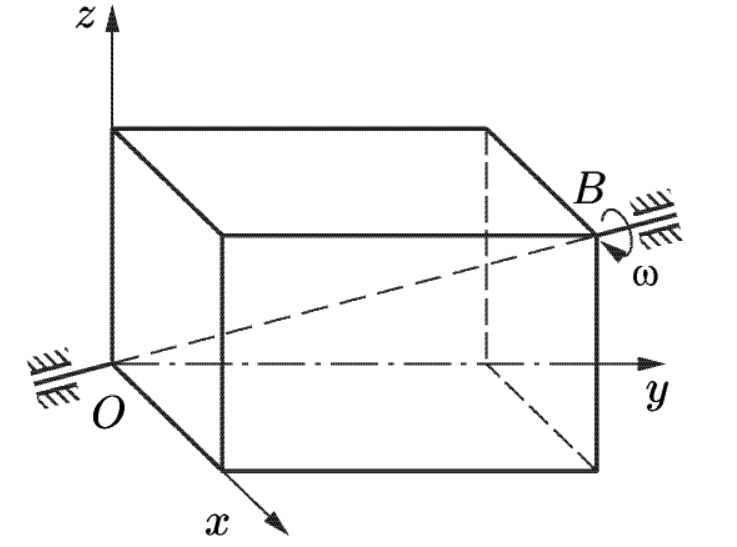
\includegraphics[width=0.99\textwidth]{figures/1.png}
            \caption{К задаче 11.18}
        \end{minipage}
        \hspace{0.5cm} 
        \begin{minipage}[b]{0.35\textwidth}
            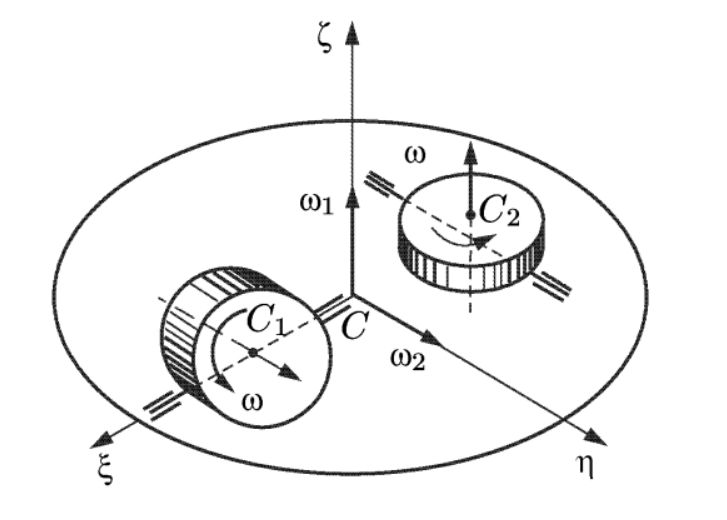
\includegraphics[width=0.9\textwidth]{figures/2.png}
            \caption{К задаче 11.27}
        \end{minipage}
        \hspace{0.5cm} 
        \begin{minipage}[b]{0.35\textwidth}
            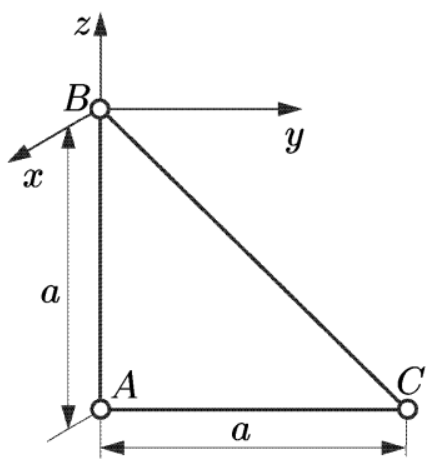
\includegraphics[width=0.65\textwidth]{figures/3.png}
            \caption{К задаче 11.27}
        \end{minipage}
    % \end{center}
\end{figure}


Поместим начало координат в центр масс (потому что так привычнее считать) и найдём тензор инерции по \eqref{t1} и \eqref{t2}, аналогично \eqref{t3}, несколько раз проинтегрировав по параллелепипеду 
\begin{align*}
    J_z = \rho \int_V (x^2 + y^2) \d V = \rho 
    \int\limits_{-a/2}^{a/2} \hspace{-2.5 mm} d x \hspace{-1.0 mm}
    \int\limits_{-b/2}^{b/2} \hspace{-2.5 mm} d y \hspace{-1.0 mm}
    \int\limits_{-c/2}^{c/2} \hspace{-2.5 mm} d z 
    \ (x^2 + y^2) = \frac{1}{12} m (a^2 + b^2),
\end{align*}
аналогичные результаты получим для $J_y, J_x$
\begin{equation*}
    J_y = \ \ldots \ = \frac{1}{12} m (a^2 + c^2),
    \hspace{1cm} 
    J_x = \ \ldots \ = \frac{1}{12} m (b^2 + c^2).
\end{equation*}
Остается найти осевые моменты инерции
\begin{equation*}
    J_{xy} = \rho \int_V x y \d V = \rho \frac{1}{16} a^2 b^2 c^2 = \frac{1}{16} m a b,
    \hspace{0.5cm} 
    J_yz = \ \ldots \ = \frac{1}{16} mbc,
    \hspace{0.5cm} 
    J_xz = \ \ldots \ = \frac{1}{16} mac.
\end{equation*}
Таким образом
\begin{equation}
    \hat{J}_O = \frac{1}{48} m 
    \begin{pmatrix}
        4(b^2+c^2) & -3ab & -3ac \\
        -3ab & 4(a^2+c^2) & -3bc \\
        -3ac & -3bc & 4(a^2+b^2) \\
    \end{pmatrix}.
\end{equation}
Кинетический момент найдём по определению, как
\begin{equation*}
    \mathbf{K}_O = \hat{J}_O \vc{\omega}, \hspace{0.5cm} 
    \mathbf{K}_A = \hat{J}_A \vc{\omega}, \hspace{0.5cm} 
\end{equation*}
где $\omega$ и $\hat{J}_A$ 
\begin{equation*}
    \hat{J}_A = \hat{J} + m \hat{j}_{OA},
    \hspace{1cm} 
    \vc{\omega} = \frac{\omega}{\sqrt{a^2+b^2+c^2}} 
    \left(a,\ b,\ c\right)\T
\end{equation*}
Заметим что $\hat{j}_{OA}$ будет аналогичен \eqref{t1}, тогда осталось найти $\mathbf{K}_O$:
\begin{equation*}
    \mathbf{K}_O = \hat{J}_O \vc{\omega}= \frac{\omega m}{48\sqrt{a^2+b^2+c^2}} 
    \begin{pmatrix}
        a (b^2+c^2) \\
        b (a^2 + c^2) \\
        c (a^2 + b^2) \\
    \end{pmatrix}.
\end{equation*}


%%%%%%%%%%%%%%%%%%%%%%%%%%%%%%%%%%%%%%%%%%%%%%%%%%%%%%%%%%%%%%%%%%%%%%%%%%%%%%%%%%%
\subsubsection*{11.27}

Проинтегрировав как в задачах 11.18 и 11.8(7) найдём, что относительно центра масс тензор инерции $\hat{J}_O$ диска в главных осях имеет вид
\begin{equation}
\label{t4}
    \hat{J}_C = \frac{1}{4} mR^2 \dmat{3}{1}{1}{2}.
\end{equation}
Кинетическая энергия тела может быть найдена, как
\begin{equation*}
    T = \frac{1}{2} \vc{\omega}\T \hat{J}_O \vc{\omega} + \frac{1}{2} m v_O^2.
\end{equation*}
Запишем $T$ для случая $\vc{\omega}_1 \parallel Oz$, как сумму вращательной и поступательной энергии для двух дисков. 

Поступательные, в силу геометрии системы, у дисков равны, первый диск вращается с угловой скоростью $\vc{\omega}_{\text{D1}}=(0,\ 0,\ \omega+\omega_1)$, а второй с $\vc{\omega}_{\text{D2}}=(0,\ \omega,\ \omega_1)$. Тензор инерции для второго диска аналогичен \eqref{t4}, только с 2 по оси $Oy$. Собирая всё вместе
\begin{equation*}
    T = 2 \times \frac{1}{2} m \omega_1^2 a^2 + 
    \underbrace{
        \frac{1}{4} mR^2 (\omega + \omega_1)^2
    }_{
    \vv{\omega}_{\text{D1}}\T \hat{J}_{0, \text{D1}} \vv{\omega}_{\text{D1}}
    }
     + 
     \underbrace{
     \frac{1}{8} mR^2 \omega_1^2 + \frac{1}{4} mR^2 \omega^2
     }_{
    \vv{\omega}_{\text{D2}}\T \hat{J}_{0, \text{D2}} \vv{\omega}_{\text{D2}}
     } =
     \frac{1}{2} m R^2 \omega^2 + \left(a^2 + \frac{3}{8} R^2\right) \omega_1^2 + \frac{1}{2} m R^2 \omega \omega_1.
\end{equation*}
Также заметим, что вопросы задачи симметричны с точностью до замены дисков, что упрощает нам дело в плане поиска и записи ответа:
\begin{equation}
    T_i = \frac{1}{2} m R^2 \omega^2 + \left(a^2 + \frac{3}{8} R^2\right) \omega_i^2 + \frac{1}{2} m R^2 \omega \omega_i,
    \hspace{1cm} i = 1, 2.
\end{equation}


%%%%%%%%%%%%%%%%%%%%%%%%%%%%%%%%%%%%%%%%%%%%%%%%%%%%%%%%%%%%%%%%%%%%%%%%%%%%%%%%%%%
\subsubsection*{11.92}
Найдём тензор инерции для точки $B$ по \eqref{t2}:
\begin{equation*}
    \hat{J}_B = ma^2 
    \begin{pmatrix}
        3 & 0 & 0 \\
        0 & 2 & 1 \\
        0 & 1 & 1 \\
    \end{pmatrix}.
\end{equation*}
Вспоминая результаты задачи №11.12, где подобное приведение к главным осям решено в общем виде, находим
\begin{equation*}
    B' = \frac{1}{2} \left(3+\sqrt{5}\right), \hspace{1cm}
    C' = \frac{1}{2} \left(3 - \sqrt{5} \right).
\end{equation*}
Главные оси же параллельны векторам
\begin{equation*}
    \vc{e}_1' = \left(1,\ 0,\ 0\right), \hspace{0.5cm} 
    \vc{e}_2' = \left(0,\ -2,\ \sqrt{5}-1\right), \hspace{0.5cm} 
    \vc{e}_3' = \left(0,\ 1-\sqrt{5},\ -2\right).
\end{equation*}
Отнормировав которые найдём новый базис.

Тензор инерции точки $A$ и эллипсоид инерции, соответственно, равны
\begin{equation*}
    \hat{J}_A = ma^2 \dmat{3}{2}{1}{1},
    \hspace{1cm} 
    M = \{2x^2 + y^2 + z^2 = 1\},
\end{equation*}
где $M$, как можно заметить, является эллипсоидом инерции ($J_y = J_z$). %done
\subsection{Динамика твёрдого тела}

\subsubsection*{11.45}
Твердое тело с неподвижной точкой движется под действием момента 
\begin{equation*}
    \vc{M}_O = \vc{a} \times \vc{\omega},
\end{equation*}
где вектор $\vc{a}$ вращается вместе с твёрдым телом.
Хотим перейти к динамическим уравнениям Эйлера, так что
\begin{equation*}
    \hat{J}_O = \dmat{3}{A}{B}{C}, \hspace{0.5cm} 
    \vc{\omega} = \begin{pmatrix}
        p \\ q \\ r
    \end{pmatrix},
    \hspace{0.5cm} 
    \vc{a} = \begin{pmatrix}
        a_\xi \\ a_\eta \\ a_\zeta
    \end{pmatrix}, 
    \hspace{0.5cm} 
    \vc{M}_O = \begin{pmatrix}
        a_\eta r - a_\zeta q \\
        a_\zeta p - a_\xi r \\
        a_\xi r - a_\eta p
    \end{pmatrix}.
\end{equation*}
Для начала попробуем в лоб, домножив динамические уравнения эйлера на $p, q, r$ соответсвенно
\begin{equation*}
    \left\{\begin{aligned}
        A \dot{p} + (C-B) q r &= - M_{\xi} \\
        B \dot{q} + (A-C) p r &= - M_{\eta} \\
        C \dot{r} + (B-A) p q &= - M_{\zeta} \\
    \end{aligned}\right.,
    \hspace{0.5cm} \Rightarrow \hspace{0.5cm}
    A \dot{p} p + B \dot{q} q + C \dot{r} r = 0.
\end{equation*}
Не густо. 

Пойдём в чуть более низкоуровневую запись
\begin{equation*}
    \frac{d \vc{K}_O}{d t} = \dot{K}_{Oi} \vc{e}_i + \vc{\omega} \times \vc{K}_O = \vc{a} \times \vc{\omega}.
\end{equation*}
Т.к. $\dot{a}_{i} \vc{e}_i = 0$, то
\vspace{-1mm}
\begin{equation*}
    (\dot{K}_{Oi} + \dot{a}_{i}) \vc{e}_i + \vc{\omega} \times (\vc{K}_O+\vc{a}) = 0
    \hspace{0.25cm} \Rightarrow \hspace{0.25cm} 
    \frac{d }{d t} \left(\vc{K}_O + \vc{a}\right) = 0
    \hspace{0.25cm} \Rightarrow \hspace{0.25cm} 
    \boxed{
       \vc{K}_O + \vc{a}   = \const
    } \text{ --- первый I интеграл}.
\end{equation*}
Теперь, т.к. $\vc{\omega} \bot \vc{M}_O$ предположим, что $T = \const$. Действительно
\begin{equation*}
    d T = \partial A = \cancel{\left(
        \vc{R} \cdot \vc{v}_O
    \right)} \d t +
    \cancel{\left(\vc{M})_O \cdot \vc{\omega}\right)} \d t = 0
    \hspace{0.5cm} \Rightarrow \hspace{0.5cm} 
    \boxed{
        T = \const
    }  \text{  -- второй I интеграл.}
\end{equation*}
\subsubsection*{11.59}

Есть твёрдое тело в отсутсвие внешних сил с $\vc{K}_O = \const$ и $A = B \neq C$. Выберем в качестве оси динамической симметрии ось $O\zeta$. Запишем динамические уравнения Эйлера
\begin{equation*}
    \left\{\begin{aligned}
        A \dot{p} + (C-A) qr &= 0 \\
        A \dot{q} - (C-A) pr &= 0 \\
        C \dot{r} &= 0
    \end{aligned}\right.
    \hspace{0.5cm} \Rightarrow \hspace{0.5cm} 
    C \dot{r} = 0, \hspace{0.5cm} Cr_0 = K_O \cos \theta = \const
    \hspace{0.5cm} \Rightarrow \hspace{0.5cm} 
    \left\{\begin{aligned}
        r(t) &= r_0 &= \const\\
        \theta(t) &= \theta &= \const
    \end{aligned}\right.
\end{equation*}
Посмотрим теперь на $\|\vc{K}_O\|$
\begin{equation*}
    K_O^2 = A^2 (p^2 + q^2) + (K_O \cos \theta)^2
    \hspace{0.5cm} \Rightarrow \hspace{0.5cm} 
    p^2 + q^2 = \left(\frac{K_0 \sin \theta}{A} \right)^2.
\end{equation*}
Теперь посмотрим на $\vc{\omega}$
\begin{equation*}
    \vc{\omega} = \dot{\vc{\varphi}} + \dot{\vc{\psi}} + \cancel{\dot{\vc{\theta}}},
\end{equation*}
проецируя всё на базис $O\xi\eta\zeta$ нахожим, что
\begin{equation*}
    \left\{\begin{aligned}
        r = \dot{\varphi} + \dot{\psi} \cos \theta \\
        \sqrt{p^2 + q^2} = \dot{\psi} \sin \theta       
    \end{aligned}\right.
    \hspace{0.5cm} \Rightarrow \hspace{0.5cm} 
   \left\{\begin{aligned}
       \dot{\psi} &= {K_O}/{A} &= \const \\
       \dot{\varphi} &= r_0 \left(1 - {C}/{A} \right) &=\const
   \end{aligned}\right.
\end{equation*}
Теперь мы готов записать \textit{параметры регулярной прецессии в случае Эйлера}:
\begin{equation}
\label{regp}
    \cos \theta = \frac{Cr_0}{K_0}, \hspace{0.5cm}
    \dot{\psi} = \frac{K_O}{A}, \hspace{0.5cm} 
    \dot{\varphi} = r_0 \left( 1- \frac{C}{A}  \right),
    \hspace{1cm} 
    K_O = \sqrt{C^2 r_0^2 + A^2 (\omega^2_0 - r_0^2)}.
\end{equation}

\subsubsection*{11.63}

Для начала поймём куда диск движется, точнее найдем (или хотя бы сделаем шаги в эту сторону) мгновенную ось вращения проходящую через точку $A$ и некоторую точку $C$.

Для начала посмотрим на геометрию системы (введя неизвестные $a, b, c$):
\begin{equation*}
    \vv{AB} = \begin{pmatrix}
        -r \\ -r \\ 0
    \end{pmatrix},
    \hspace{0.25cm} 
    \vv{AD} = \begin{pmatrix}
        r \\ -r \\ 0
    \end{pmatrix},
    \hspace{0.25cm} 
        \vv{CA} = \begin{pmatrix}
        a \\ b \\ c
    \end{pmatrix},
    \hspace{0.5cm} 
    \left\{\begin{aligned}
    \vc{v}_A &= \vc{\omega} \times \vv{CA} = 0\\
    \vc{v}_B &= \vc{\omega} \times \vv{CB} \\
    \vc{v}_A &= \vc{\omega} \times \vv{CD}
    \end{aligned}\right.,
    \hspace{0.5cm} 
    \left\{\begin{aligned}
        \vv{CD} &= \vv{CB} + \vv{BD} \\
        \vv{CD} &= \vv{CA} + \vv{AD} \\
        \vv{CB} &= \vv{CA} + \vv{AB}
    \end{aligned}\right.,
\end{equation*}
Для удобства далее будем считать $\vc{\omega} = {k} \vv{CA}$. Посчитаем векторы скоростей в нашеих обозначениях
\begin{equation*}
    \vc{v}_D = kr \begin{pmatrix}
        c \\ c \\ -b - a
    \end{pmatrix}
    \vc{v}_B = k \vv{CA} \times \vv{AB} = k r
    \begin{pmatrix}
        c \\ - c \\ b-a
    \end{pmatrix}
    \hspace{0.5cm} \Rightarrow \hspace{0.5cm} 
    a = b
\end{equation*}
Так как мы знаем абсолютные значения скоростей точек, то запишем
\begin{equation*}
    v_D^2 - v_B^2 = v_0^2 = 4 a^2 k^2
    \hspace{0.5cm} \Rightarrow \hspace{0.5cm} 
    a = \frac{v_0}{2rk}.
\end{equation*}
Подставив теперь значения $a$ в $v_B^2$ получим
\begin{equation*}
    v_B^2 = 2 k^2 c^2 r^2 = v_0^2
    \hspace{0.5cm} \Rightarrow \hspace{0.5cm} 
    c = \frac{v_0 \sqrt{2}}{2kr},
    \hspace{0.5cm} \Rightarrow \hspace{0.5cm} 
    \vc{\omega} = k \begin{pmatrix}
        a \\ b \\ c
    \end{pmatrix} = \frac{v_0}{2r} \begin{pmatrix}
        1 \\ 1 \\ \sqrt{2}
    \end{pmatrix}
\end{equation*}
Теперь найдём скорость центра масс
\begin{equation*}
    \vc{v}_O = \vc{\omega} \times \vc{r}_{CO} = 
    \vc{\omega} \times \left(
        \vc{r}_{CA} + \vv{AO}
    \right) = \vc{\omega} \times \begin{pmatrix}
        0 \\ - r \\ 0
    \end{pmatrix} = 
    \frac{v_0}{2} \begin{pmatrix}
        -\sqrt{2} \\ 0 \\ 1
    \end{pmatrix},
    \hspace{0.5cm} \Rightarrow \hspace{0.5cm} 
    \vc{r}_O(t) = 
    \begin{pmatrix}
        v_0 t / \sqrt{2} \\
        0 \\
        -gt^2/2+v_0 t / 2
    \end{pmatrix}.
\end{equation*}
Теперь мы знаем как будет двигаться в условиях гравитации наш диск (его центр масс)! 

Теперь посмотрим на вращение диска относительно центра масс. Для этого пересядем в СО падающую с $\vc{g}$, теперь $\vc{M}_O = \vc{0}$ и мы пришли к случаю Эйлера (который подробно был рассмотрен в задаче №11.59).

Для начала вспомним, что для диска кинетический момент
\begin{equation*}
    \vc{K}_O = \hat{J}_O \vc{\omega} = 
    \frac{m r^2}{4} \dmat{3}{1}{1}{2} 
    \begin{pmatrix}
        1 \\ 1  \\ \sqrt{2} 
    \end{pmatrix}
    \frac{v_0}{2r}  = \frac{mrv_0}{8} \begin{pmatrix}
        1 \\ 1 \\ 2 \sqrt{2}
    \end{pmatrix} = \const,
    \hspace{0.5cm} \Rightarrow \hspace{0.5cm} 
    K_O = \frac{\sqrt{10}}{8} mrv_0.
\end{equation*}
Зная $\vc{K}_O$ можем найти ось прецессии $\vc{e} \parallel \vc{K}_O$
\begin{equation*}
    \vc{e} = \frac{1}{\sqrt{10}} \left(1, \ 1, \ 2 \sqrt{2}\right).
\end{equation*}
Подставляя параметры системы в уравнения \eqref{regp}, найдём
\begin{equation*}
    \dot{\psi} = \frac{K_O}{A} = \frac{\sqrt{10}}{2} \frac{v_0}{r} ,
    \hspace{1cm} 
    \dot{\varphi} = r_0 \left(1 - \frac{C}{A} \right) =  
    -\frac{v_0 \sqrt{2}}{2r},
    \hspace{1cm} 
    \cos \theta = \frac{Cr_0}{K_O} = \frac{2\sqrt{5}}{5}.
\end{equation*}

\subsubsection*{11.72}

Решим чуть более общую задачу о движении тяжелого симметричного волчка с неподвижней нижней точкой. Начало координат $O$ совпадает с неподвижной точкой волчка, расстояние до центра масс равно $l$. 

Запишем кинематические и динамические уравнения Эйлера
\begin{equation*}
    \left\{\begin{aligned}
        p &= \dot{\varphi} \sin \theta \sin \psi + \dot{\theta} \cos \psi,\\
        q &= \dot{\varphi} \sin \theta \cos \psi - \dot{\theta} \sin \psi,\\
        r &= \dot{\varphi} \cos \theta + \dot{\psi}.
    \end{aligned}\right.,
    \hspace{0.6cm} 
    \left\{\begin{aligned}
        I_1 \dot{p} + (I_3-I_2) q r &= - M_{\xi} \\
        I_2 \dot{q} + (I_1-I_3) p r &= - M_{\eta} \\
        I_3 \dot{r} + (I_2-I_1) p q &= - M_{\zeta} \\
    \end{aligned}\right.,   
    \hspace{0.6cm} 
    \hat{J}_O = \dmat{3}{I_1}{I_1}{I_3}, \hspace{0.6cm} 
    \vc{\omega} = \begin{pmatrix}
        p \\ q \\ r
    \end{pmatrix}.
\end{equation*}
Кинетическая энергия волчка (с учетом параллельного переноса тензора инерции с центра масс к точке $O$)
\begin{equation*}
    T = \vc{\omega}\T \hat{J}_O \vc{\omega} = 
    \frac{I_1+ml^2}{2} \left(\dot{\theta}^2+\dot{\varphi}^2\sin^2 \theta\right) + \frac{1}{2} I_3 \left(\dot{\psi}+ \dot{\varphi} \cos \theta \right)^2.
\end{equation*}
Потенциальная энергия, соответсвенно, равна
\begin{equation*}
    \Pi = mgl \cos \theta.
\end{equation*}
Собирая вместе, находим
\begin{equation*}
    L = T - \Pi.
\end{equation*}
Понятно, что $K_3 = \const$, докажем также что $K_z = \const$. Действительно,
\begin{equation*}
    \frac{d K_z}{d t} = {\vc{M}_A}\bigg|_Z + \cancel{\vc{Q} \times \vc{v}_O} = 0
    \hspace{0.5cm} \Rightarrow \hspace{0.5cm} 
    K_z = \const.
\end{equation*}
Явно выпишем их
\begin{equation}
\label{ll1}
    \left\{\begin{aligned}
        K_3 &= {\partial L}/{\partial \dot{\psi}} = I_3\left(\dot{\psi} + \dot{\varphi} \cos \theta\right) \\
        K_z &= {\partial L}/{\partial \dot{\varphi}} = 
        \left((I_1+ml^2) \sin^2 \theta + I_3 \cos^2 \theta\right) \dot{\varphi} + I_3 \dot{\psi} \cos \theta.
    \end{aligned}\right.
\end{equation}
Кроме того, в системе сохраняется энергия
\begin{equation*}
    E = T + \Pi = \frac{1}{2} (I_1 + ml^2) \left(\dot{\theta}^2+\dot{\varphi}^2 \sin^2 \theta\right) 
    + \frac{1}{2} I_3 \left(\dot{\psi} + \dot{\varphi} \cos \theta\right)^2 + mgl\cos \theta.
\end{equation*}
Из \eqref{ll1} находим явные выражения для $\dot{\varphi}$ и $\dot{\theta}$ 
\begin{align*}
    \dot{\varphi} &= \frac{K_z - K_3 \cos \theta}{(I_1 + ml^2)\sin^2\theta} ,\\
    \dot{\psi} &= \frac{K_3}{I_3}  - \cos \theta \frac{K_z - K_3 \cos \theta}{(I+ml^2)\sin^2 \theta} .
\end{align*}
Подставляя это в выражения для энергии $E$ получим
\begin{equation}
    E  = \frac{1}{2} (I_1 + ml^2) \dot{\theta}^2 +
    \frac{
        (K_z - K_3 \cos \theta)^2
    }{
        2 (I_1 + ml^2) \sin^2 \theta
    } + \frac{K_3^2}{2I_3} + mgl \cos \theta.
\end{equation}
Таким образом мы находим 
\begin{equation}
    \dot{\theta} = \frac{d \theta}{d t} = f_{\dot{\theta}}(E, K_z, K_3)
    \hspace{0.5cm} \Rightarrow \hspace{0.5cm} 
    t = \int_{\theta_0}^\theta \frac{d \theta}{f_{\dot{\theta}}(E, K_z, K_3)},
\end{equation}
что и является нашим искомым решением в квадратурах. Конкретно для №11.72 следует положить $I_3=0$ и, в силу доступного для стержня произволя, $\dot{\psi}=0$. Слагаемые вида $K_3/I_3$ в таком случае просто не возникнут, решение сохранится.
















\subsubsection*{11.118}

Как и в решение к №11.72 у нас симметричный волчок. Требуется определить начальную угловую скорость прецессии $\dot{\varphi}_0$, чтобы $\dot{\theta}=0$. 
Формально можем поставить задачу несколько иначе, какой должен быть момент внешних сил $\vc{M}_O$ чтобы происходила регулярная прецессия $\dot{\theta}=0$?

Для начала введём отдельно $\vc{\omega}_1 \parallel O\xi$ и $\vc{\omega}_2 \parallel OZ$.
 По раннее проделанной работе с регулярной прецессией, мы знаем, что $K_z$ и $K_3$ постоянны, соответсвенно $\omega_1, \omega_2, \omega = \const$.
 Аналогично случаю Эйлера (см. №???)
 \begin{equation*}
     (K_O)_\xi = Cr, \hspace{0.5cm} (K_O)_Z = A \sqrt{q^2 + q^2}.
 \end{equation*}
 То есть $\vc{K}_O \in O\xi Z$ и $K_O=\const$. Но, т.к. плоскость $O\xi Z$ вращаеся с угловой скорсотью $\vc{\omega}_2$ то и вектор $\vc{K}_O$ аналогично. Тогда для $\vc{M}_O$ верно, что
 \begin{equation}
     \frac{d \vc{K}_O}{d t} = \vc{\omega}_2 \times \vc{K}_O = \vc{M}_O.
 \end{equation}
 Нетрудно показать, что
 \begin{equation*}
     \vc{\omega}_2 \times \vc{K}_O = 
     \frac{\vc{\omega}_2\times \vc{\omega}_1}{\|\vc{\omega}_2\times \vc{\omega}_1\|} \omega_2 \sin \theta
     \left(
        C (\omega_1 + \omega_2 \cos \theta) - A \omega_2 \cos \theta
     \right) 
 \end{equation*}
 Т.к. $\|\omega_2 \times \omega_1\| = \omega_1 \omega_2 \sin \theta$, то
 \begin{equation}
 \label{ggg}
    \vc{M}_O = 
     (\vc{\omega}_2 \times \vc{\omega}_1) \left[
        C + (C-A) \frac{\omega_2}{\omega_1} \cos \theta
     \right].
 \end{equation}
 Это \textit{основная формула гироскопии}, так что, наверное, можно было принять её на веру. В частном случае, когда $\omega_1 \gg \omega_2$ можно приближенно записать эту формулу, как
 \begin{equation}
     \vc{M}_O = C \left(\vc{\omega}_2 \times \vc{\omega}_1\right).
 \end{equation}

 Конкретно для нашей задачи \eqref{ggg} перепишется как
 \begin{equation*}
     \dot{\varphi} \omega \sin \theta 
     \left(
        C + (C-A) \frac{\dot{\varphi}}{\omega} \cos \theta
     \right) = mgl \sin \theta,
 \end{equation*}
 т.к. мы действительно требуем регулярной прецессии. Так получаем квадратное уравнение вида
 \begin{equation}
     (C-A) \dot{\varphi}^2 \cos \theta + C \omega \varphi - mgl = 0
     \hspace{0.5cm} \Rightarrow \hspace{0.5cm} 
     \dot{\varphi} = 
     \frac{
        - C \omega \pm \sqrt{
            C^2 \omega^2 + (C-A) mgl \cos \theta
        }
     }{
        2(C-A) \cos \theta
     }  .
 \end{equation}
Стоит заметить, что при $C^2 \omega^2 + (C-A) mgl \cos \theta < 0$ регулярная прецессия, по всей видимости, невозможна. При $\omega >> \dot{\varphi}$ угловая прецессия будет равна
\begin{equation}
    \dot{\varphi} = \frac{mgl}{C\omega},
\end{equation}
и, как видно, не зависит от угла нутации. 

Теперь про силы. Запишем II закон Ньтона в проекции на вертикаль и нормаль к вертикали, повернутую на $+\varphi$ от $X$, получим
\begin{equation}
    \left\{\begin{aligned}
        N_x = m \dot{\varphi}^2 l \sin \theta \\
        N_y - mg = 0        
    \end{aligned}\right.
    \hspace{0.5cm} \Rightarrow \hspace{0.5cm} 
    N = m\sqrt{g^2 + \dot{\varphi}^2 l^2 \sin^2 \theta}.
\end{equation}
\subsubsection*{Т.16*}


Запишем динамические уравнения Эйлера
\begin{equation}
    \left\{\begin{aligned}
        A \dot{p} + (C-B) q r &= - M_{\xi} \\
        B \dot{q} + (A-C) p r &= - M_{\eta} \\
        C \dot{r} + (B-A) p q &= - M_{\zeta} \\
    \end{aligned}\right.,
    \hspace{1cm} 
    \vc{\omega} = \begin{pmatrix}
        p \\ q \\ r
    \end{pmatrix}, 
    \hspace{1cm} 
    \hat{J}_O = \dmat{3}{A}{B}{C}.
\end{equation}
Тело вращается относительно закрепленного центра масс $O$. По условию
\begin{equation*}
    \vc{M}_O = - \gamma \vc{\omega},
    \hspace{1cm} 
    A = B > C.
\end{equation*}
Хочется доказать, что мгновенная ось вращения тела асимптотически стремится стать ортогональной оси динамической симметрии тела ($O\zeta$). Если чуть формализовать, то 
\begin{equation}
\label{lim}
    \lim_{t \to \infty} \frac{\|\vc{\omega}^{\zeta}\|}{\|\vc{\omega}^{\xi\eta}\|} = \frac{r}{\sqrt{p^2+q^2}} = 0,
\end{equation}
равносильно поставленному условию.

Конкретизируем динамические уравнения Эйлера под наш случай:
\begin{align}
        A \dot{p} + (C-A) qr &= -\gamma p \label{eq1} \\
        A \dot{q} - (C-A) pr &= -\gamma q \label{eq2} \\
        C \dot{r} &= -\gamma r \label{eq3}
\end{align}
Из \eqref{eq3} найдём
\begin{equation*}
    r = \omega^{\zeta} = r_0 \exp \left(-\frac{\gamma}{C} t\right).
\end{equation*}
Теперь посмотрим на $p \cdot \eqref{eq1} + q \cdot \eqref{eq2}$ равное полному дифференциалу по времени
\begin{equation*}
    p \dot{p} + q \dot{q} = 
    \frac{1}{2} \frac{d }{d t} \left(p^2 + q^2 \vp \right)
    =
    - \frac{\gamma}{A} \left(\vp p^2 + q^2 \right).
\end{equation*}
Естественно решить это уравнение относительно $\omega^{\xi\eta}$
\begin{equation*}
    \omega^{\xi\eta} = - \frac{\gamma}{A} \omega^{\xi\eta}
    \hspace{0.5cm} \Rightarrow \hspace{0.5cm} 
    \sqrt{p^2+q^2} = \omega^{\xi\eta} = \omega^{\xi\eta}_0 
    \exp \left(-\frac{\gamma}{A} t\right).
\end{equation*}
Подставляя всё в \eqref{lim} находим
\begin{equation*}
    \lim_{t \to \infty} \ 
    \left[\frac{\omega^{\zeta}}{\omega^{\xi\eta}}\right] =
    \frac{r_0}{\omega^{\xi\eta}_0} \cdot
    \lim_{t \to \infty} 
\bigg[    \exp \bigg(
        \frac{\gamma}{AC} \underbrace{(C-A)\vp}_{<0} t
    \bigg) \bigg] = 0, 
    \hspace{1cm} 
    \text{Q. E. D.}
\end{equation*}


 %done

\section{Аналитическая механика}
\setcounter{subsection}{9}
\subsection{Уравнения Лагранжа}

\begin{figure}
\begin{minipage}[t]{0.3\textwidth}
    \centering
    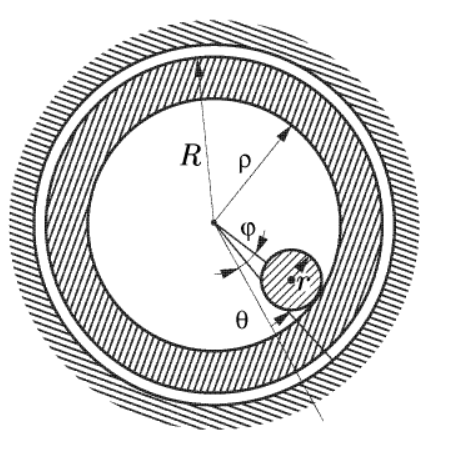
\includegraphics[width=0.9\textwidth]{figures/12.46.png}
    \caption{К задаче 12.46}
    \label{t12n46}
\end{minipage}
\hfill
\begin{minipage}[t]{0.3\textwidth}
    \centering
    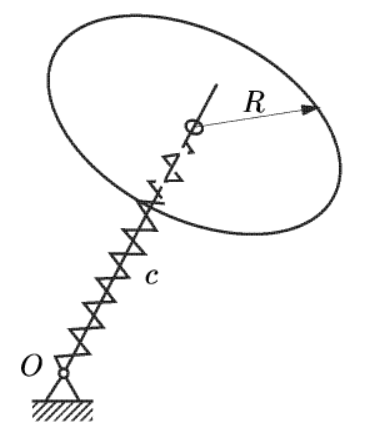
\includegraphics[width=0.8\textwidth]{figures/12.59.png}
    \caption{К задаче 12.59}
    \label{t12n59}
\end{minipage}
\hfill
\begin{minipage}[t]{0.3\textwidth}
    \centering
    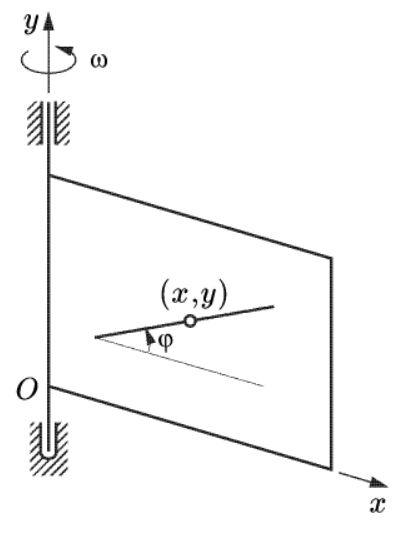
\includegraphics[width=0.8\textwidth]{figures/12.61.png}
    \caption{К задаче 12.61}
    \label{t12n61}
\end{minipage}
\end{figure}



\subsubsection*{12.6 (в)}

Проверим, является ли интегрируемой связь 
\begin{equation*}
    \dot{y} - z \dot{x} = 0.
\end{equation*}
В случае интегрируемости связи существовали бы запрещенные положения системы. Покажем же что в действительности мы можем попасть из любой точки в любую. В силу отсутсвия ограничений на $\dot{z}$, мы свободно можем перемещаться вдоль оси $z$ при $\dot{x}, \dot{y} = 0$. Пусть мы оказались в $z = 2$, тогда при движении
\begin{equation*}
    \letus \ \dot{x} \d t = \xi,
    \ \ \dot{y} \d t=  2 \xi, \hspace{0.5cm} \Rightarrow \hspace{0.5cm} 
    (0, 0, 2) \longrightarrow (\xi, 2 \xi, 2).
\end{equation*}
Теперь по $\dot{x}, \dot{y} = 0$ перейдём в $z = 1$, тогда
\begin{equation*}
    \letus \ \dot{x} \d t = -\xi, \ \ \dot{y} \d t = -\xi,
    \hspace{0.5cm} \Rightarrow \hspace{0.5cm} 
    (\xi, 2 \xi, 1) \longrightarrow (0, \xi, 1).
\end{equation*}
Собирая всё вместе,
\begin{equation*}
    (0, 0, 0)
    \overset{\vv{\dot{r}} = (0, 0, \neq 0)}{\longrightarrow} 
    (0, 0, 2)
    \overset{\vv{\dot{r}}dt = (\xi, 2\xi, 2)}{\longrightarrow} 
    (\xi, 2 \xi, 2)
    \overset{\vv{\dot{r}} = (0, 0, \neq 0)}{\longrightarrow} 
    (0, 0, 1)
    \overset{\vv{\dot{r}}dt = (-\xi, -\xi, 1)}{\longrightarrow} 
    (0, \xi, 1)
    \overset{\vv{\dot{r}} = (0, 0, \neq 0)}{\longrightarrow} 
    (0, \xi, 0).
\end{equation*}
Получается допустимы перемещения из $\vc{r}_1$ в $\vc{r}_2$ $\forall \vc{r}_1, \vc{r}_2$, следовательно \textbf{связь не является интегрируемой}.


\subsubsection*{12.12}

Найдём уравнения движения для двух материальных точек, массами $m_1$ и $m_2$, притягивающихся по закону Ньютона. В качестве обобщенных координат выберем $x, y, z$ центра масс системы, расстояние между точками $r$ и углы $\varphi, \theta$, определяющие направление прямой. 

Потенциальная энергия системы $\Pi$ 
\begin{equation*}
    \Pi = - \gamma \frac{m_1 m_2}{r}.
\end{equation*}
Для каждого из тел можем записать расстояние до центра масс и абсолютное положение:
\begin{equation*}
    r_1 = \frac{m_2}{m_1+m_2} r, \hspace{0.5cm} 
    r_2 = \frac{m_1}{m_1+m_2} r,
    \hspace{0.5cm} 
    \left\{\begin{aligned}
        x_1 &= x + r_1 \sin \theta \cos \varphi, \\
        y_1 &= y + r_1 \sin \theta \cos \varphi, \\
        z_1 &= z + r_1 \cos \theta.
    \end{aligned}\right.
    \hspace{0.5cm} 
    \left\{\begin{aligned}
        x_2 &= x + r_2 \sin \theta \cos \varphi, \\
        y_2 &= y + r_2 \sin \theta \cos \varphi, \\
        z_2 &= z + r_2 \cos \theta.
    \end{aligned}\right.
\end{equation*}
Вспомнив, что для сферических координат$(r,  \theta, \varphi)$ метрический тензор $g_{ij} = \diag \left({1}, \ {r^2}, \ {r^2 \sin^2 \theta} \right)$, найдём  квадрат относительной скорости
\begin{equation*}
    v_1^2(r_1) = g_{ij} \dot{q}^i \dot{q}^j = 
    r_1^2 \sin^2 \theta \dot{\varphi}^2 + r_1^2 \dot{\theta}^2 + \dot{r_1}^2 
    \hspace{0.5cm} \Rightarrow \hspace{0.5cm} 
    v_1^2(r_1) = \left(
    \frac{m_2}{m_1+m_2} 
    \right)^2 \cdot v_1^2 (r).
\end{equation*}
Теперь можем записать кинетическую энергию движения ($T_1, T_2$ -- кинетические энергии движения тел относительно центра масс) :
\begin{equation*}
    T_1 + T_2 + \frac{1}{2} (m_1+m_2) \left(\frac{d}{dt} (x, \ y, \ z)\right)^2 =
    \frac{1}{2} \frac{m_1 m_2}{m_1 + m_2} 
    \left(
        r^2 \sin^2 \theta \dot{\varphi}^2 + r^2 \dot{\theta}^2 + \dot{r}^2
    \right) + 
    \frac{1}{2} (m_1+m_2) \left(\dot{x}^2 + \dot{y}^2 + \dot{z}^2\right).
\end{equation*}
И, наконец, лагранжиан системы
\begin{equation}
    L = T - \Pi = \frac{1}{2} \frac{m_1 m_2}{m_1 + m_2} 
    \left(
        r^2 \sin^2 \theta \dot{\varphi}^2 + r^2 \dot{\theta}^2 + \dot{r}^2
    \right) + 
    \frac{1}{2} (m_1+m_2) \left(\dot{x}^2 + \dot{y}^2 + \dot{z}^2\right)
    + \gamma \frac{m_1 m_2}{r}.
\end{equation}
Найдём уравнения движения системы относительно центра масс:
\begin{equation}
    \left\{\begin{aligned}
        \frac{d }{d t} \frac{\partial L}{\partial \dot{\varphi}} - \frac{\partial L}{\partial \varphi} &= 0 \\
        \frac{d }{d t} \frac{\partial L}{\partial \dot{r}} - \frac{\partial L}{\partial r} &= 0 \\
        \frac{d }{d t} \frac{\partial L}{\partial \dot{\theta}} - \frac{\partial L}{\partial \theta} &= 0.
    \end{aligned}\right.
    \hspace{0.5cm} \Rightarrow \hspace{0.5cm} 
    \left\{\begin{aligned}
        \dot{\varphi} \left(
        r  \dot{\theta} \sin (2 \theta) + \dot{r} \dot{\varphi} (1 - \cos 2 \theta)
    \right) 
    + \frac{1}{2} r \ddot{\varphi} \left(
         1 - \cos 2 \theta
    \right) = 0, 
    \\
        \gamma (m_1 + m_2) - r^3
    \left(
        \sin^2 \theta \dot{\varphi}^2 + \dot{\theta}^2
    \right) + r^2 \ddot{r} = 0,
    \\
    2 \dot{\theta} \dot{r} + r \ddot{\theta} - \frac{1}{2} r \sin (2 \theta) \dot{\varphi}^2 = 0.
    \end{aligned}\right.
\end{equation}
И для центра масс:
\begin{equation}
    \ddot{x} = 0, \hspace{0.5cm} 
    \ddot{y} = 0, \hspace{0.5cm} 
    \ddot{z} = 0.
\end{equation}
Что логично, на центр масс не действует никаких сил.

Теперь к интегралам системы. Пусть $\frac{d }{d t} (x_1, y_1, z_1)\T = \vc{v}_1$, аналогично для второго тела. Во-первых сохраняется количество движения системы
($x, \ y, \ z$ не входят явно в $L$), также не входят $t, \ \varphi$, тогда
\begin{equation}
    \left\{\begin{aligned}
        \frac{d }{d t} \frac{\partial L}{\partial x} &= 0 \\
        \frac{d }{d t} \frac{\partial L}{\partial \varphi} &= 0 \\
        L &\neq L(t)
    \end{aligned}\right.    
    \hspace{0.5cm} \Rightarrow \hspace{0.5cm} 
    \left\{\begin{aligned}
        m_1 \vc{v}_1 + m_2 \vc{v}_2 &= \const, \\
        r^2 \dot{\varphi} \sin^2 \theta  &= \const, \\
        E = \Pi + T &= \const.
    \end{aligned}\right.
\end{equation}
Вообще, в силу отсутсвия внешних сил на систему, сохраняется кинетический момент,
\begin{equation}
    \vc{K} = m_1 \vc{r}_1 \times \vc{v}_1 + 
    m_2 \vc{r}_2 \times \vc{v}_2 = \const.
\end{equation}

\subsubsection*{12.29}

Два однородных стержня длины $l$ каждый образую плоский двойной маятник. Составим уравнения движения в форме Лагранжа. 

Выберем начала координат в точке подвеса. Тогда координаты центра масс второго стержня
\begin{equation*}
    \left\{\begin{aligned}
        x_2 &= l \sin \varphi_1 + (l/2) \sin \varphi_2, \\
        y_2 &= l \cos \varphi_1 + (l/2) \cos \varphi_2.
    \end{aligned}\right.
\end{equation*}
Потенциальная энергия системы
\begin{equation*}
    \Pi = -mg \left(\frac{l}{2} \cos \varphi_1 \right) -
    mg \left(
        l \cos \varphi_1 + \frac{l}{2} \cos \varphi_2
    \right).
\end{equation*}
Кинетическая энергия первого стержня
\begin{equation*}
    T_1 = \frac{1}{2} I_1 \dot{\varphi}_1^2 = \frac{l^2 m}{6}  \dot{\varphi}^2.
\end{equation*}
Для второго стержня найдём кинетическую энергию, рассмотрев его вращение относительно центра масс:
\begin{equation*}
    T_2 = \frac{1}{2} m \left( \dot{x}_2^2 + \dot{y}_2^2\right) +
    \frac{1}{2} \frac{m l^2}{12}  \dot{\varphi}_2^2.
\end{equation*}
Лагранжиан системы:
\begin{equation}
    L = T - \Pi 
    =  ml^2 \left[
        \frac{g}{2l} \left( 3 \sin \varphi_1 +  \cos \varphi_2  \right)
        + \frac{1}{2} \cos (\varphi_1 - \varphi_2) \dot{\varphi}_1 \dot{\varphi}_2 + \frac{2}{3}  \dot{\varphi}^2 + \frac{1}{6} \dot{\varphi}_2^2
        \right].
\end{equation}
Тогда уравнения движения системы
\begin{equation}
    \left\{\begin{aligned}
        \frac{d }{d t} \frac{\partial L}{\partial \dot{\varphi_1}} - \frac{\partial L}{\partial \varphi_1} &= 0, \\
        \frac{d }{d t} \frac{\partial L}{\partial \dot{\varphi_2}} - \frac{\partial L}{\partial \varphi_2} &= 0.
    \end{aligned}\right.
    \hspace{0.5cm} \Rightarrow \hspace{0.5cm} 
    \left\{\begin{aligned}
    9 (g/l) \sin \varphi_1 + 3  \sin (\varphi_1 - \varphi_2) \dot{\varphi}^2_2
    + 3 \cos (\varphi_1 - \varphi_2) \ddot{\varphi}_2 + 8  \ddot{\varphi}_1 &= 0, \\
    3 (g/l) \sin \varphi_2 - 3  \sin (\varphi_1 - \varphi_2) \dot{\varphi}_1^2
    + 3 \cos (\varphi_1 - \varphi_2) \ddot{\varphi}_1 + 2  \ddot{\varphi}_2 &= 0.
    \end{aligned}\right.
\end{equation}
\subsubsection*{12.46}

Составим уравнения движения в форме Лагранжа для системы, представленно на рис. \ref{t12n46} Для начала запишем потенциальную энергию системы, как
\begin{equation*}
    \Pi = - (\rho - r) \cos (\varphi  + \theta).
\end{equation*}
Момент инерции полого цилиндра:
\begin{equation*}
    I_1 = \int_\rho^R \sigma r^2 \d V 
    \hspace{0.2cm} 
    \overset{dV = h 2 \pi r \d r}{\longrightarrow} 
    \hspace{0.2cm} 
    I_1 = 2 \pi \sigma h \int_\rho^R r^3 \d r = 
    \frac{1}{2} \left(R^2 - \rho^2  \right) (R^2 + \rho^2) \pi  h \sigma =
    \frac{1}{2} M \left(R^2 + \rho^2\right).
\end{equation*}
Тогда его кинетическая энергия 
\begin{equation*}
    T_1 = \frac{1}{4} M \left(R^2 + \rho^2\right) \dot{\theta}^2.
\end{equation*}
Скорость центра масс сплошного цилиндра:
\begin{equation*}
    v_2 = \dot{\varphi} (\rho  - r).
\end{equation*}
Пусть цилиндр катится с угловой скоростью $\omega$, тогда запишем условие того, что он не проскальзывает
\begin{equation*}
    (\rho - r) \dot{\varphi} = \rho \dot{\theta} + \omega r,
    \hspace{0.5cm} \Rightarrow \hspace{0.5cm} 
    \omega = (\rho - r) \dot{\varphi} - \rho \dot{\theta}.
\end{equation*}
Тогда кинетическая энергия сплошного цилиндра
\begin{equation*}
    T_2 = 
    \frac{1}{2} m \left(
        \dot{\varphi} (\rho - r) \vp
    \right)^2 + 
    \frac{1}{2} \left(\frac{1}{2} m r^2 \right) \omega^2
    .
\end{equation*}
Лагранжиан системы:
\begin{equation}
    L = 
    mg (\rho - r) \cos \varphi +
     m \left(
        \frac{1}{2}  \dot{\varphi}^2 (\rho - r)^2 + 
        \frac{1}{4} \left(
            \dot{\theta} \rho - \dot{\varphi} (\rho - r)
        \right)^2
    \right) + \frac{1}{4} M \left(R^2  + \rho^2\right)\dot{\theta}^2.
\end{equation}
Соответсвенно, уравнения движения системы
\begin{equation}
    \left\{\begin{aligned}
        \frac{d }{d t} \frac{\partial L}{\partial \dot{\varphi}} - \frac{\partial L}{\partial \varphi} &= 0, \\
        \frac{d }{d t} \frac{\partial L}{\partial \dot{\theta}} - \frac{\partial L}{\partial \theta} &= 0.
    \end{aligned}\right.
    \hspace{0.5cm} \Rightarrow \hspace{0.5cm} 
    \left\{\begin{aligned}
    - \ddot{\theta} \rho + 3 \ddot{\varphi} \left(\rho - r\right) + 2 g \sin{\left(\varphi \right)} &= 0, \\
    M \ddot{\theta} \left(R^{2} + \rho^{2}\right) + \rho m \left(\ddot{\theta} \rho - \ddot{\varphi} \left(\rho - r\right)\right) &= 0.
    \end{aligned}\right.
\end{equation}
\subsubsection*{12.59}

Составим уравнения движения в форме Лагранжа для системы, представленнйо на рис. \ref{t12n59}. Для начала перейдём в сферические координаты:
\begin{equation*}
    \left\{\begin{aligned}
        x &= r \sin \theta \cos \varphi, \\
        y &= r \sin \theta \cos \varphi, \\
        z &= r \cos \theta.
    \end{aligned}\right.
\end{equation*}

Для начала запишем потенциальную энергию системы, как
\begin{equation*}
    \Pi = mg z + \frac{1}{2} k (r_0 - r)^2.
\end{equation*}
Как уже было показано в №12.12 скорость центра масс диска
\begin{equation*}
     v^2 = g_{ij} \dot{q}^i \dot{q}^j = 
    r^2 \sin^2 \theta \dot{\varphi}^2 + r^2 \dot{\theta}^2 + \dot{r}^2.
\end{equation*}
Также запишем кинематические уравнения Эйлера и момент инерции диска:
\begin{equation*}
    \vc{\omega} \overset{\text{в СО диска}}{=}  \begin{pmatrix}
        \omega_1 \\
        \omega_2 \\
        \omega_3 
    \end{pmatrix},
    \hspace{1cm} 
    \left\{\begin{aligned}
        \omega_1 &= \dot{\psi} \sin \theta \sin \varphi + \dot{\theta} \cos \varphi, \\
        \omega_2 &= \dot{\psi} \sin \theta \cos \varphi - \dot{\theta} \sin \varphi, \\
        \omega_3 &= \dot{\psi} \cos \theta + \dot{\varphi},
    \end{aligned}\right.
    ,
    \hspace{1cm} 
    \hat{J} = \frac{m R^2}{4} \dmat{3}{1}{1}{2}.
\end{equation*}
Кинетическую энергию диска тогда найдём, как
\begin{equation*}
    T = \frac{1}{2} \vc{\omega}\T \hat{J} \vc{\omega} + \frac{1}{2} m 
    \left(r^2 \sin^2 \theta \dot{\varphi}^2 + r^2 \dot{\theta}^2 + \dot{r}^2\right).
\end{equation*}
Соответственно, лагранжиан системы:
% \begin{equation}
%     L = \frac{M \dot{\theta}^{2} \left(R^{2} + \rho^{2}\right)}{4} + \frac{\dot{\varphi}^{2} m \left(\rho - r\right)^{2}}{2} + g m \left(\rho - r\right) \cos{\left(\varphi \right)} + \frac{m \left(\dot{\theta} \rho - \dot{\varphi} \left(\rho - r\right)\right)^{2}}{4}.
% \end{equation}
\begin{equation}
    \begin{aligned}
        L/m =
            &+\frac{1}{8} R^{2} \left(\dot{\psi}^{2} \cos^{2} \theta + \dot{\psi}^{2} + 4 \dot{\psi} \dot{\varphi} \cos \theta + \dot{\theta}^{2} + 2 \dot{\varphi}^{2}\right) + \\
            &+ \frac{1}{2} r^2 \left(\dot{\theta}^{2} r^{2} + \dot{\varphi}^{2} r^{2} \sin^{2} \theta + \dot{r}^{2}\right)
            - \\
            &-  g r \cos \theta - \frac{1}{2} \frac{k}{m}  \left(r_{0} - r\right)^{2}.
    \end{aligned}
\end{equation}
Уравнения движения системы:
\begin{equation}
        \EqL{\varphi},\hspace{0.5cm} 
        \EqL{\theta}, \hspace{0.5cm} 
        \EqL{\psi}, \hspace{0.5cm} 
        \EqL{r}. 
\end{equation}
Подставляя $L$, получим уравнения движения в чуть менее элегантной форме:
\begin{equation}
    \begin{aligned}
        R^{2} \left(\ddot{\psi} \cos{\left(\theta \right)} + \ddot{\varphi} - \dot{\psi} \dot{\theta} \sin{\left(\theta \right)}\right) + 2 \ddot{\varphi} r^{2} \sin^{2}{\left(\theta \right)} + 2 \dot{\theta} \dot{\varphi} r^{2} \sin{\left(2 \theta \right)} + 4 \dot{\varphi} \dot{r} r \sin^{2}{\left(\theta \right)} &= 0, \\
        %%%%%%%%%%%%%%%%%%%%%%%%%%%%%%%%%%%%%%%%%%%%%%%%%%%%%%%%%%%%%%%%%%%%%%%%%%%%%%%%%%%
        R^{2} \ddot{\theta} + R^{2} \dot{\psi} \left(\dot{\psi} \cos{\left(\theta \right)} + 2 \dot{\varphi}\right) \sin{\left(\theta \right)} + 4 \ddot{\theta} r^{2} + 8 \dot{\theta} \dot{r} r - 2 \dot{\varphi}^{2} r^{2} \sin{\left(2 \theta \right)} - 4 g r \sin{\left(\theta \right)} &= 0, \\
        %%%%%%%%%%%%%%%%%%%%%%%%%%%%%%%%%%%%%%%%%%%%%%%%%%%%%%%%%%%%%%%%%%%%%%%%%%%%%%%%%%%
        \ddot{\psi} \cos^{2}{\left(\theta \right)} + \ddot{\psi} + 2 \ddot{\varphi} \cos{\left(\theta \right)} - \dot{\psi} \dot{\theta} \sin{\left(2 \theta \right)} - 2 \dot{\theta} \dot{\varphi} \sin{\left(\theta \right)} &= 0, \\
        %%%%%%%%%%%%%%%%%%%%%%%%%%%%%%%%%%%%%%%%%%%%%%%%%%%%%%%%%%%%%%%%%%%%%%%%%%%%%%%%%%%
        2 \ddot{r} m + 2 g m \cos{\left(\theta \right)} - 2 k \left(- r + r_{0}\right) - 2 m r \left(\dot{\theta}^{2} + \dot{\varphi}^{2} \sin^{2}{\left(\theta \right)}\right) &= 0.
    \end{aligned}
\end{equation}
\subsubsection*{12.61}

Составим уравнения движения в форме Лагранжа для системы, представленно на рис. \ref{t12n61}. Хотелось бы найти уравнения относительного движения стержня в форме Лагранжа.

Потенциальная энергия стержня
\begin{equation*}
    \Pi = mgy.
\end{equation*}
Записав кинетическую энергию,, рассматривая движение центра масс и вращение относительно него, найдём 
\begin{equation}
    L = T - \Pi = 
    \frac{1}{2} m \left(
        \dot{y}^2 + \omega^2 x^2 + \dot{x}^2
    \right) + 
    \frac{1}{12} m l^2 \left(
        \dot{\varphi}^2 + \omega^2 \cos^2 \varphi
    \right) - mgy.
\end{equation}
В угловой скорости появляется добавка $\omega \cos \varphi$ как проекции $\vc{\omega}$ на нормаль к стержню. 

Уравнения движения системы найдём, как
\begin{equation}
    \left\{\begin{aligned}
        \EqL{x},  \\
        \EqL{y}, \\
        \EqL{\varphi}.
    \end{aligned}\right.
    \hspace{0.5cm} \Rightarrow \hspace{0.5cm} 
    \left\{\begin{aligned}
       \vp  \ddot{x} &= \omega^2 x,\\
       \vp  \ddot{y} &= g, \\
       \vp  \ddot{\varphi} &= -  \omega^2 \sin (2 \varphi) / 2.
    \end{aligned}\right.
\end{equation}
\subsubsection*{12.88}

Пусть на диск действует сила реакции опоры $\vc{N}_1$, на опору со стороны диска действует $\vc{N}_2 = - \vc{N}_1$ .  Связь по опрделению является идеальной, если
\begin{equation*}
    \delta A = \sum_i \left(
        \vc{N}_i \cdot \delta \vc{r}_i
    \right) = 0.
\end{equation*}
В рассматриваемой системе в проекцию на ось $Oy$  $\delta r_1 = \delta r_2$. Тогда
\begin{equation*}
    OY: \hspace{0.5cm} 
    \delta A = N_1 \delta r_1 + N_2 \delta r_2 = (N_1 - N_1) \delta r_1 = 0,
\end{equation*}
следовательно \textbf{связь является идеальной}.
\subsubsection*{12.73}
Выберем начало координат в положение равновесия. Запишем второй закон Ньютона для системы:
\begin{equation*}
    m \ddot{x} = -cx-\beta v.
\end{equation*}
Формально, мы хотим найти такой $L(x, \dot{x}, t)$, что 
\begin{equation*}
    \frac{d }{d t} \frac{\partial L}{\partial \dot{q}} - \frac{\partial L}{\partial q}  = m \ddot{x} + \beta \dot{x}  + cx = 0.
\end{equation*}
При отсутствии вязкого трения $L$ имел бы вид
\begin{equation*}
    L^* = T - \Pi = \frac{1}{2} m \dot{x}^2 + \frac{1}{2} cx^2.
\end{equation*}
Как мы видим $L^* \neq L(t)$, соответсвенно энергия такой системы сохраняется. Мы же рассматриваем систему с вязким трением, которая в пределе с $\beta \to 0$ приходила бы к $L = L^*$ так что будем искать $L$ вида 
\begin{equation*}
    L = f(t) \cdot L^*.
\end{equation*}
В таком случае
\begin{equation*}
    \frac{d }{d t} \frac{\partial L}{\partial \dot{q}} - \frac{\partial L}{\partial q}  =    
    f(t) m \ddot{x} + \underbrace{\dot{f} (t) m}_{= f(t) \beta}
     \dot{x}  + f(t) cx = 0
     \hspace{0.5cm} \Leftrightarrow \hspace{0.5cm} 
     m \ddot{x} + \beta \dot{x} +   c x = 0.
\end{equation*}
Воплощая в жизнь стремление сократить уравнение на $f(t)$ находим, что
\begin{equation*}
    \frac{d }{d t} f(t) = \frac{\beta}{m} f(t),
    \hspace{0.5cm} \Rightarrow \hspace{0.5cm} 
    f(t) = \exp\left(\frac{\beta}{m} t\right).
\end{equation*}
Тогда уравнене движения осциллятора с вязким трением можно записать, как уравнение лагранжа второго рода, для лагранжаиана
\begin{equation}
    L(x, t) = \exp \left(\frac{\beta}{m} t\right) \cdot \frac{1}{2} 
    \left(
        m \dot{x}^2 + c x^2
    \right).
\end{equation}
\subsubsection*{12.82}
Знаем, что символ Кристофеля
\begin{equation*}
    \Gamma_{i,kl} = \frac{1}{2} \left(
        \frac{\partial g_{li}}{\partial q^k} + \frac{\partial g_{ki}}{\partial q^l} -
        \frac{\partial g_{kl}}{\partial q^i} 
    \right).
\end{equation*}
Кинетическая энергия склерономной системы в обобщенных координатах запишется как
\begin{equation*}
    T  = \frac{1}{2} g_{ij} \dot{q}^i \dot{q}^j.
\end{equation*}
Хотелось бы в терминах сивола Кристофеля записать уравнения Лагранжа
\begin{equation*}
    \frac{d }{d t} \frac{\partial T}{\partial \dot{q}^i} - \frac{\partial T}{\partial q^i} = Q_i.
\end{equation*}

Для начала найдём
\begin{equation*}
    \frac{\partial T}{\partial q^k} = \frac{1}{2} \dot{q}^i \dot{q}^j \frac{\partial g_{ij}}{\partial q^k}.
\end{equation*}
Теперь
\begin{equation*}
    \frac{\partial T}{\partial \dot{q}^k} = 
    \frac{1}{2} g_{ij} \left(
        \dot{q}^j \delta^i_k + q\delta^i \delta^j_k
    \right) = g_{kj} \dot{q}^j.
\end{equation*}
Дифференцируя по времени, получим
\begin{equation*}
    \frac{d }{d t} \frac{\partial T}{\partial \dot{q}^k} =
    g_{kj} \ddot{q}^j + 
    \dot{q}^j \left(
        \frac{\partial g_{kj}}{\partial q^i} \frac{d q^i}{d t} 
    \right) = 
    g_{kj} \ddot{q}^j + \frac{\partial g_{kj}}{\partial q^i} \dot{q}^j \dot{q}^i.
\end{equation*}
Теперь заметим, что
\begin{equation*}
    \dot{q}^i \dot{q}^j \frac{\partial g_{kj}}{\partial q^i} =
     \dot{q}^j \dot{q}^i \frac{\partial g_{ki}}{\partial q^j} .
\end{equation*}
Тогда
\begin{equation}
    Q_k =
    g_{kj} \ddot{q}^j + \frac{1}{2} \dot{q}^j \dot{q}^i
    \left(
        \frac{\partial g_{jk}}{\partial q^i} + \frac{\partial g_{ik}}{\partial q^j} 
        - \frac{\partial g_{ij}}{\partial q^k} 
    \right) , \hspace{0.5cm} \Rightarrow \hspace{0.5cm} 
    \boxed{
        g_{kj} \ddot{q}^j + \Gamma_{k, ij} \dot{q}^j \dot{q}^i = Q_k
    }.
\end{equation} %done
\subsection{Принцип Гамильтона-Остроградского}


\subsubsection*{21.7}

Запишем лагранжиан системы
\begin{equation*}
    L = T - \Pi = \frac{1}{2} m \dot{x}^2 + \frac{1}{2} m x^2 \omega^2.
\end{equation*}
В условиях сказано, что $\omega = \omega(t)$ -- для простоты рассмотрим $\omega = \const$.

\begin{figure}[h]
    \centering
    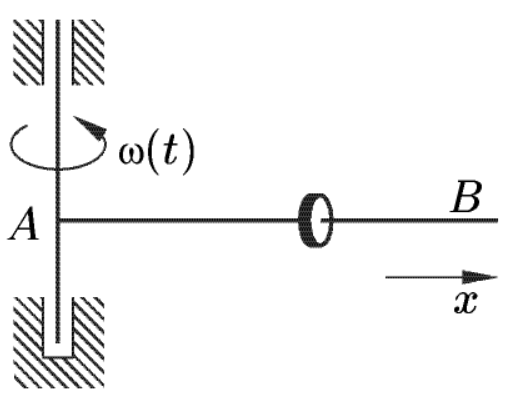
\includegraphics[width=0.25\textwidth]{figures/21.7.png}
    \caption{К задаче 21.7}
    %\label{fig:}
\end{figure}

Действие тогда
\begin{equation*}
    S = \int_{t_1}^{t_2} L \d t,
    \hspace{0.5cm} \Rightarrow \hspace{0.5cm} 
    \delta S = m
        \dot{x} \delta x \bigg|_{t_1}^{t_2}
        +
        m\int_0^t
        \left(
        - \ddot{x} + x \omega^2
        \right) \delta x \d t
     = 0.
\end{equation*}
Так приходим к
\begin{equation*}
    \ddot{x} = \omega^2 (t) x,
    \hspace{0.5cm} \Rightarrow \hspace{0.5cm} 
    x = A e^{\omega t} + B e^{-\omega t}.
\end{equation*}
Рассмотрим движение от $(x_1, t_1)$ до $(x_2, t_2)$, получим СЛУ:
\begin{equation*}
    \left\{\begin{aligned}
        x_1 &= A e^{\omega t_1} + B e^{-\omega t_1} \\
        x_2 &= A e^{\omega t_2} + B e^{-\omega t_2}
    \end{aligned}\right.
    \hspace{0.5cm} \Rightarrow \hspace{0.5cm} 
    \det = e^{\omega(t_1 - t_2)} - e^{-\omega(t_1 - t_2)} \neq 0,
     \hspace{0.25cm} \text{ при } t \neq \const,
\end{equation*}
что соответствует существованию единственного решения у уравнения.

Возвращаясь к случаю $\omega = \omega(t)$, хотелось бы показать, что решение задачи Коши
\begin{equation*}
    \left\{\begin{aligned}
        \dot{x}(x) &= \xi(t),\\
        \dot{\xi}(t) &= x(t) \omega^2 (t),
    \end{aligned}\right.
    \hspace{0.5cm} \text{c начальными условиями}
    \hspace{0.5cm} 
    \left\{\begin{aligned}
        x(t_1)   &= x_1, \\
        \xi(t_1) &= \xi_1,
    \end{aligned}\right.
\end{equation*}
существует и единственно. 

Действительно, из физических соображений, функция $\omega(t)$ непрерывна, соотвественно и $\xi(t), x(t)$, тогда решение задачи Коши существует и единственно для любых $t_1, t_2$. 
Для сравнения в Т17 $\varphi(t)$ не является непрерывной функцией, соответсвенно наблюдаем неединтсвенность решения. 

Решаем мы здесь правда краевые задачи, а не задачи Коши, поэтому общий случай нуждается ещё в дополнительном рассуждении. Скорее всего единственность решения будет определяться формой самого Лагранжиана.
\subsubsection*{21.14 и 21.15}

Точка массы $m$ може двигаться по гладкой вертикальной плоскости $xz$, вращающейчя вокруг векртикальной оси $Oz$ с постоянной угловой скоростью $\omega$. 

Лагранжиан системы
\begin{equation}
    L = \frac{1}{2} m \left(
        \dot{x}^2 + \dot{z}^2
    \right) + 
    \frac{1}{2} m x^2 \omega^2
    - mgz.
\end{equation}
Вариация действия
\begin{equation*}
    \delta S = m \int_{A}^{B} \left(
        \dot{x} \delta x + \dot{z} \delta z + \omega^2 x \delta x - g \delta z
    \right) \d t.
\end{equation*}
Посмотрим на действие
\begin{align*}
    S 
    &= \int_{A}^{B} 
    L(x+\delta x, z + \delta z, t) \d t = \\
    &= \int_{A}^{B}
    L(x, z, t) \d t + 
    \underbrace{
    m \int_{A}^{B} \dot{x} \delta \dot{x} + \dot{z} \delta \dot{z} + \omega^2 x \delta x - g \delta z \d t
    }_{\delta S (L(x, z, t)) = 0} +
    \frac{1}{2} m \int_{A}^{B}
     (\delta \dot{x})^2 + \left(\delta \dot{z}\right)^2 + \omega^2
     (\delta x)^2 \d t, \hspace{0.5cm} \text{Q.E.D.}
\end{align*}

\subsubsection*{21.35}

Хотелось бы от действия $S$ вида
\begin{equation*}
    S = \int_A^B L \d t, \hspace{0.5cm} 
    L = T - \Pi = \frac{1}{2} p_i \dot{q}^i - \Pi
\end{equation*}
к действию (или \textit{укороченному действию}) $\delta S^* = 0$, где $S^*$ вида
\begin{equation}
\label{sample}
    S^* = \int_A^B n \d s, \hspace{0.5cm} 
    \phantom{
    L = T - \Pi = \frac{1}{2} p_i \dot{q}^i - \Pi
    }
\end{equation}
где под интегрирование от $A$ до $B$ подразумевается интегрирование интегрирование уравнение от состояния в точке $A$ до состояния в точке $B$. Можно было бы сразу получить ответ из принципа Мопертюи, так что давайте его выведем. 

Перейдём к энергии системы, как функции $p$ и $q$, где $p_i = \partial L / \partial \dot{q}^i$ -- обобщенный импульс. Тогда
\begin{equation}
\label{I2135}
    dS = L \d t = \left(p_i  \dot{q}^i - H\right) \d t
    \hspace{0.5cm} \Rightarrow \hspace{0.5cm} 
    S  = S_0 - H \cdot(t_B-t_A), 
\end{equation}
так как мы рассматриваем аналогию с консервативной системой, то есть $\dot{H} = 0$. Величина $S_0$ -- \textit{укороченное действие},
\begin{equation*}
    S_0 = \int_A^B p_i \dot{q}^i \d t = 
    2 \int_A^B (H - \Pi) \d t.
\end{equation*}
Найдём $dt$, как
\begin{equation*}
    dt = \frac{ds}{v},
    \hspace{0.25cm} 
    v^2 = 2 (H-\Pi) / m
    \hspace{0.5cm} \Rightarrow \hspace{0.5cm} 
    dt = \frac{ds}{
    \sqrt{2(H-\Pi) / m}}.
\end{equation*}
Собирая всё вместе, получаем
\begin{equation*}
    S_0 = \int_A^B\sqrt{2m(H-\Pi)} \d s.
\end{equation*}
Вернёмся к варьированию. Если допускать варьирование конечного момента времени, то
\begin{equation}
\label{II2135}
    \delta S = \frac{\partial S}{\partial t}  \delta t = -H \delta t, \hspace{0.5cm} \Rightarrow \hspace{0.5cm} 
    \delta S + H \delta t = 0.
\end{equation}
Подставляя \eqref{I2135} в \eqref{II2135}, получим, что
\begin{equation}
    \delta S_0 = 0, 
    \hspace{0.5cm} \Rightarrow \hspace{0.5cm} 
    \delta \left(
        \int_A^B\sqrt{2m(H-\Pi)} \d s
    \right) = 0.
\end{equation}
Сравнивая полученное выражение с \eqref{sample}, полагая $m =1$, находим
\begin{equation}
    \Pi = -\frac{n^2}{2} + H.
\end{equation}


\subsubsection*{Т17.}

Рассмотрим движение точки по цилиндру радиуса $r_0$. Тогда $L$ 
\begin{equation*}
    L  = T - \Pi = T = \frac{1}{2} m v^2 = \frac{1}{2} m \dot{q}_i \dot{q}^i
    = \frac{1}{2} m g_{ij} \dot{q}^i \dot{q}^j
    = \frac{1}{2} \left(r_0^2 \dot{\varphi}^2 + \dot{z}^2\right)
    .
\end{equation*}
Тогда вариация действия для системы (свободной материальной точки)
\begin{equation*}
    \frac{d }{d t} (\dot{x} \delta x) = \ddot{x} \delta x + \dot{x} \delta \dot{x}
    \hspace{0.25cm} \Rightarrow \hspace{0.25cm} 
    \delta S =
    m \int_A^B 
    \left( 
        r_0^2 \dot{\varphi} \delta \dot{\varphi} + \dot{z} \delta \dot{z}
     \right)
    \d t = 
    m (r_0^2 \dot{\varphi} \delta \varphi + \dot{z} \delta z)\bigg|_A^B
    + 
    \int_A^B 
    \left(
        -r_0^2 \ddot{\varphi} \delta \varphi - \ddot{z} \delta z
    \right) \d t = 0.
\end{equation*}
Вариация на $A$ и $B$ тождественно равна 0, в силу прозвольности $\delta z$ и $\delta \varphi$ получаем, что
\begin{equation*}
    \left\{\begin{aligned}
        \ddot{\varphi} &= 0, \\
        \ddot{z} &= 0
    \end{aligned}\right.
    \hspace{0.5cm} \Rightarrow \hspace{0.5cm} 
    \left\{\begin{aligned}
        \varphi &= C_1 t + C_2 \mod 2 \pi, \\
        z &= C_3 t + C_4.
    \end{aligned}\right.
\end{equation*}
так как в силу выбора $\varphi$ верно, что $\varphi + 2 \pi k = \varphi \ \  \forall k \in \mathbb{Z}$. В таком случае
\begin{equation*}
    C_1 = \frac{\varphi_B - \varphi_A}{t_B - t_A} + \frac{2\pi}{t_B - t_A} k,
    \hspace{0.5cm} \forall k \in \mathbb{Z},
\end{equation*}
таким образом для свободной материальной точки существует счётное количество истинных путей для перемещения из $A$ в $B$ за фиксированное время $t_B - t_A$.

\subsubsection*{Задача о траектории луча (оптический принципа Ферма $\sim$ принципа Мопертеи-Лагранжа)}

Найдём траекторию светового луча в среде с показателем преломления
\begin{equation*}
    n(z) = n_0 + n_z z.
\end{equation*}
Согласно принципу Ферма, введя $(ds)^2 = (dr)^2 + (dz)^2$, считая $dz / dr = \dot{z}$
\begin{equation*}
    \delta \left(
        \int_A^B (n_0 + n_z z) \d s
    \right) = 0,
\hspace{0.5cm} \Rightarrow \hspace{0.5cm} 
    \delta
    \left(
        \int_A^B z \sqrt{1 + \dot{z}^2} \d r
    + \frac{n_0}{n_z}  l 
    \right) = 0,
\end{equation*}
где
\begin{equation*}
    l = \int_A^B \sqrt{1 + \dot{z}^2} \d r.
\end{equation*}
Вспомнив \eqref{lstar} и \eqref{intl}, 
поймём, что решаем изопериметрическую задачу, которую уже решили в предыдущем пункте, решением является траектория по цепной линии, с $\lambda = -n_0/n_z$:
\begin{equation}
    z(r) = \frac{n_0}{n_z} + C_1 \ch \frac{r-C_2}{C_1},
\end{equation}
где $C_1$ и $C_2$ определяются из начальных условий\footnote{
    Предполагая, что мы хотим пустить луч от точки $(z_1, r_1)$ к $(z_2, r_2)$, мы сможем сделать это единственным образом, это и задаст $C_1$ и $C_2$.
}.



\subsubsection*{Задача о цепной линии}

Решим задачу о цепной линии. Пусть в точках $(x_1, y_1)$ и $(x_2, y_2)$ закреплена цепь с линейной плотностью $\rho$ и массой $M$.
Для цепной линии сначала найдём центр масс $y_0$:
\begin{equation*}
    y_0 = \frac{1}{M} \int_{x_1}^{x_2}
    y \cdot 
    \underbrace{
    \rho \sqrt{1 + (y_x')^2} \d x
    }_{
    dm
    }.
\end{equation*}
Лагранжиан системы
\begin{equation*}
    L = T - \Pi = M g \cdot y_0.
\end{equation*}
В силу независимости $L$ от $t$ верно, что
\begin{equation}
    \delta S = \delta 
    \left(\int_{t_1}^{t_2} L \d t\right)
    = 0,
    \hspace{0.5cm} \Rightarrow \hspace{0.5cm} 
    \delta L = 0, \hspace{0.5cm} \Rightarrow \hspace{0.5cm}
    \delta
    \bigg(
    \int_{x_1}^{x_2}
    \underbrace{
    y \sqrt{1 + (y_x')^2}
    }_{
    F(x)
    } \d x
    \bigg) = 0
    ,
\end{equation}
что позволяет нам решать немного другую задачу.

Мы знаем, что на $\dot{q}, q$ равносильны следующие условия
\begin{equation*}
    \frac{d }{d t} \frac{\partial L(\dot{q}, q, t)}{\partial q^i}  - \frac{\partial L}{\partial q}  = 0,
    \hspace{0.5cm} \Leftrightarrow \hspace{0.5cm} 
    \delta \left(
        \int_{t_1}^{t_2} L(\dot{q}, q, t) \d t
    \right) = 0,
\end{equation*}
при фиксированной длине нити $l$ равной
\begin{equation}
\label{intl}
    l = \int_{x_1}^{x_2} \underbrace{
    \sqrt{1+\dot{y}^2}
    }_{\varphi(x)} \d x,
\end{equation}
где $y_x' = \dot{y}$ (здесь и далее). 
Тогда введём\footnote{
    О причинах такого решения см. метод решения изопериметрической задачи.
} $L^*$
\begin{equation}
\label{lstar}
    L^* (y, x) = F(x) - \lambda \varphi(x),
\end{equation}
для которого верно, что
\begin{equation}
\label{maeq}
\delta \left(\int_{x_1}^{x_2} L^*(y, \dot{y}, x) \d x \right) = 0
\hspace{0.5cm} \Leftrightarrow \hspace{0.5cm} 
    \frac{d}{dx} \frac{\partial L^*}{\partial \dot{y}} -\frac{\partial L^*}{\partial x} = 0.
\end{equation}
Формально мы перещли к решению изопериметрической задачи. Для удобство переобозначим $L^* = L$. 
Посмотрим на $\partial L / \partial \dot{y} = L_{\dot{y}}$:
\begin{equation*}
    d L_{\dot{y}} (y, \dot{y}) = 
    \frac{\partial L_{\dot{y}}}{\partial y} \d y + 
    \frac{\partial L_{\dot{y}}}{\partial \dot{y}} \d \dot{y},
    \hspace{0.5cm} \Rightarrow \hspace{0.5cm} 
    \frac{d }{d x} \frac{\partial L}{\partial \dot{y}} -\frac{\partial L}{\partial y} =
    L_{\dot{y}, y} \dot{y} + L_{\dot{y}, \dot{y}} \ddot{y} - L_{y} = 0.
\end{equation*}
Домножив на $(-\dot{y})$ получим, как видно, полный дифференциал \rotatebox[origin=c]{270}{:)}
\begin{equation*}
    \frac{\partial L}{\partial y} \frac{d y}{d x} 
    + \underbrace{
    \frac{\partial L}{\partial \dot{y}} \frac{d \dot{y}}{d x} 
    - \bigg(
        \frac{\partial L}{\partial \dot{y}} \ddot{y}
    }_{\text{прибавил/вычел}}
     + 
        \dot{y} \bigg[
            \frac{\partial L_{\dot{y}}}{\partial y} \dot{y} + \frac{\partial L_{\dot{y}}}{\partial \dot{y}} \ddot{y}
        \bigg]
    \bigg)
    = \frac{d }{d x} \left(
        L - \dot{y} \frac{\partial L}{\partial \dot{y}} 
    \right),
\end{equation*}
откуда \eqref{maeq} может быть переписано, как
\begin{equation*}
    L - \dot{y} \frac{\partial L}{\partial \dot{y}} = C_1,
\end{equation*}
то есть да, <<энергия>> сохраняется, $x$ же явно не входит в $L^*$. 

Конкретно в нашем случае,
\begin{equation*}
    (y+\lambda) \sqrt{1 + \dot{y}^2}
    - \dot{y} (y + \lambda) \frac{\dot{y}}{\sqrt{1+\dot{y}^2}}  = C_1,
    \hspace{0.5cm} \Rightarrow \hspace{0.5cm} 
    y + \lambda = C_1 \sqrt{1 + \dot{y}^2}.
\end{equation*}
Как известно 
\href{https://ru.wikipedia.org/wiki/%D0%A8%D0%B8%D0%BD%D1%83%D1%81}{шинус} замечателен: $1 + \sh^2 \varkappa = \ch^2 \varkappa$, так что пусть $\dot{y} = \sh \varkappa$. Тогда
\begin{equation*}
    y = C_1 \ch \varkappa - \lambda.
\end{equation*}
Подставив друг в друга последних два выражения, найдём
\begin{equation*}
    \dot{y} = \frac{d y}{d \varkappa} \cdot \frac{d \varkappa}{d x} 
    = C_1 \frac{d \varkappa}{d x} 
    \sh \varkappa,
    \hspace{0.5cm} \Rightarrow \hspace{0.5cm} 
    x  = C_1 \varkappa + C_2.
\end{equation*}
Таким образом мы получаем \textit{уравнение цепной линиии}
\begin{equation}
    \boxed{
        y = C_1 \ch \frac{x-C_2}{C_1} - \lambda.
    }
\end{equation}
Константы могут быть найдены из граничных условий $y(x_1)=y_1$, $y(x_2)=y_2$
и интеграла \eqref{intl}:
\begin{equation*}
     \sh \frac{x_2 - C_2}{C_1} - \sh \frac{x_1 - C_2}{C_1} = \frac{l}{C_1}.
\end{equation*} 


\subsubsection*{Т19.}

\red{Пока не готово.} %done -T19!
\subsection{Равновесие. Принцип виртуальных перемещений.}

% 14.37, 14.20, 14.34, 14.41

\subsubsection*{14.37}

Перейдём в СО, вращающуюся с $\vc{\omega}$, соотвественно хочется ввести потенциальное поле для сил инерции и гравитационных.
\begin{align*}
    \d F_{\text{ц. б.}} &= \omega^2 x \d m, 
    \hspace{0.5cm} \Rightarrow \hspace{0.5cm} 
    \d \Pi_{\text{и}} = - \frac{1}{2} \omega^2 x^2 \d m.
\end{align*}
Тогда потенциал
\begin{align*}
    \Pi_{\text{g}, 1} &= - \frac{m}{l} \int_0^{l \sin \varphi}
    \frac{1}{2} \omega^2 x^2 \d x  = 
    - \frac{m_1 l^2}{6} \omega^2 \sin^2 \varphi. \\
    \Pi_{\text{g}, 2} &= - \frac{m_2 l^2}{6} \omega^2 \sin^2 \varphi.
\end{align*}
Полная энергия системы:
\begin{equation*}
    \Pi = -gl \cos \varphi \left(m_1 + \frac{3}{2} m_2\right) - \frac{1}{6} \omega^2 l^2 \sin^2 \varphi (m_1 + m_2).
\end{equation*}
Найдём стационарные точки потенциала
\begin{equation*}
    \frac{\partial E}{\partial \varphi} = \frac{1}{2} gl \sin \varphi  (m_1 + 3 m_2)
    - \frac{1}{3} \omega^2 l^2 \sin \varphi \cos \varphi (m_1 + m_2) = 0.
\end{equation*}
Находим положения равновесия:
\begin{equation*}
    \sin \varphi^* = 0, \hspace{0.5cm} \Rightarrow \hspace{0.5cm} \varphi^* = 0, \ \pi.
\end{equation*}
При условии, что rhs следующего уравнения $\leq 1$, найдём также
\begin{equation*}
    \cos \varphi^* = \frac{2g (m_1 + 3 m_2)}{2 \omega^2 (m_1 + m_2)},
    \hspace{0.5cm} 
    \omega^2 \geq \frac{3g (m_1 + 3m_2)}{2l(m_1+m_2)}.
\end{equation*}


\subsubsection*{14.20}

Перейдём в СО точки подвеса. В таком случае можно ввести потенциальное поле, гравитационного поля
\begin{equation*}
    \vc{g}' = \vc{g} - \vc{w}.
\end{equation*}
Положение равновесия соответсвует минимуму потенциала, соответственно наименьший $h_{\text{ц. м.}}$ относительно $\vc{g}'$. В таком случае при $\vc{w} \parallel \vc{g}$ ниточка останется висеть вертикально. При $\vc{g} \nparallel \vc{w}$, вводя начало координат в точку подвеса
\begin{equation}
    y = x \frac{g - w \sin \alpha}{w \cos \alpha}, \hspace{0.5cm} 
    a \neq \frac{\pi}{2} + \pi k.
\end{equation}



\subsubsection*{14.34}


Система движется в потениальном поле с удерживающией связью:
\begin{equation*}
    \Pi = \sum_{k=1}^n \alpha_k q_k, \hspace{1cm} 
    \sum_{k=1}^n\alpha_k^2 > 0, \hspace{1cm} 
    \sum_{k=1}^n q_k^2 - 1 \leq 0.
\end{equation*}
Можно было решить задачу на условный экстремум, введя функцию $F$:
\begin{equation*}
    f = \sum_{k=1}^n \alpha_k q_k - \lambda \left(
        \sum_{k=1}^n q_k^2 - 1
    \right).
\end{equation*}
А моожно посмотреть на $n$-мерную сферу, которой ограничено положение системы на координатном пространстве. Действующая сила тогда
\begin{equation*}
    \frac{\partial \Pi}{\partial q^i} = F_i = \alpha_i,
    \hspace{0.5cm} \Rightarrow \hspace{0.5cm} 
    \vc{F} = \left(\alpha_1, \ \ldots,\  \alpha_n\right)\T.
\end{equation*}
Уравнение для сферы
\begin{equation*}
    \sum q_i^2 = 1.
\end{equation*}
Нас интересует момент, когда радиус вектор сонаправлен с $\vc{F}$, пусть $\vc{r} = k \vc{F}$.
\begin{equation*}
    (k \alpha_1)^2 + \ldots + (k \alpha_n)^2 = 1,
    \hspace{0.5cm} \Rightarrow \hspace{0.5cm} 
    k = \left(
        \sum_{k=1}^n \alpha_k^2
    \right)^{-1/2}.
\end{equation*}
Соответсвенно искомое положение равновесия
\begin{equation}
    \vc{r} = \left(
        \sum_{k=1}^n \alpha_k^2
    \right)^{-1/2} \left(\alpha_1,\  \ldots, \ \alpha_n\right)\T.
\end{equation}
\subsubsection*{14.41}

Материальная точка может двигаться по линии пересечения двух плоскостей:
\begin{equation*}
    \left\{\begin{aligned}
        &\text{I}: &-2x_1 + x_2 + x_3  &= t \\
        &\text{II}: &x1 - 2x_2 + x_3 &= -t^2.
    \end{aligned}\right.
\end{equation*}
Найдём систему бесконечно малых возможных перемещений.
Знаем, что направляющая прямой,
\begin{equation*}
    \vc{n}_\text{I} \times \vc{n}_\text{II} = 
    \begin{pmatrix}
        -2 \\ 1 \\ 1
    \end{pmatrix} \times
    \begin{pmatrix}
        1 \\ -2 \\ 1
    \end{pmatrix} = 3 \begin{pmatrix}
        1 \\ 1 \\ 1
    \end{pmatrix},
    \hspace{0.5cm} \Rightarrow \hspace{0.5cm} 
    \vc{a} = \begin{pmatrix}
        1 \\ 1 \\ 1
    \end{pmatrix}.
\end{equation*}
Хотелось бы найти уравнения прямой, в виде
\begin{equation*}
    \vc{r} = \vc{r}_0 + \vc{a} k.
\end{equation*}
Подставляя $\vc{a}$ в уравнения плоскости, найдём, что
\begin{equation*}
    x_0 = \frac{1}{3} t (t-2), \hspace{0.5cm} 
    y_0 = \frac{1}{3} t (2t - 1), \hspace{0.5cm} 
    z_0 = 0.
\end{equation*}
Тогда
\begin{equation*}
    \vc{r} = \frac{t}{3} \begin{pmatrix}
        t - 2 \\ 2t -1 \\ 0
    \end{pmatrix} + 
    k \begin{pmatrix}
        1 \\ 1 \\ 1
    \end{pmatrix},
    \hspace{0.5cm} \Rightarrow \hspace{0.5cm} 
    \frac{\partial \vc{r}}{\partial t} =
    \frac{1}{3} \begin{pmatrix}
        2t-2 \\ 4t-1 \\ 0
    \end{pmatrix},
    \hspace{0.5cm} 
    \frac{\partial \vc{r}}{\partial k} = \begin{pmatrix}
        1 \\ 1 \\ 1
    \end{pmatrix}.
\end{equation*}
В таком случае возможные перемещения:
\begin{equation*}
    \delta \vc{r} = \begin{pmatrix}
        1 \\ 1 \\ 1
    \end{pmatrix} \delta k,
    \hspace{1cm} 
    d \vc{r} = \delta \vc{r} + \frac{\partial \vc{r}}{\partial t} \d t = 
    \begin{pmatrix}
        1 \\ 1 \\ 1
    \end{pmatrix} \delta k + 
    \frac{1}{3} \begin{pmatrix}
        2t-2 \\ 4t-1 \\ 0
    \end{pmatrix} dt.
\end{equation*}














 %done
\subsection{Устойчивость равновесия консервативных систем.}

% 15.5, 15.9, 15.13, 15.23*

\begin{figure}
\begin{minipage}[t]{0.36\textwidth}
    \centering
    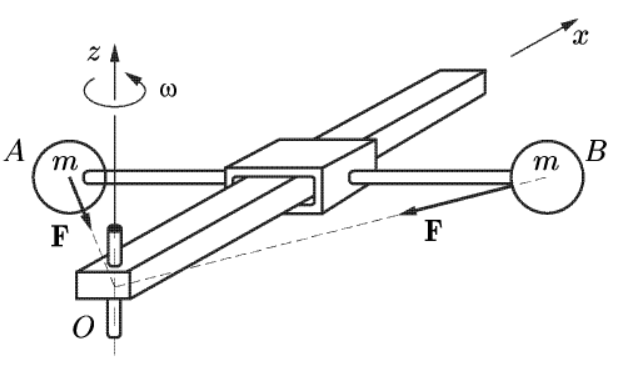
\includegraphics[width=0.9\textwidth]{figures/15_5.png}
    \caption{К задаче 15.5}
\end{minipage}
\hfill
\begin{minipage}[t]{0.36\textwidth}
    \centering
    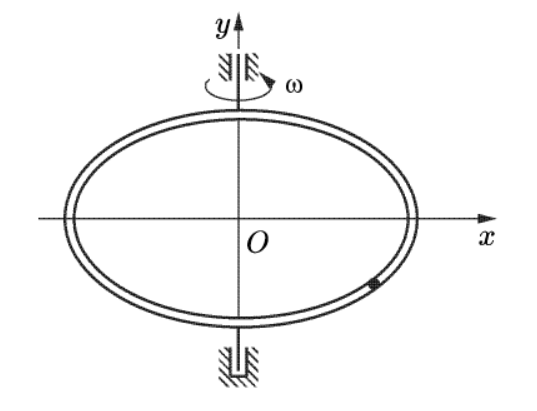
\includegraphics[width=0.9\textwidth]{figures/15_9.png}
    \caption{К задаче 15.9}
\end{minipage}
\hfill
\begin{minipage}[t]{0.2\textwidth}
    \centering
    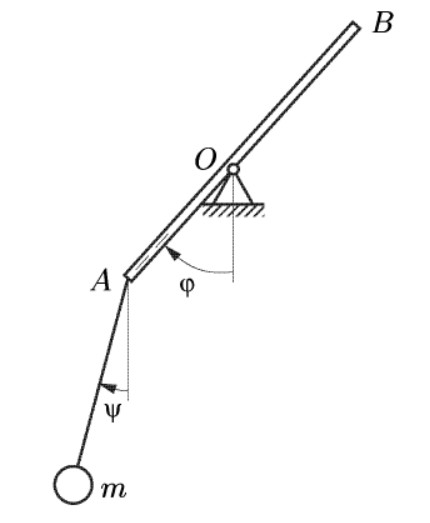
\includegraphics[width=0.9\textwidth]{figures/15_13.png}
    \caption{К задаче 15.13}
\end{minipage}
\end{figure}


\subsubsection*{15.5}


Перейдём в СО, вращающуюся вместе с телом. В таком случае в уравнениях <<возникнут>>  силы инерции. Ввиду того что $\vc{\omega} \bot \vc{r}$ запишем 
\begin{equation*}
    \vc{F}_{\text{и}} = m \vc{\omega} \times \vc{\omega} \times (\vc{r} + \vc{l}) + m \vc{\omega} \times \vc{\omega} \times \left( \vc{r} - \vc{l}\right) =
    2 m\vc{\omega} \times \vc{\omega} \times \vc{r} = 2m\omega^2 r.
\end{equation*}
Тогда добавка к потенциалу системы будет
\begin{equation*}
    \Pi_{\text{и}} = - \omega^2 r^2 m.
\end{equation*}
Силы между гантелями и стержнем аналогичны потенциалу
\begin{equation*}
    \Pi_{\text{g}} = 
    - \frac{\alpha m}{\rho} \times 2, \hspace{0.5cm} 
    \rho = \sqrt{r^2 + l^2},
\end{equation*}
где $r$ -- расстояние от центра до стержня. 
 
Запишем теперь потенциал системы
\begin{equation*}
    \Pi =  - \frac{2\alpha m}{\rho} - \omega^2 r^2 m.
\end{equation*}
Найдём стационарные точки потенциала
\begin{equation*}
    \frac{\partial \Pi}{\partial r} = \frac{2\alpha m r}{(r^2+l^2)^{3/2}} 
    -
    2 \omega^2 r m = 2mr \left(
        \frac{\alpha}{(r^2+l^2)^{3/2}} - \omega^2
    \right) = 0
    \hspace{0.5cm} \Rightarrow \hspace{0.5cm} 
    \left\{\begin{aligned}
        r_1^* &= \sqrt{\left({\alpha}/{\omega^2} \right)^{2/3} - l^2}
        , &\omega^2 l^3 < \alpha. \\
        r_2^* &= 0.
    \end{aligned}\right.
\end{equation*}
И определим локальные экстремумы потенциала
\begin{equation*}
    \frac{\partial^2 \Pi}{\partial r^2} (r) =
    2 m
    \left(
    \frac{\alpha}{(r^2+l^2)^{3/2}} -
    \frac{\alpha r^2}{(r^2+l^2)^{5/2}} - \omega^2
    \right).
    .
\end{equation*}
При $r = r^*_2$ верно, что
\begin{equation*}
    \frac{\partial^2 \Pi}{\partial r^2} (0) = 
    \frac{2\alpha}{l^3} - 2 \omega^2,
    \hspace{0.5cm} \Rightarrow \hspace{0.5cm} 
    \left\{\begin{aligned}
        r^* = 0 &\text{\ -- устойчиво при } 
        &\omega^2 l^3 < \alpha, \\
        r^* = 0 &\text{\ -- неустойчиво при } 
        &\omega^2 l^3 > \alpha.
    \end{aligned}\right.    
\end{equation*}
Чуть сложнее для $r = r^*_1$, заметим, что случай реализуется только при $\omega^2 l^3 < \alpha$:
\begin{equation*}
    \frac{\partial^2 \Pi}{\partial r^2} (r^*_1)= 
    \underbrace{\left(\ \ldots\ \right)}_{>0}
    \left(
        \alpha^{-2/3} \omega^{4/3} l^2 - 1
    \right),
    \hspace{0.5cm} a^{-2/3} < \omega^{-4/3} l^{-2}
    \hspace{0.5cm} \Rightarrow \hspace{0.5cm} 
    \frac{\partial^2 \Pi}{\partial r^2} (r^*_1) < 0.
\end{equation*}
Таким образом $r = r^*_1$ -- неустойчивое положение равновесия.


\subsubsection*{15.9}

Параметризуем систему некоторым $\varphi$ таким, что
\begin{equation*}
    \left\{\begin{aligned}
        x &= a \sin \varphi \\
        y &= b \cos \varphi
    \end{aligned}\right.
    \hspace{0.5cm} \Rightarrow \hspace{0.5cm} 
    \frac{x^2}{a^2} + \frac{y^2}{b^2}  = 1.
\end{equation*}
Аналогично предыдущим задачам считаем, что движение происходит в поле потенциальных сил (инерции и гравитации):
\begin{equation*}
    \Pi_{\text{g}} = mgy  = mgb \cos \varphi,
    \hspace{0.5cm} 
    \Pi_{\text{и}} = - \frac{1}{2} m \omega^2 x^2 = - \frac{1}{2} m \omega^2 a^2 \sin^2 \varphi.
\end{equation*}
Далее полагая $m=1$, найдём стационарные точки потенциала
\begin{equation*}
    \frac{\partial \Pi}{\partial \varphi} =
    \sin \varphi \frac{1}{\omega^2 a^2} 
    \left(
        \cos \varphi + \frac{bg}{\omega^2 a^2} 
    \right) = 0,
    \hspace{0.5cm} \Rightarrow \hspace{0.5cm} \left\{\begin{aligned}
        \sin \varphi^* &= 0 \\
        \cos \varphi^* &= - \frac{bg}{\omega^2 a^2}, &bg < \omega^2 a^2 
    \end{aligned}\right.
\end{equation*}
и определим локальные экстремумы потенциала
\begin{equation*}
    \frac{\partial^2 \Pi}{\partial \varphi^2} = \omega^2 a^2  
    \left(1 - 2\cos^2 \varphi\right) - bg \cos \varphi.
\end{equation*}
Для $\sin \varphi^* = 0$ и, соответсвенно, $\cos \varphi = \pm 1$, найдём, что
\begin{equation*}
    \frac{\partial^2 \Pi}{\partial \varphi^2} (\varphi^*) = 
    - \omega^2 a^2 \mp bg,
    \hspace{0.5cm} \Rightarrow \hspace{0.5cm} 
    \left\{\begin{aligned}
        &(0, b) \text{\ \ \ \, -- неустойчиво при \ } &\omega^2 a^2 < bg, \\
        &(0, -b) \text{\ \ -- устойчиво при \ } &\omega^2 a^2 < bg, \\
        &(0, \pm b) \text{\ \ -- неустойчиво при \ } &\omega^2 a^2 > bg. \\
    \end{aligned}\right.
\end{equation*}
Для $\cos \varphi^* = - bg / \omega^2 a^2$, и соответсвующего $\sin \varphi^*$ найдём, что при $\omega^2 a^2 > gb$
\begin{equation*}
    \frac{\partial^2 \Pi}{\partial \varphi^2} (\varphi^*) = 
    \left(
    1 + \frac{bg}{\omega^2 a^2} 
    \right) \left(
        \omega^2 a^2 - bg
    \right),
    \hspace{0.5cm} \Rightarrow \hspace{0.5cm} 
    \left(\pm a\sqrt{1 - \frac{g^2b^2}{\omega^4a^4}}, - b\frac{gb}{\omega^2a^2} \right)
    \text{\ \ -- устойчивые.}
\end{equation*}






\subsubsection*{15.13}


Запишем потенциал поля гравитационных сил:
\begin{equation*}
    \Pi =
     \frac{1}{2} \frac{l_2}{l_1+l_2} M g l_2 -
     \frac{1}{2} \frac{l_1}{l_1+l_2} M g l_1 -
     \left(
        l_1 \cos \varphi + l \cos \psi
     \right) m g.
\end{equation*}
Заметим, что в $\Pi$ независимо входит $\cos \psi$, в силу $\Pi \to \min$ имеет, что $\cos \psi = 1, \ \psi = 0$. Так как связь односторонняя, то невозможно значение $\psi = \pi$. Далее будем решать одномерую задачу. 

Найдём стационарные точки потенциала
\begin{equation*}
    \frac{\partial \Pi}{\partial \varphi} 
    = 
    \frac{1}{2} \frac{M g }{l_1 + l_2} (\sin \varphi) 
    \left(-l_2^2 + l_1^2 + 2l_1 (l_1 + l_2) \frac{m}{M} \right),
    \hspace{0.5cm} \Rightarrow \hspace{0.5cm} 
    \left\{\begin{aligned}
        \sin \varphi^* &= 0 \\
        2 m l_1 &= M(l_2 - l_1)         &\forall \varphi \text{ \ система равновесна}.
    \end{aligned}\right.
\end{equation*}
И опредлеим локальные экстремумы
\begin{equation*}
    \frac{\partial^2 \Pi}{\partial \varphi^2} =
    \underbrace{(\ \ldots \ )}_{> 0 } (\cos \varphi)
    \left(M(l_1 - l_2) + 2l_1 m\right),
    \hspace{0.5cm} \Rightarrow \hspace{0.5cm} 
    \left\{\begin{aligned}
        \varphi &= 0 \text{ -- устойчиво при } &2ml_1 > M(l_2-l_1) \\
        \varphi &= \pi \text{ -- устойчиво при } &2ml_1 < M(l_2-l_1) \\
    \end{aligned}\right.
\end{equation*}
и соотвествующие положения равновесия неустойчивы при обратных знаках в неравенствах.
\subsubsection*{15.23}


% \begin{wrapfigure}{r}{0.3\textwidth}
%   \begin{center}
%         \vspace{-20 mm}
%         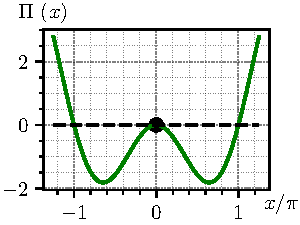
\includegraphics{figures/15_23.pdf}
%   \end{center}
%     \caption{График $\Pi(x) = -x\sin x$}
% \end{wrapfigure}

\begin{figure}
    \centering
    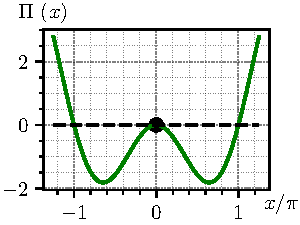
\includegraphics{figures/15_23.pdf}
    \caption{График $\Pi(x) = -x\sin x$}
\end{figure}


Начнём с того, что условие не корректно. 
Действительно, давайте посмотрим на близкие к $0$ положения равновесия системы с потенциалом $\Pi(x) = -x \sin x$. В точке $x=0$ существует неустойчивое положение равновесия, однако посмотрим на развитие системы из точки $\{-\pi-\delta, 0\}$, увидим, что на фазовой плоскости существует замкнутая орбита (сплюснутая в середине), содержащая $x=0$. Поэтому докажем, что при наличие устойчивого равновесия, существует замкнутая кривая на фазовой плоскости. 

Также хотелось бы что-то сказать при наличие замкнутой траектории о положении равновесия. Можно показать, что при отсутствие других положений равновесия в этой области положение равновесия будет устойчивым. Аналогично можно считать, что положение равновесия устойчиво только если для любой $U_\varepsilon$ окрестности существует замкнутая траектория вложенная в $U_\varepsilon$ и содержащая точку.

Так как сила $F = F(x)$ и $F(x)$ гладкая, то всегда можно ввести потенциал такой, что
\begin{equation*}
    -\frac{\partial \Pi(x)}{\partial x} = F(x) = \ddot{x}.
\end{equation*}
Также можно считать, что энергия системы сохраняется, то есть
\begin{equation*}
    E = \Pi(x) + \frac{1}{2} \dot{x}^2 = \const.
\end{equation*}

Пусть есть устойчивое положение равновесия $x^*$, тогда мы знаем, что
\begin{equation*}
    -\frac{\partial \Pi}{\partial x} (x^*) = 0, \hspace{0.5cm} \frac{\partial^2 \Pi}{\partial x^2} (x^*) > 0.
\end{equation*}
Тогда возьмём в в качетсве крайних точек нашей траектории $x_1 = x^* - \delta_1$ и в качетсве $x_2 = x^* + \delta_2$, где $\delta_i$ -- достаточно малая величина, чтобы $x' \notin U_\delta (x^*)$, $x' $ -- другое положение равновесия/точка перегиба потенциала. Выберем $\delta_1, \delta_2$ так, чтобы
\begin{equation*}
    \Pi(x^* - \delta_1) = \Pi(x^* + \delta_2).
\end{equation*}
Тогда поместив с 0 скоростью точку $x_1$ получим замкнутую орбиту $[x_1, \ x_2]$.

В другую сторону, пусть есть некоторая замкнутая орбита на $[x_1, \ x_2]$. Тогда верно, что
\begin{equation*}
    T(x_1) = T(x_2) = 0, \hspace{0.5cm} 
    -\frac{\partial \Pi}{\partial x} (x_1) > 0, \hspace{0.5cm} 
    -\frac{\partial \Pi}{\partial x} (x_2) < 0.
\end{equation*}
Тогда по непрерывности $\Pi(x)$ существует $x^*$ такой, что $\partial \Pi(x^*) / \partial x = 0$, при чём, так как это единственная точка экстремума потенциала в $[x_1, \ x_2]$, то это минимум, $\partial^2 \Pi / \partial x (x^*) > 0$, Q. E. D. %done


\section{Контрольная работа II}

\subsection*{Задача №1}

Рассмторим движение твёржого тела с неподвижной точкой $O$, в частности рассмотрим случай Лагранжа. Хотелось бы найти первые инегралы и какое-нибудь хорошее дифференциальное уравнение для системы, при условии что $(\vc{K}_O)_z = 0$ и $\omega_\xi = 0$.

Запишем кинематические и динамические уравнения Эйлера: 
\begin{equation*}
    \left\{\begin{aligned}
        p &= \dot{\psi} \sin \theta \sin \varphi + \dot{\theta} \cos \varphi,\\
        q &= \dot{\psi} \sin \theta \cos \varphi - \dot{\theta} \sin \varphi,\\
        r &= \dot{\psi} \cos \theta + \dot{\varphi}.
    \end{aligned}\right.,
    \hspace{0.6cm} 
    \left\{\begin{aligned}
        I_1 \dot{p} + (I_3-I_2) q r &= M_{\xi} \\
        I_2 \dot{q} + (I_1-I_3) p r &= M_{\eta} \\
        I_3 \dot{r} + (I_2-I_1) p q &= M_{\zeta} \\
    \end{aligned}\right.,   
    \hspace{0.6cm} 
    \hat{J}_O = \dmat{3}{I_1}{I_1}{I_3}, \hspace{0.6cm} 
    \vc{\omega} = \begin{pmatrix}
        p \\ q \\ r
    \end{pmatrix}.
\end{equation*}
При чём в случае Лагранжа сразу находим первый интеграл системы:
\begin{equation}
    \vc{M}_O = \vv{OP} \times (m \vc{g}), 
    \hspace{0.5cm} \Rightarrow \hspace{0.5cm} 
    c \dot{r} = M_{\xi} = 0,
    \hspace{0.5cm} \Rightarrow \hspace{0.5cm} 
    \dot{\psi} \cos \theta + \dot{\varphi} = r =\const.
\end{equation}
По условию $(\vc{K}_O)_z = 0$ и $\omega_\xi = 0$. В таком случае энергия системы 
\begin{equation*}
    T + \Pi = \frac{1}{2} A (p^2 + q^2) + mgl \cos \theta = \const = \frac{h}{2}.
\end{equation*}
Подставляя значения из кинематических уравнений, получаем
\begin{equation}
    A \left(
        \dot{\psi}^2 \sin^2 \theta + \dot{\theta}^2
    \right) + 2mgl \cos \theta = h = \const.
\end{equation}
Так как $(\vc{K}_0)_z = \const = 0$, то 
\begin{equation*}
    C r \cos \theta + A \dot{\psi} \sin^2 \theta = (\vc{K}_0)_z = 0,
    \hspace{0.5cm} \Rightarrow \hspace{0.5cm} 
    A \dot{\psi} \sin^2 \theta = 0.
\end{equation*}
Из последних двух выражений находим, что
\begin{equation}
    A \dot{\theta}^2 + 2 mgl \cos \theta = h,
    \hspace{0.5cm} \Rightarrow \hspace{0.5cm} 
    \boxed{
        \ddot{\theta} = \frac{mgl}{A} \sin \theta
    },
\end{equation}
что и является искомым дифференциальным уравнением второго порядка, относительно угла нутации.




\begin{figure}[h]
    \centering
    \begin{minipage}[t]{0.45\textwidth}
        \begin{center}
            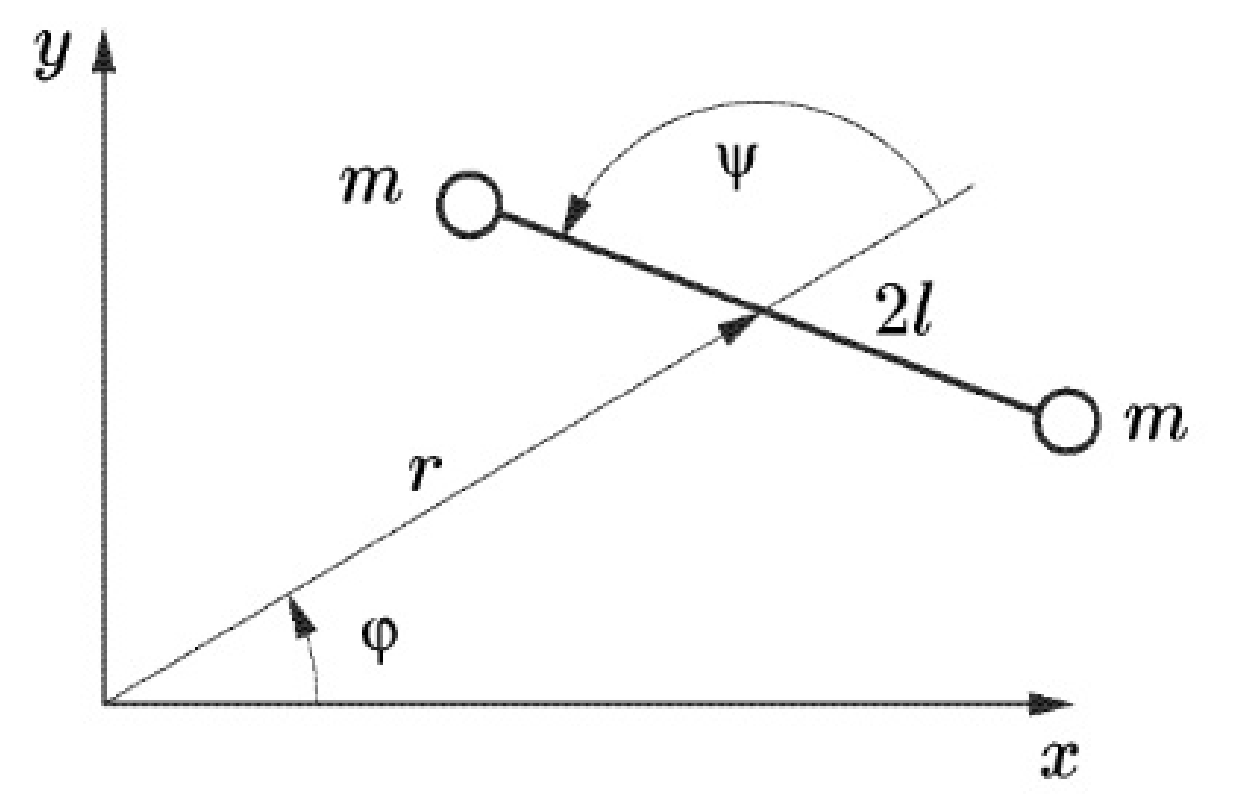
\includegraphics[width=0.65\textwidth]{figures/cw2.png}
        \end{center}
        \caption{К задаче №2}
        \label{cw_t2_2}
    \end{minipage}
    \hspace{0.5cm} 
    \begin{minipage}[t]{0.45\textwidth}
        \begin{center}
            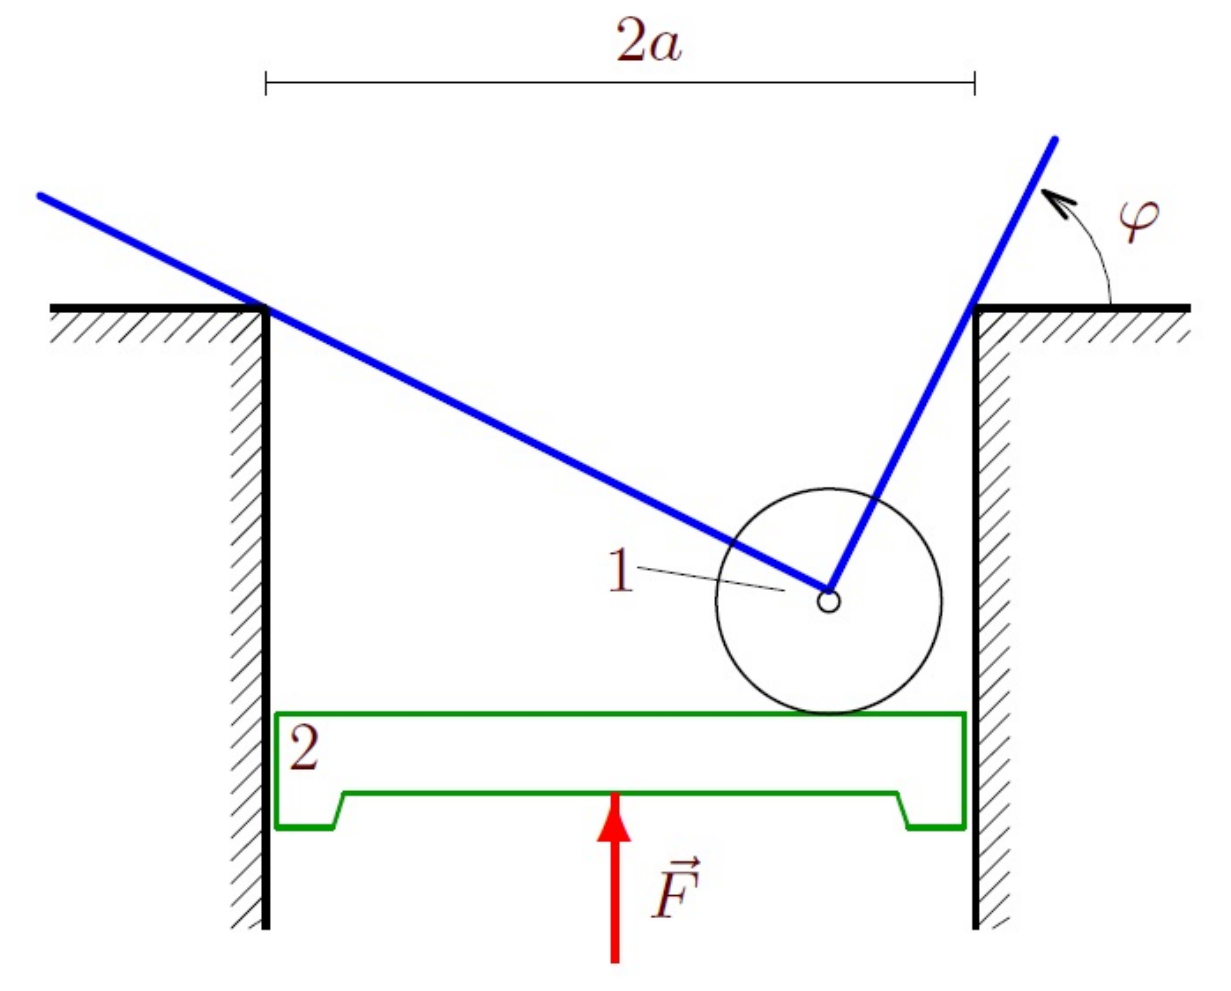
\includegraphics[width=0.65\textwidth]{figures/cw3.png}
        \end{center}
        \caption{К задаче №3}
        \label{cw_t2_3}
    \end{minipage}
\end{figure}


\subsection*{Задача №2}

Для системы, представленной на рис. \ref{cw_t2_2} найдём лагранжиан. Потенциальная энергия системы (считая, что в $(0,0)$ находится тело массы $M \gg m$),
\begin{equation*}
    \Pi = - \frac{2GMm}{r} \overset{\mathrm{def} \varkappa}{=} - \varkappa \frac{m}{r} .
\end{equation*}
Положение массивных тел, из геометрии системы, можем записать, как
\begin{equation*}
    r_{1,\,2} = r \begin{pmatrix}
        \cos \varphi \\
        \sin \varphi 
    \end{pmatrix} 
    \pm l \begin{pmatrix}
        - \cos (\varphi + \psi) \\
        \phantom{-} \sin (\varphi + \psi)
    \end{pmatrix}.
\end{equation*}
Кинетиечская энергия системы теперь может быть записана как
\begin{equation*}
    T = \frac{m}{2} \left(
        \dot{r}^2_1 + \dot{r}^2_2
    \right),
\end{equation*}
где
\begin{equation}
\left\{\begin{aligned}
    \dot{r}_1 = \dot{r} \begin{pmatrix}
        \cos \varphi \\
        \sin \varphi  
    \end{pmatrix} + r \begin{pmatrix}
        - \sin \varphi \\
        \phantom{-}  \cos \varphi
    \end{pmatrix}
    \dot{\varphi} + 
    l \begin{pmatrix}
        \sin (\varphi + \psi) \\
        \cos (\varphi + \psi) \\
    \end{pmatrix} (\dot{\varphi} + \dot{\psi}), \\
    \dot{r}_2 = \dot{r} \begin{pmatrix}
        \cos \varphi \\
        \sin \varphi  
    \end{pmatrix} + r \begin{pmatrix}
        - \sin \varphi \\
        \phantom{-}  \cos \varphi
    \end{pmatrix}
    \dot{\varphi} - 
    l \begin{pmatrix}
        \sin (\varphi + \psi) \\
        \cos (\varphi + \psi) \\
    \end{pmatrix} (\dot{\varphi} + \dot{\psi}), \\
\end{aligned}\right.
\end{equation}
что позволяет, наконец, записать лагранжиан системы
\begin{equation}
    L = T - \Pi,
    \hspace{0.5cm} \Rightarrow \hspace{0.5cm} 
    L / m =  \dot{r}^2 + r^2 \dot{\varphi}^2 + l^2 \left(\dot{\varphi}+ \dot{\psi}\right)^2 + \frac{\varkappa}{r} .
\end{equation}
Так как на систему действуют только радиальные силы, то
\begin{equation}
    \frac{d \vc{K}_O}{d t} = \vc{M}_O = 0, 
    \hspace{0.5cm} \Rightarrow \hspace{0.5cm} 
    \vc{r}_1 \times \dot{\vc{r}}_1 + \vc{r}_2 \times \dot{\vc{r}}_2 = \const.
\end{equation}
Также сохраняется энергия системы,
\begin{equation}
    T + \Pi = \const, 
    \hspace{0.5cm} \Rightarrow \hspace{0.5cm} 
     \dot{r}^2 + r^2 \dot{\varphi}^2 + l^2 \left(\dot{\varphi}+ \dot{\psi}\right)^2 + \frac{\varkappa}{r} = \const.
\end{equation}

\subsection*{Задача №3}

Аналогично предыдущей задачи, найдём уравнения движения системы (рис. \ref{cw3}) в форме Лагранжа. Выберем в качестве начала координат правый верхний угол системы,выбрав оси, как показано на рисунке. По всей видимости будем считать в угла стержни <<прикрепленными>> к опорам так, чтобы не было отрыва -- иначе задача не имеет смысла. 

\begin{figure}[h]
    \centering
    \incfig{cw3}
    \caption{К задаче №3}
    \label{cw3}
\end{figure}

Так как на платформу действует постоянная сила $\vv{F}$, потенциальная энергия системы
\begin{equation*}
    \vc{\tilde g} = \vc{g} + \frac{\vv{F}}{m_1+m_2}  = \vc{g} + 3 \vc{g} = 4 \vc{g},
    \hspace{0.5cm} 
    \Pi = - (m_1 + m_2) \vc{\tilde g} y_1.
\end{equation*}
Координаты диска и платформы, соотвественно
\begin{equation*}
    \vc{r}_{\text{д}} = \vc{r}_1 = \begin{pmatrix}
        x_1 \\ y_1
    \end{pmatrix} = 
    \begin{pmatrix}
        l_2 \cos \varphi \\
        l_2 \sin \varphi.
    \end{pmatrix},
    \hspace{0.5cm} 
    \vc{r}_{\text{п}} = \vc{r}_1 = \begin{pmatrix}
        0 \\
        l_2 \sin \varphi + R
    \end{pmatrix}.
\end{equation*}
Из геометрии системы, можем понять, что
\begin{equation*}
    l_2 / 2a = \cos \varphi, \hspace{0.5cm} \Rightarrow \hspace{0.5cm} 
    \left\{\begin{aligned}
        x_1 = 2 a \cos^2 \varphi \\
        y_1 = a \sin (2\varphi).
    \end{aligned}\right.
\end{equation*}
Дифференцируя по времени, найдём скорость диска:
\begin{equation*}
    \dot{\vc{r}}_1 = 2 a \dot{\varphi} \begin{pmatrix}
        - \sin 2 \varphi \\
        \phantom{-} \cos 2 \varphi
    \end{pmatrix}, \hspace{0.25cm} 
    \omega R = \dot{x}_1
    \hspace{0.5cm} \Rightarrow \hspace{0.5cm} 
    \omega^2 = \frac{1}{R^2} 4 a^2 \dot{\varphi}^2 \sin^2 2 \varphi.
\end{equation*}
Кинетическая энергия диска, как сумма поступательной и вращательной
\begin{equation*}
    T_1 = \frac{1}{2} \left(\frac{m_1 R^2}{2} \right) \frac{1}{R^2} 4 a^2 \dot{\varphi}^2 \sin^2 2 \varphi + 2 a^2 \dot{\varphi}^2 m_1.
\end{equation*}
Для платформу кинетическая энергия, соотвественно
\begin{equation*}
    T_2 = \frac{m_2}{2} \dot{y}_1^2.
\end{equation*}
К огромному счастью трудящихся полная кинетическая энергия системы оказывается равна
\begin{equation*}
    T = T_1 + T_2 = 6 m_2 a^2 \dot{\varphi}^2.
\end{equation*}
Лагранжиан системы
\begin{equation}
    L = T - \Pi = 6m_2 a\left(
        a \dot{\varphi}^2 + 2 g \sin 2 \varphi
    \right).
\end{equation}
Запишем уравнение Лагранжа второго рода:
\begin{equation}
    \frac{d}{dt} \frac{\partial L}{\partial \dot{\varphi}} - \frac{\partial L}{\partial \varphi} = 0, \hspace{0.5cm} \Rightarrow \hspace{0.5cm} 
    \ddot{\varphi} = \frac{2g}{a} \cos (2 \varphi).
\end{equation}
Решение этого дифференциального уравнения в терминах аналитических функций не представляется возможным, однако можем посмотреть на происходящее вблизи положения равновесия:
\begin{equation*}
    \ddot{\varphi} = 0, \hspace{0.5cm} \Leftrightarrow \hspace{0.5cm} 
    \varphi = \pi / 4.
\end{equation*}
В таком случа рассмотрим $\alpha \colon 2 \varphi = \pi/2 + \alpha$,
\begin{equation}
\boxed{
     \ddot{\alpha} = - \omega^2 \sin \alpha,   
}
    \hspace{0.5cm} \omega^2 = \frac{4g}{a}.
\end{equation}
И, при малых $\alpha$, получили гармонический осциллятор:
\begin{equation*}
    \alpha = C_1 \sin \omega t + C_2 \cos \omega t.
\end{equation*}
Из начальных условий (при $t=0$ $\varphi = \varphi_0$), находим, что
\begin{equation*}
    \varphi(t) = \frac{\pi}{4} + \left(\varphi_0 - \frac{\pi}{4} \right) \cos \omega t,
    \hspace{0.5cm} 
    \dot{\varphi} = \left(\frac{\pi}{4} - \varphi_0\right) \omega \sin \omega t.
\end{equation*}
Если нас интересует угловая скорость $\dot{\varphi}$ в момент, когла $\varphi = \varphi_1$, то
\begin{equation}
    \dot{\varphi}(t_1) = \pm 2 \sqrt{\frac{g}{a} } \cdot \sqrt{
        \left(\varphi_1 + \varphi_0 - \frac{\pi}{2}\right) (\varphi_1 - \varphi_0)
    },
    \hspace{0.5cm} 
    0 < \varphi_0 - \pi/4 < \varphi_1 - \pi/4 \ll 1.
\end{equation}


